\documentclass[a4paper, openany, 12pt]{book}
\usepackage[usenames,dvipsnames,svgnames,table]{xcolor}
\usepackage{pdfpages}
\usepackage{etoolbox}
\usepackage{multirow}
\usepackage{vmargin}
\usepackage{rotating}
\usepackage{subfigure}
\usepackage[utf8]{inputenc}
\usepackage{biblatex}
\usepackage[backend=biber]{biblatex}
\usepackage{graphicx}
\usepackage{subfigure}
\usepackage{appendix}
\usepackage{float}
\usepackage{multicol}
\usepackage{tocloft}
\usepackage[spanish]{babel}
\usepackage[utf8]{inputenc}
\usepackage{makeidx}
\usepackage{lscape}
\usepackage{color}
\usepackage{hhline}
\usepackage{longtable}
\usepackage{wrapfig} %preámbulo
\floatstyle{}
\usepackage{titlesec}
\usepackage[ backend=biber, style=numeric, citestyle=ieee,sorting=none]{biblatex}

\addbibresource{references.bib}
\setcounter{secnumdepth}{4}
\setcounter{tocdepth}{4}
%-estilo de pagina---------------
\usepackage{fancyhdr}
\pagestyle{fancy}
\renewcommand{\chaptermark}[1]{\markboth{#1}{}}
\renewcommand{\sectionmark}[1]{\markright{\thesection\ #1}}
\renewcommand{\headrulewidth}{0.4pt}
\fancyhead{}
\fancyfoot{}
\fancyhead[LO]{\emph\leftmark}
\fancyhead[RE]{\emph\rightmark}
\fancyfoot[C]{\thepage}
%=================---definir estilo y color de los nombres de capitulos y secciones
\definecolor{AzulClaro}{rgb}{0.2,0.5,0.7}
\definecolor{Veeerde}{rgb}{0.0, 0.42, 0.24}
%\newfontfamily{\coral}{TeX Gyre Chorus}
%\newfontfamily{\coral}{roman}
%=======--definir cuadro de texto
\usepackage{tcolorbox}
%\tcbuselibrary{listingsutf8} % o listings o minted
\tcbuselibrary{listings}
%=============================
\titleformat{\chapter}[frame]
{\LARGE\coral\bfseries\color{AzulClaro}}{\filright\chaptertitlename\ \thechapter}{20pt}{\Huge}
%\titleformat*{\section}{\Large\bfseries\sffamily\color{Veeerde}}
\titleformat*{\section}{\Large\bfseries\color{Veeerde}}


%------INICIO DOCUMENTO-------------------------
\begin{document}
\renewcommand{\tablename}{Tabla}
\thispagestyle{empty}
%--------------------------
%---portada 1-----------------------------------
\renewcommand{\tablename}{Tabla}
\thispagestyle{empty}
\begin{center}

\includegraphics[width=0.5 \textwidth]{imagenes/logoUTB_BW.jpg} \\
\vspace{1.0cm}
{\large \textbf{Facultad de Ciencias Básicas} \\
\vspace{0.15cm}
{\large \textbf{Maestría en Estadística Aplicada}}

\vspace{2.5cm}
{\Large\color{AzulClaro} \textbf{Reconocimiento de placas vehiculares usando redes neuronales convolucionales}
}\\
\vspace{2.5cm}

Autor \\
\vspace{0.70cm}
{\large \textbf{Didier Eloy Arroyo Pérez}
}\\


\vspace{4.0cm}
Cartagena de Indias\\
\vspace{0.25cm}
2020
}
\end{center}
\newpage
%-----portada 2-----------------
\begin{center}

\includegraphics[width=0.5 \textwidth]{imagenes/logoUTB_BW.jpg} \\
\vspace{1.0cm}
{\large \textbf{Facultad de Ciencias Básicas} \\
\vspace{0.15cm}
{\large \textbf{Maestría en Estadística Aplicada}}

\vspace{2.5cm}
{\Large\color{AzulClaro} \textbf{Reconocimiento de placas vehiculares usando redes neuronales convolucionales}
}\\
\vspace{1.5cm}

Autor \\
\vspace{0.25cm}
{\large \textbf{Didier Eloy Arroyo Pérez}
}\\
\vspace{2.0cm}
Director: Alberto Patiño Vanegas, Ph.D\\
\vspace{0.25cm}
Co-director: Alberto Patiño Saucedo, Ph.D (C)\\

\vspace{3.0cm}
Cartagena de Indias\\
\vspace{0.25cm}
2020
}
\end{center}
\newpage
\thispagestyle{empty}
%---dedicartoria---------------------
\newpage
\thispagestyle{empty}
\chapter*{Dedicatoria}
\addcontentsline{toc}{chapter}{Dedicatoria}
\markboth{Dedicatoria}{Dedicatoria}
\pagenumbering{Roman}
\setcounter{page}{1}

\begin{center}
    \vspace*{\fill}
   \noindent
	\textbf{Para mi esposa, Jessica y mis hijos, Guadalupe y Gael}.\\
   \textit{Con mucho amor y esfuerzo para su bienestar y orgullo.} 
   \vspace*{\fill}
\end{center}
   
\chapter*{Agradecimientos}
\addcontentsline{toc}{chapter}{Agradecimientos}
\markboth{Agradecimientos}{Agradecimientos}
\pagenumbering{Roman}
\setcounter{page}{2}

  \Item A Dios que siempre me ha dado fortaleza para seguir adelante.\newline

  \Item A la Universidad Tecnológica de Bolívar por abrirme sus puertas y así mejorar mi nivel profesional.\newline
  
  \Item A mi director, Alberto Patiño Vanegas, por su constante apoyo y recomendaciones.\newline
  
  \Item A mi codirector de tesis, Alberto Patiño Saucedo, por brindarme su apoyo, tiempo y guía.\newline
  
  \Item A mis colegas de la Maestría en Estadística Aplicada por acompañarme en esta etapa de formación.\newline
  
  \Item A mis padres María Nevid Pérez Herrera y Eloy Alfredo Arroyo Márquez y mis hermanas por todo el cariño, amor y apoyo que me han brindado toda mi vida.\newline
  
  \Item A mi esposa e hijos por su apoyo incondicional en toda esta etapa.\newline
  
  \Item A todas aquellas personas que de alguna manera me acompañaron en esta ruta de nuevo conocimiento y formación académica.\newline
  
%----resumen------------------------------
\chapter*{Resumen}
\addcontentsline{toc}{chapter}{Resumen}
\markboth{Resumen}{Resumen}
\pagenumbering{Roman}
\setcounter{page}{3}
 En este trabajo se diseñó y elaboró un sistema experto de visión artificial para el reconocimiento automático de placas de automóviles en Colombia. El sistema usa una imagen capturada con una cámara convencional en el rango visible del espectro electromagnético y técnicas de aprendizaje profundo. 
 Para el entrenamiento, nosotros hemos construido inicialmente una base de datos con imágenes de caracteres segmentados de placas colombianas más imágenes de caracteres depurados de la base de datos pública Chars74k. Esta base de datos se usó para entrenar una Red Neuronal Convolucional creada desde cero, lográndose un porcentaje de clasificación correcta por caracter del 99,49\%; pero al momento de reconocer toda la placa (los seis caracteres), el rendimiento disminuye al 84\% en el conjunto de prueba. Teniendo en cuenta que, la aplicación de estos sistemas exige un sistema experto de reconocimiento de placas, se decidió construir otra base de datos con las coordenadas de caracteres de placas colombianas obtenidas usando Cuadros Delimitadores (Bonding Boxing). Con esta segunda base de datos, se usó un modelo pre-entrenado de TensorFlow, basado en una Red Neuronal Convolucional mucho mas Rápida con propuesta de Regiones (Faster R-CNN). A pesar de entrenarse con una base de datos no equilibrada y con poca variabilidad se logró un mejor rendimiento que usando la red neuronal convolucional construida desde cero; lo que permite concluir que éste tipo de red promete mejores resultados si se usa una base de datos más equilibrada y con mucha variabilidad. 
 
\newpage
%-----abstract-------------------------
\chapter*{Abstract}
\addcontentsline{toc}{chapter}{Abstract}
\markboth{Resumen}{Abstract}
\pagenumbering{Roman}
\setcounter{page}{3}
In this work, an expert artificial vision system for the automatic recognition of car license plates in Colombia was designed and elaborated. The system uses an image captured with a conventional camera in the visible range of the electromagnetic spectrum and deep learning techniques.
 For training, we have initially built a database with images of segmented characters from Colombian plates plus images of depurate characters from the public Chars74k database. This database was used to train a Convolutional Neural Network created from scratch, achieving a percentage of correct classification per character of 99.49\%. But, at the moment of reconizing whole plate (all six characters), the performance drops to 84\% in the test set.
Taking into account that the application of these systems requires an expert plate recognition system, another database was decided to build with the coordinates of characters of Colombian plates obtained using Bounding Boxes. With this second database, a pre-trained TensorFlow model was used, based on a much Faster Convolutional Neural Network with proposed Regions (Faster R-CNN). Despite training with an unbalanced database and with little variability, better performance was achieved than using the convolutional neural network built from scratch; which allows us to conclude that this type of network promises better results if a more balanced database with a lot of variability is used.

\newpage

%------tabla de contenido----------------
\thispagestyle{empty}
\tableofcontents
%----listya de figuras
\clearpage
\addcontentsline{toc}{chapter}{Lista de Figuras}
\listoffigures
%----lista de tablas
\clearpage
\addcontentsline{toc}{chapter}{Lista de Tablas}
\listoftables
%----------------------------
\chapter*{Introducción}
\pagenumbering{arabic}
El reconocimiento automático de matrículas (del inglés - \textit{Automatic number plate recognition o ANPR}) es un método de vigilancia en masa que utiliza reconocimiento óptico de caracteres en imágenes para leer las matrículas de los vehículos, Llano et \textit{al} \cite{llano2010sistema}. Esta herramienta es utilizada en muchas tareas, por ejemplo: son utilizadas por la policía para la identificación de vehículos robados o que han cometido alguna infracción; como método de recaudación electrónica de peaje en las autopistas de pago; y, para la vigilancia del tráfico o controlar al acceso a lugares privados, entre otros. El ANPR se puede configurar para almacenar las imágenes, el texto de la matrícula, inclusive es posible almacenar una fotografía del conductor, Llano et \textit{al} \cite{llano2010sistema}. Estos sistemas hacen uso de una alta tecnología en países desarrollados, que hasta utilizan iluminación infrarroja y flashes para hacer posible que la cámara pueda tomar fotografías en cualquier momento del día y a larga distancia. Sin embargo, para países menos desarrollados, la detección y reconocimiento de placas es un reto, ya que no todas las imágenes capturadas con una cámara serán de buena calidad por las condiciones de iluminación, deterioro de las placas y condiciones ambientales. Además, la tecnología ANPR no puede ser copiada de una región a otra, debido a la variación entre formatos de matrículas de cada país, Shivakumara et \textit{al} \cite{Shivakumara2018}.\\

Existe una cantidad significativa de sistemas de reconocimiento de placas con diferentes grados de precisión y velocidad, Du et \textit{al} \cite{Du2013}. Algunos de esos sistemas utilizan el circuito cerrado de televisión existente o radares, y otros son diseñadas específicamente para dicha tarea, Shivakumara et \textit{al} \cite{Shivakumara2018}. Dentro de los sistemas diseñados, se destacan los que usan la técnica de \textit{Deep learning} o aprendizaje profundo, donde la extracción de patrones en los datos estudiados no se realiza manualmente, sino de forma automática. Los métodos más robustos de aprendizaje profundo involucran el uso de redes neuronales convolucionales (RNC) (del inglés - \textit{Convolutional Neural Networks - CNN}). Presentadas por LeCun et \textit{al} \cite{lecun1989backpropagation} a principios de la década de los noventa, las redes convolucionales son un ejemplo de una arquitectura de red neuronal artificial especializada. Específicamente, RNC es un tipo especial de perceptrón multicapa de avance entrenado en modo supervisado utilizando un algoritmo de aprendizaje de retropropagación de descenso de gradiente que permite la extracción automatizada de características, Marin et \textit{al} \cite{marin2013introduccion}.\\ 

Las RNC han probado ser poderosas herramientas para una amplia gama de tareas de visión computarizada, tales como reconocimiento óptico de caracteres, reconocimiento de objetos genéricos, detección de rostros en tiempo real, reconocimiento de voz, reconocimiento de placas, etc, LeCun et \textit{al} \cite{Lecun2015}. RNC automáticamente aprenden abstracciones de nivel medio y de alto nivel obtenidas a partir de datos brutos. Los resultados recientes indican que las características extraídas son extremadamente efectivas en el reconocimiento y localización de objetos en imágenes naturales, Matich et \textit{al} \cite{matich2001redes}. Los inconvenientes de los sistemas de reconocimiento están centrados en la protección de la privacidad y altas tasas de error. Entretanto, los mayores desafíos de las RNC son su alto costo computacional y la demanda de grandes cantidades de muestras para su entrenamiento. Sin embargo, de la mano de los avances tecnológicos (como: grandes almacenamientos de datos y aumento de la potencia informática, sin una gestión activa directa por parte del usuario), estos sistemas han logrado ser mucho más exactos y fiables.\\

En Colombia, hay disponibles muchos sistemas de reconocimiento de placas vehiculares, la mayoría privados y basados en el reconocimiento óptico de caracteres (\textit{Optic Character Recognition - OCR}), ninguno de ellos utiliza redes neuronales convolucionales para generar modelos matemáticos en el reconocimiento de patrones, en este caso, placas vehiculares. Además, aún es posible encontrar que los registros y controles vehiculares se hacen de forma manual, lo que involucra errores constantes y poca seguridad para el usuario, sobretodo en parqueaderos ilegales. En el presente trabajo, se desarrolla y evalúa un método computacional para el reconocimiento de placas de automóviles colombianos. Esta metodología ya ha sido implementada en Colombia para prever patrones en los sistemas financieros (previsiones de precio y tasas cambiarías), sistemas ecológicos (áreas de conservación), minería, de salud e ingeniería. Así está nueva aplicación de una red neuronal convolucional ayudaría en el sistema de tránsito y transportes, ya que permitiría controlar el acceso a parqueaderos, generar tiquetes de pago automáticos, controlar hurtos, entre otras ventajas, como la disminución del costo computacional y el fácil acceso del usuario a este tipo de sistemas.
%===========================================

%----------------------
\chapter{Planteamiento del problema}
%=============================================

%-----------------------------------
\section{Definición del problema}
%----------------------------------
En Colombia, el índice de robo de carros es cada vez mayor, segun datos de la Policía Nacional Colombiana, sólo el año 2019 los carros robados fueron 10.496, un promedio de 30 diarios (datos policia nacional colombiana). Bogotá encabeza el listado de ciudades donde más roban vehículos, seguido de Medellín, Cali, Bucaramanga y Barranquilla. Según cifras de la Policía, en Bogotá, durante el año 2018, habían sido denunciados 2.500 hurtos en parqueaderos. 
Segun un estudio realizado por Norza-Céspedes et \textit{al}, unas de las formas de controlar el hurto apunta a la prevención y disuasión \cite{PolNal}. En Colombia, un gran porcentaje de controles de entrada/salida de vehiculos son manuales y no ofrecen un sistema de registro de información que ayude a persuadir el hurto de vehiculos. 
Por otro lado, los establecimientos comerciales son cada vez más concurridos y el cliente muchas veces no encuentra sitio para parquear su automovil. Esto se debe en gran manera a que muchas personas dejan sus vehiculos en los parqueaderos de los centros comerciales, pero realmente no con el fin de realizar alguna compra; o si realizan una compra, permanecen por mucho tiempo después dentro del centro. Una solución para ello, es usar sistemas que controlen el tiempo de permanencia. En Colombia, muchos de estos controles de tiempo son manuales y además no ayudan a persuadir el hurto. Otros establecimientos utilizan software comerciales de empresas extranjeras que generalmente funcionan como una "caja negra" que cuando falla, el centro debe realizar el control manualmente ocasionando retrasos y congestionamiento. Además no permite la retroalimentación para corregir los errores. 
Una solución, tanto para disuadir el hurto de vehiculos como para descongestionar los parqueaderos, es implementar sistemas de inteligentes de visión artificial que aprovechen toda la tecnología actual y el avance de las ciencias de la computación. 
El problema de reconocimiento de placas de automoviles en Colombia plantea varios retos:
\begin{enumerate}
    \item Reconocer las placas de automoviles aun estando deterioradas, tal como lo muestra la figura \ref{fig:deteriorada}; 
     %--------------------
  \begin{figure}[H]
\begin{center}
   {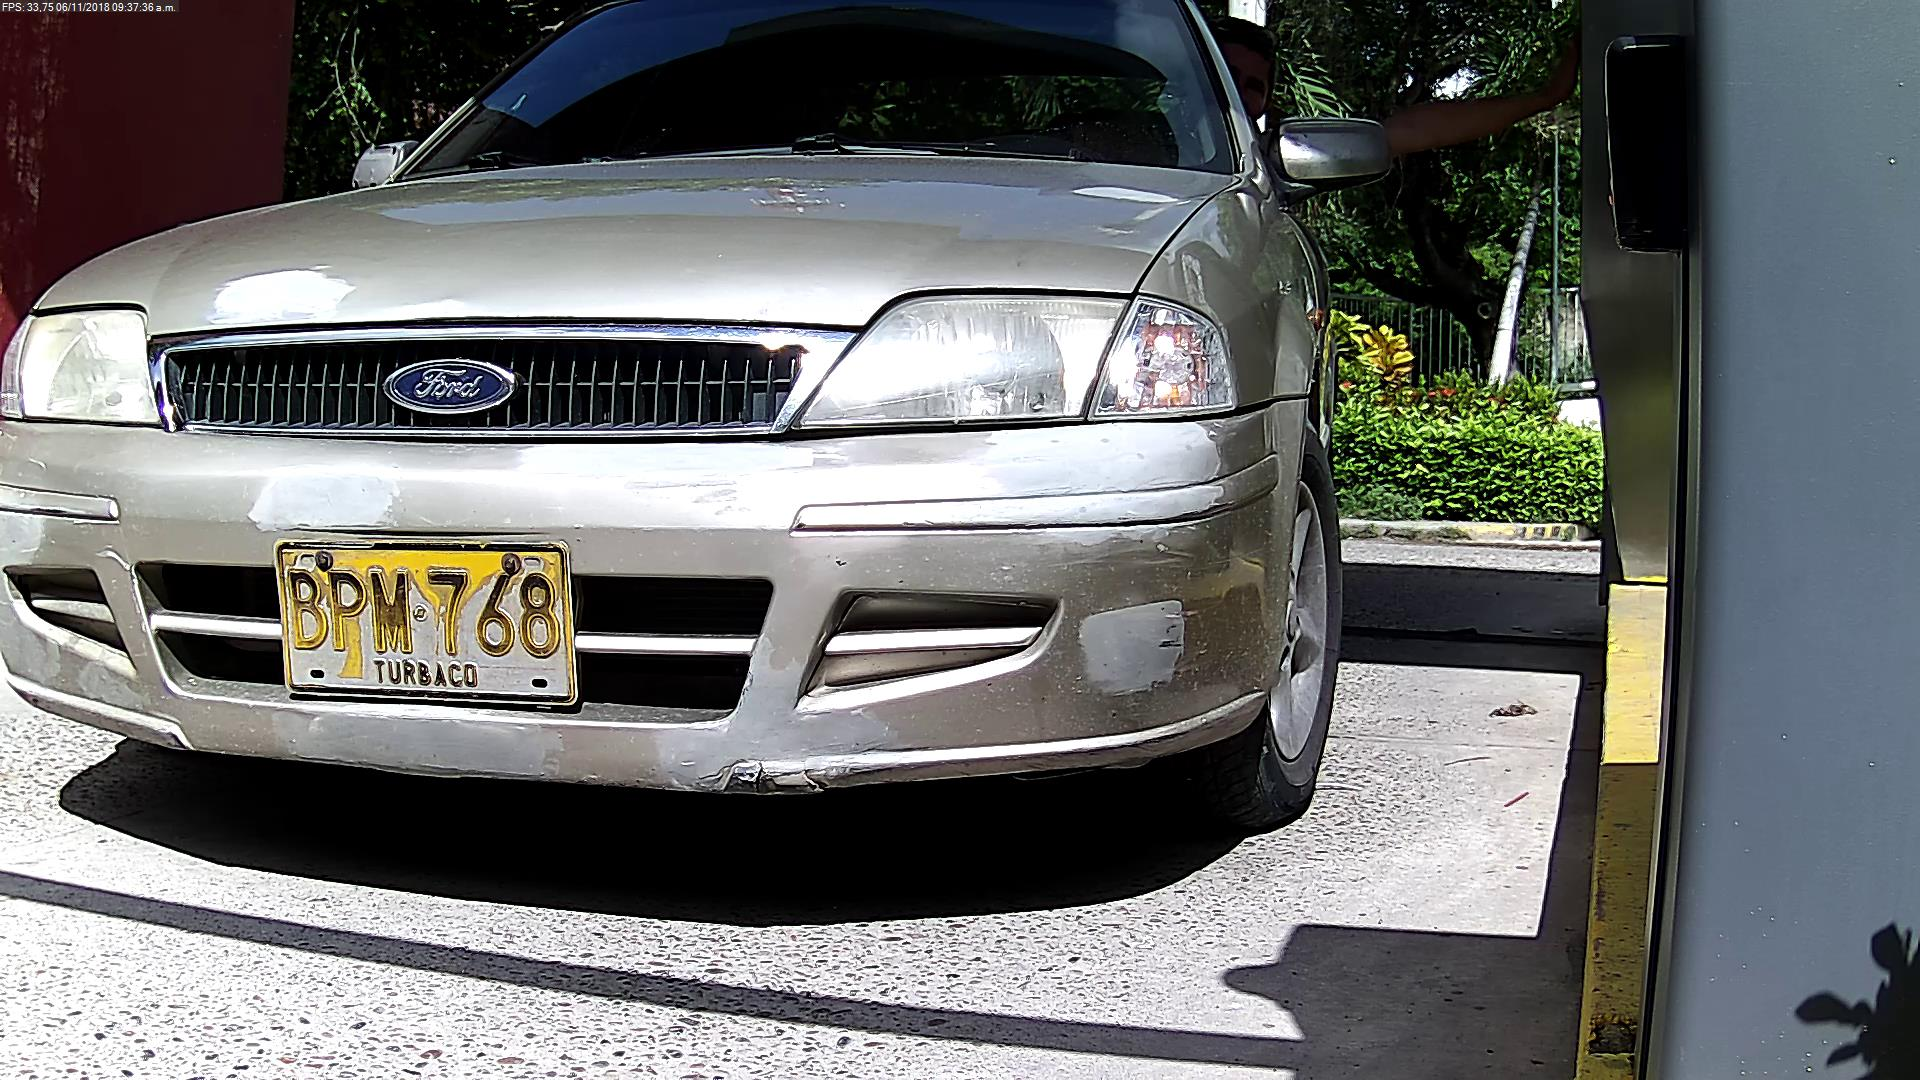
\includegraphics[width=0.8 \linewidth]{imagenes/Deterioradas/deteri.jpg}}
    \caption{Placa de automóvil con deterioro}
    \label{fig:deteriorada} 
\end{center}
\end{figure}
  %----------------------
\item Reconocer las placas de automoviles bajo condiciones ambientales adversas (iluminación, lluvia, etc), tal como lo muestra la figura \ref{fig:adversas}; 
    %--------------------
    \begin{figure}[H]
\begin{center}
   {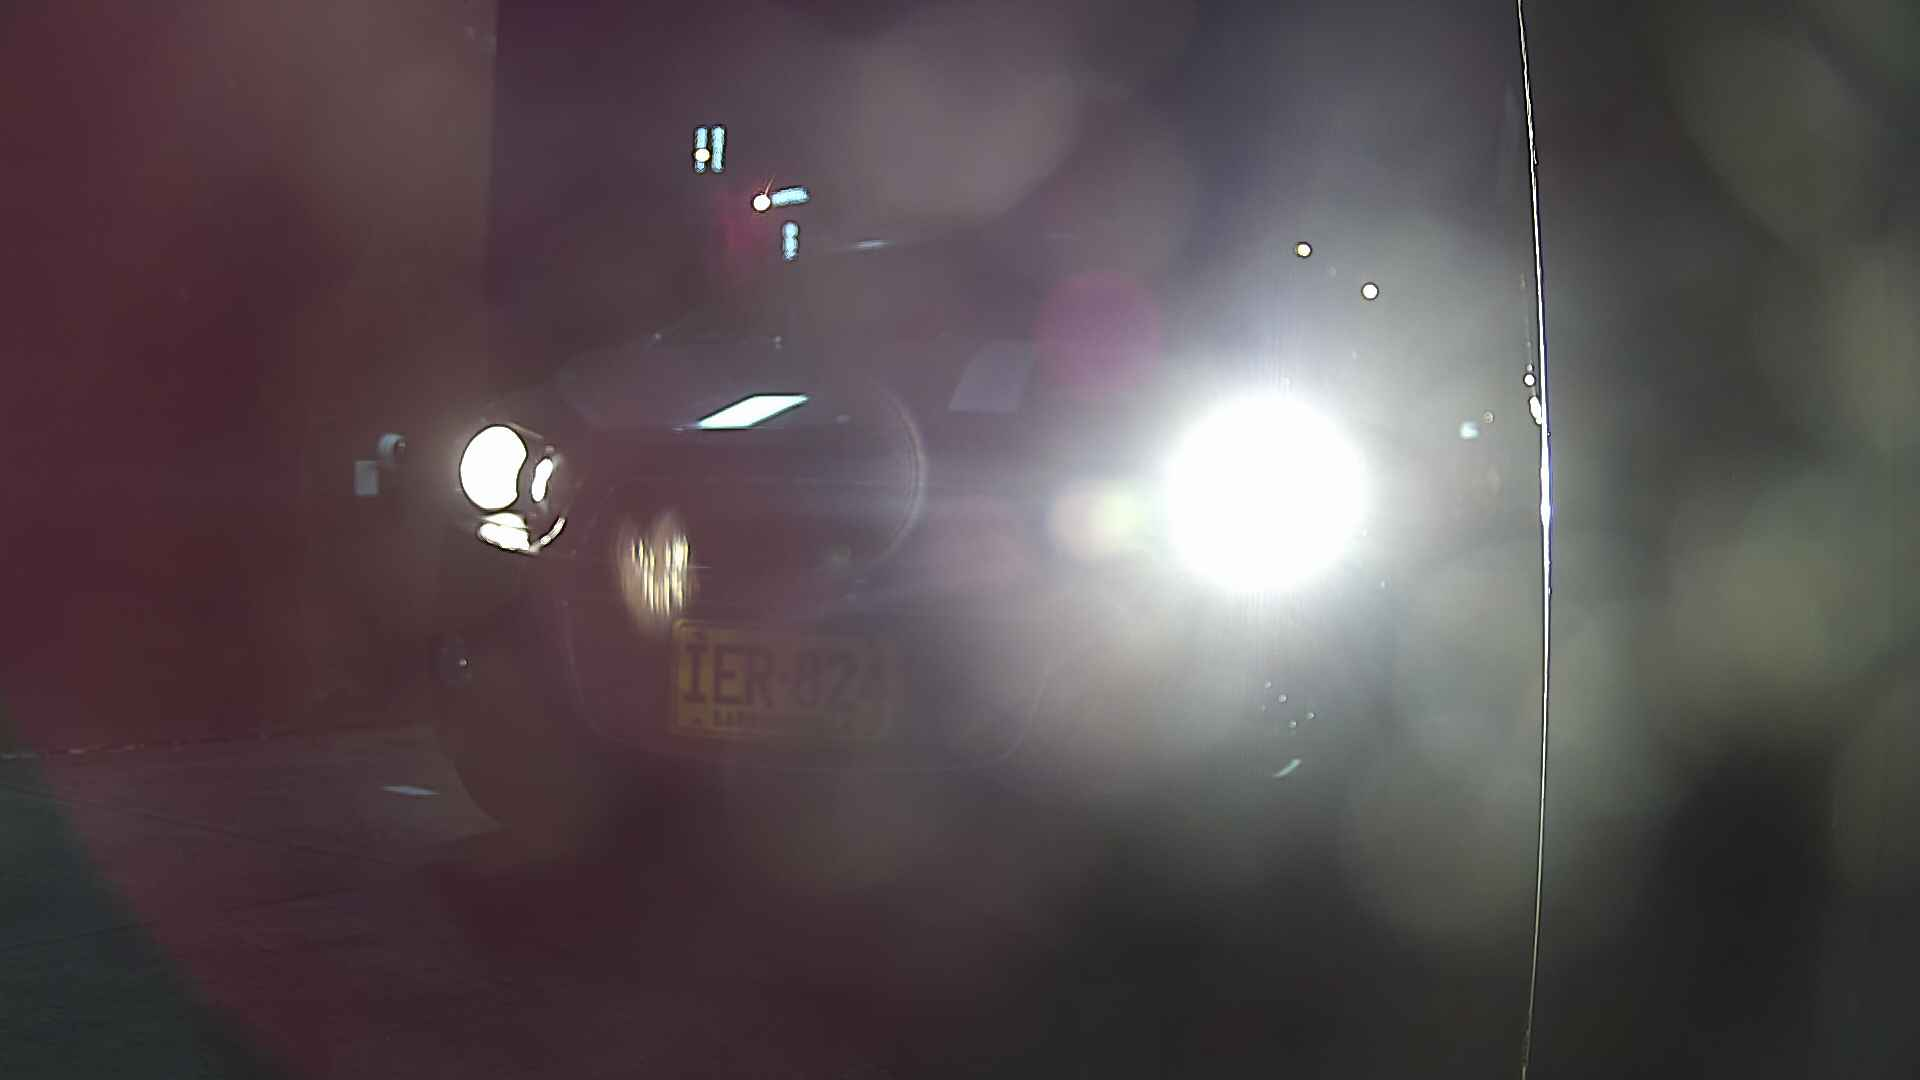
\includegraphics[width=0.8 \linewidth]{imagenes/Deterioradas/2018-11-04_17-57-36.jpg}}
    \caption{Placa de automóvil con condiciones adversas de iluminación}
    \label{fig:adversas} 
\end{center}
\end{figure}  
%-------------------------------
\item Reconocer las placas en diferentes perspectivas y escalamiento; 
    %--------------------------
    \begin{figure}[H]
\begin{center}
      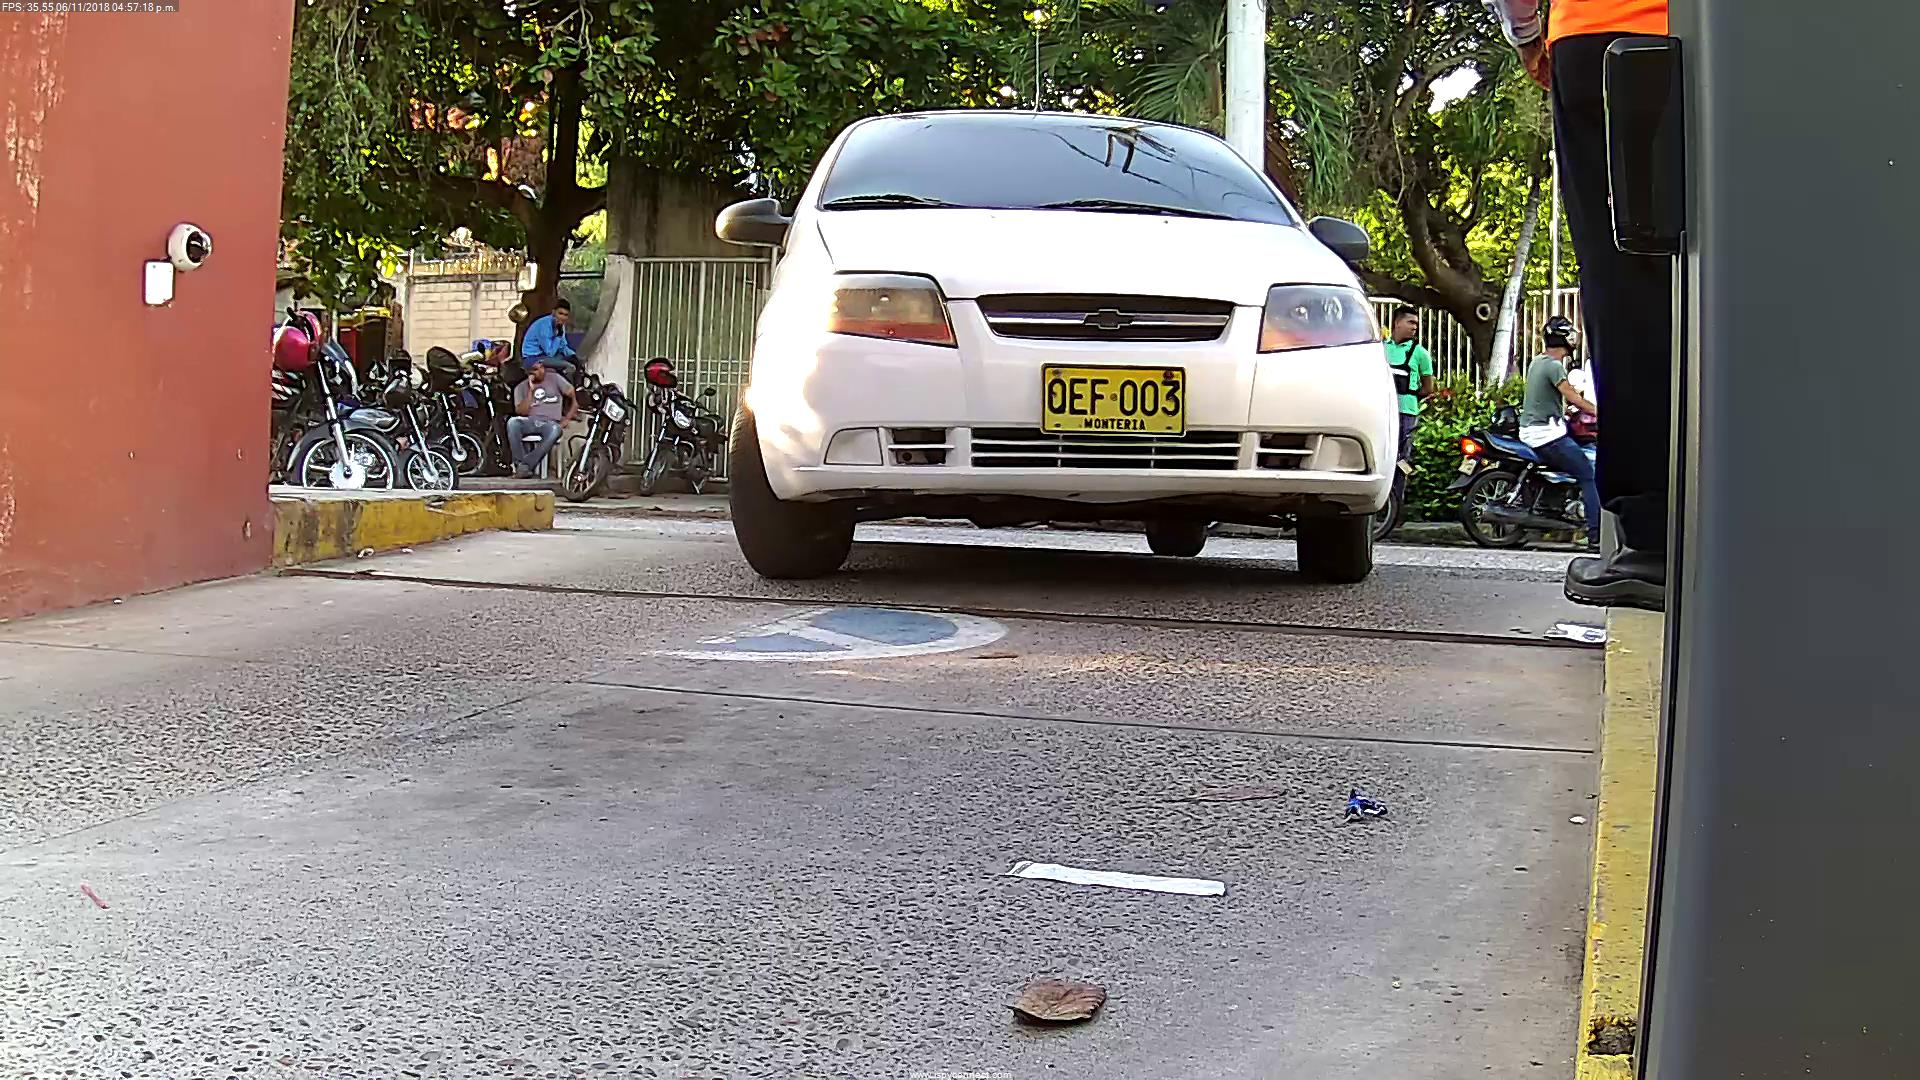
\includegraphics[width=0.8 \linewidth]{imagenes/Deterioradas/lejos.jpg}\\
    \caption{Placas con perspectiva lejana}
    \label{fig:lejos}  
\end{center}
\end{figure}
    %-----------------------
    \item Discriminar caracteres diferentes, pero con forma similar, tal como lo muestra la figura \ref{fig:similar};
    \end{enumerate}
 %--------------------
\begin{figure}[H]
\begin{center}
      \subfigure[]{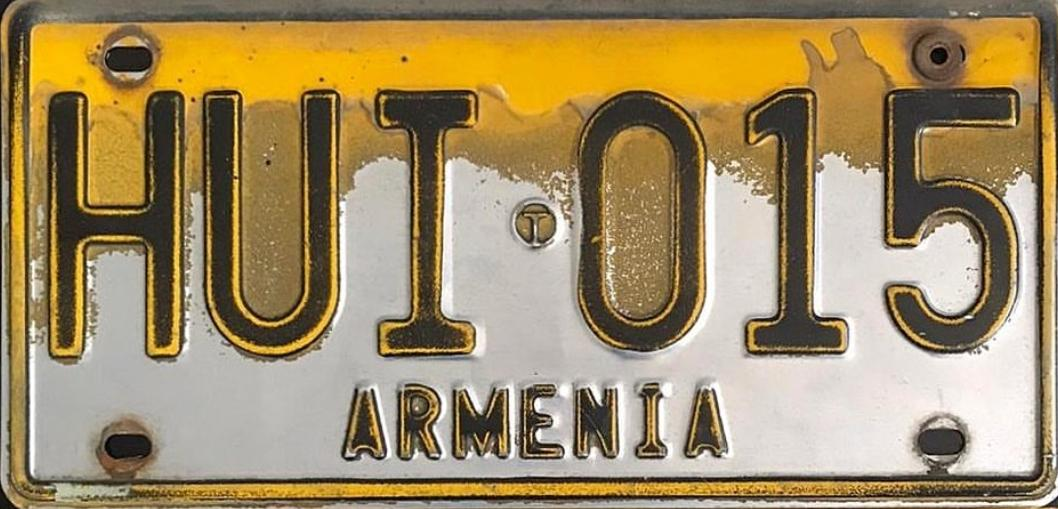
\includegraphics[width=0.4 \linewidth]{imagenes/Deterioradas/placa5.jpeg}}
    \subfigure[]{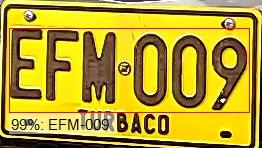
\includegraphics[width=0.35 \linewidth]{imagenes/Deterioradas/placa9.jpg}}
    \caption{Placas con caracteres similares: (a) letra I similar al número 1, (b) Letra E similar a la letra F}
    \label{fig:similar}  
\end{center}
\end{figure}
%------------------------------
   Para superar los retos planteados en el problema, nosotros proponemos usar Redes Neuronales Convolucionales, ya que son las ideales para el reconocimiento de objetos a partir de imágenes con demasiada variabilidad. Además, tales redes tienen incorporado una etapa de extracción de características que evitan su extracción manual que se realiza en el aprendizaje supervisado, para el posterior entrenamiento de una red neuronal convencional. El uso de RNC plantea unos retos técnicos, tales como: 
\begin{enumerate}
\item Conseguir una base de datos con placas colombianas debidamente etiquetada que permita el entrenamiento de la red; 
\item Escoger la mejor arquitectura de red que logre un excelente rendimiento.  
\end{enumerate}
%\newpage
\section{Pregunta de Investigación}

De acuerdo a los retos anteriormente planteados, la siguiente investigación trató de dar respuesta a las siguientes preguntas:

\begin{itemize}
    \item[i.] ¿Es posible mejorar el rendimiento de una RNC agregándole imágenes de caracteres de la base de datos chars74k a una base de datos de imágenes de caracteres segmentados de placas colombianas?
    \item[ii.]¿Qué tan experto es un sistema de reconocimiento de placas usando detección de objetos con redes neuronales mucho más rápidas, (Faster R-CNN)?
   
\end{itemize}

\section{Objetivo General}
Diseñar y elaborar un sistema experto para el reconocimiento de placas de automóviles en Colombia usando Redes Neuronales Convoluciones.
\section{Objetivos específicos}
\begin{itemize}
    \item Explorar y estudiar diferentes arquitecturas de RNC y las herramientas computacionales más usadas para su entrenamiento.

    \item Diseñar y construir una base de datos con imágenes de placas de automóviles en Colombia con alta variabilidad, para el entrenamiento y test de una  Red Neuronal Convolucional.

    \item Plantear una nueva arquitectura de RNC con alto rendimiento en el reconocimiento de placas de automoviles colombianas.
    
    \item Construir una base de datos con las coordenadas de caracteres de placas colombianas obtenidas usando Cuadros Delimitadores  (Bonding  Boxing) para entrenar una  Red  Neuronal  Convolucional mucho mas Ŕapida con propuesta de Regiones (Faster R-CNN). 
    
\end{itemize}

%-----------------------
\chapter{Marco teórico}\label{marcoteorico}
\section{Antecedentes}\\ \label{sec:antecendentes}

El reconocimiento automático de placas vehiculares es muy importante en los sistemas de control de tránsito. Estos sistemas implementan algoritmos que permiten analizar imágenes digitales utilizando técnicas de reconocimiento óptico de caracteres (del inglés, \textit{Optical character recognition} - OCR) \cite{noaman2012optical}. Para lograr esto, se usa con frecuencia la implementación de inteligencia artificial, que puede incluir componentes como redes neuronales, algoritmos genéticos, lógica difusa u ordenamiento estadístico \cite{Calderon2017}. En muchos países se realiza el reconocimiento automático de placas vehiculares para el acceso al estacionamiento, rastreo de vehículos, control de fronteras, conteo de vehículos e identificación policial con fines de seguridad. Esto ha sido fruto de algunas de las siguientes investigaciones: 

\begin{itemize}
    \item Patel et \textit{al} \cite{patel2013automatic} proponen un sistema con técnicas de aprendizaje supervisado en redes neuronales artificiales convolucionales, utilizando la plataforma Caffe y sus librerías, así como también librerías en OpenCV y scripts desarrollados en Python.
    \item Shivakumara et \textit{al} \cite{shivakumara2018cnn} combinaron CNN y RNN para reconocer imágenes de matrículas mediante clasificación. Para la clasificación de imágenes de matrículas privadas y públicas, el método propuesto exploró la separación de primer plano y fondo, y luego la agrupación de una nueva manera. Los resultados experimentales en la clasificación mostraron que la clasificación propuesta es mejor que los métodos existentes en términos de tasa de clasificación.
    \item En México se tienen estudios similares desde el año 2010 con el proyecto de Montiel et \textit{al} \cite{montiel2010reconocimiento}. Este autor propuso un sistema de reconocimiento de placas de los vehículos en la ciudad de México usando RNC. Los resultados experimentales obtenidos en condiciones reales de operación muestran que el sistema propuesto presenta un acierto del 99.84\% con caracteres que se usaron en el proceso de entrenamiento y un 98.78\% con caracteres que no fueron utilizados en el proceso de entrenamiento.
    \item Cika et \textit{al} \cite{cika2011detection} y Patel et \textit{al} \cite{patel2013automatic} usan algoritmos de segmentación múltiple para la identificación de la placa del vehículo, esto implica el uso doble de carga computacional, debido a que la comparación de patrones se usa en orden para dividir el área de la placa y paralela a esta, luego se implementan redes neuronales para identificar a cada personaje.
    \item Chu et \textit{al} \cite{chu2019sistema} implementaron un sistema de reconocimiento de placas vehiculares en un hospedaje ``Suites Recreo - 2019”\ en Perú. Se usó la metodología de desarrollo XP utilizando el algoritmo Clasificador Haar Cascade, motor de reconocimiento de caracteres Tesseract, librerías de visión artificial Opencv, EmguCV y Aforge.NET, el sistema gestor de base datos Mysql y el entorno de desarrollo Visual Studio 2015. Se obtuvo que el tiempo promedio de registro de vehículos sin el sistema fue de 47.27 segundos y con el sistema implementado fue de 15.10 segundos.
    \item Espinoza et \textit{al} \cite{espinoza2015desarrollo} desarrollaron un sistema de reconocimiento de placas vehiculares mediante el análisis de imágenes digitales. El uso de la interfaz gráfica web presentó una tasa de reconocimiento del 91\%.
    \item Alvarez et \textit{al} \cite{alvarez2014analisis} diseñaron un sistema de reconocimiento de placas vehiculares que permitió identificar los vehículos que ingresan al parqueadero de la Universidad Politécnica Salesiana. Este proceso usó una cámara conectada al sistema de visión artificial. Presentó un 94\% de acierto en el reconocimiento de placas.
    \item En Perú, Rojas et \textit{al} \cite{rojas2017desarrollo}, desarrollaron sistema de reconocimiento de placas en \textit{JAVAanpr} y estudiaron su influencia en la detección de vehículos robados en la municipalidad San Isidro. Los autores indican que al realizar la búsqueda de vehículos robados con la policía por los medios tradicionales no se llega ni al 20\% de efectividad además de tener un alto costo operativo, sin embargo aplicando inteligencia artificial, la efectividad de este sistema es del 96\%. 
    \item Diferentes empresas e instituciones Ecuatorianas tienen un prototipo para el acceso vehicular, de esta manera reemplazan el operador humano que se encargaba de la vigilancia, esto mediante técnicas de visión artificial valiéndose de insumo los vídeos de vigilancia de acceso. Así como tienen software y hardware comerciales de reconocimiento de placas, como: Transcore, Intellisoft Parking, FxCAM, IBW2000, 3LPR.
\end{itemize}

Por otro lado, en Colombia contamos con muy pocas investigaciones en este tema, la mayoría son tesis de pregrado y postgrado, y no fueron implementados considerando los recursos físicos como la memoria RAM, la memoria no volátil o la capacidad de procesamiento limitado. A continuación se mencionan algunos de estos estudios: 

\begin{itemize}
    \item Estudiantes del programa de ingeniería electrónica de la Pontificia Universidad Javeriana, desarrollaron un software de demostración para el reconocimiento de caracteres impresos en Turbo C++ \cite{TrabajodeGrado2}y en 2005, fue desarrollado otro sistema en la plataforma Microsoft.net con base en las funciones y clases del conjunto de librerías Open source Computer Visión\cite{TrabajodeGrado}. Por su parte y como una iniciativa propia, la Universidad de los Andes desarrolló un sistema que utiliza sistemas de visión artificial para el tratamiento de imágenes con el fin de automatizar este proceso en sus instalaciones \cite{Uniandes}.
    \item González \& Col. (2008) crearon el software RAMVP V1.0 que trabaja con la plataforma MatLab. La investigación de estos autores combinaron distintos métodos de procesamiento de imágenes. El primero, extraía información de una escena paso a paso; y el segundo fue  una implementación preliminar de redes neuronales artificiales en el reconocimiento de patrones. Cientes de que puede abrir nuevos campos, el software creado trabaja con otro tipo de metodología\cite{trabajodegrado3}.
    \item Recientemente, Vasquez \& Melo (2018) diseñaron un sistema de conteo y reconocimiento automático de placas vehiculares, para el parqueadero de la sede principal de la Universidad Cooperativa de Colombia seccional Bogotá. También fue utilizado el software matemático MATLAB\cite{melo2019sistema}
    \item La investigación desarrollada por Calderón et \textit{al}\cite{Calderon2017} es el primero  en Colombia que propone abiertamente un reconocimiento del número de matrícula utilizando solo componentes de software. El sistema propuesto es integrado con recursos limitados y con capacidad de procesamiento mixto, específicamente usando el ZedBoard, que incluye un dispositivo Zynq 7000 Xilinx device. Es importante mencionar que Calderón et \textit{al}  \cite{Calderon2017} utiliza un método similar al propuesto en este trabajo. Sin embargo, los autores implementan una red neuronal poco compleja (capa de entrada: 128, capa oculta: 15 y capa de salida: 6 neuronas) programado en un sistema informático Linux, con costos computacionales relativamente altos (software y hardware), y una cámara estándar de detección.
\end{itemize}

\section{Marco conceptual}

Las competencias necesarias para llevar a cabo el presente trabajo, se relacionan con el campo del Deep Learning, específicamente todo lo relacionado con la comprensión de las Redes Neuronales Convolucionales. Desde como construir una arquitectura desde cero hasta la implementación de la transferencia de aprendizaje. Además, entender las diferentes métricas para evaluar su rendimiento. También, fue necesario adquirir competencias en las diferentes herramientas computacionales para su implementación. 
Por otro lado, para la construcción de la base de datos fue necesario entender algunas técnicas de segmentación y etiquetado propias del procesamiento de imágenes y conocer las herramientas computacionales para realizar tal tarea. 
El marco conceptual que se describe a continuación está relacionado con todos los conceptos básicos que permitieron adquirir todas las competencias antes mencionadas.

\subsection{Machine Learning}

Una regla de aprendizaje no es más que un procedimiento por el cual se modifican los pesos y el “bias” de la red. El propósito principal de que una red aprenda es que sea capaz de resolver una tarea que antes no podía (sabía) resolver. Existen muchos tipos de métodos de aprendizaje, pero los principales son: aprendizaje supervisado, aprendizaje no supervisado y aprendizaje reforzado\cite{Algoritmos}.

\begin{itemize}
    \item \textbf{Aprendizaje supervisado}: El aprendizaje se realiza mediante un entrenamiento controlado por un agente externo (supervisor, maestro) que determina la respuesta que debería generar la red a partir de una entrada determinada. El supervisor controla la salida de la red y en caso de que esta no coincida con la deseada, se procederá a modificar los pesos de las conexiones, con el fin de conseguir que la salida obtenida se aproxime a la deseada. Para lograr lo anterior, la red es provista con una seria de ejemplos que indican como la red debe funcionar.
    \item \textbf{Aprendizaje reforzado}: La diferencia con el caso anterior, es que cada entrada está asociada a una puntuación. Esta puntuación es una medida del rendimiento de la red ante varias secuencias de entrada. Dependiendo de la nota, la red actuará de una manera u otra: sí la nota es baja, el algoritmo de aprendizaje modificará en gran medida los elementos de la matriz de pesos y el bias, si la nota es media, los modificará más suavemente, y si es buena, los mantendrá o apenas modificará.
    \item \textbf{Aprendizaje no supervisado}: Son aquellos en los que no disponemos de una batería de ejemplos previamente clasificados, si no que la matriz de peso y el bias son modificadas en respuesta solo a las entradas de la red, ya que no existen objetivos. De esta manera, los algoritmos trabajan agrupando, es decir, la red aprende a categorizar los patrones de entrada en una serie finita de clases, según las propiedades de los ejemplos buscando la similitud.
\end{itemize}

\subsubsection{Algoritmo de aprendizaje supervisado \textit{backpropagation}}

El algoritmo de aprendizaje de estas redes permite extraer los atributos o características de cada clase a partir de un conjunto de datos de entrenamiento previamente clasificado. Estos atributos son los pesos de las diferentes neuronas de la red, y sus valores se calculan de manera iterativa mediante un método de aprendizaje supervisado denominado backpropagation o “propagación de errores hacia atrás”\cite{lecun1989backpropagation,chauvin1995backpropagation}. El algoritmo consta de dos etapas que se repiten interactivamente por cada elemento del conjunto de entrenamiento \cite{hecht1992theory}:
\begin{itemize}
    \item Etapa 1: Se calcula la clase a la que pertenece el ejemplar de entrada según los valores actuales de los pesos de la red. Una vez clasificado, el algoritmo determina la validez de dicha clasificación mediante una función de error.
    \item Etapa 2: El algoritmo propaga el error hacia atrás a todas las neuronas de la red que han contribuido a la clasificación del ejemplar, recibiendo cada una la “porción” del error correspondiente en función de su aportación, para que actualicen los pesos proporcionalmente, de tal manera que los nuevos valores reduzcan el error de clasificación. 
\end{itemize}
El algoritmo empleado para esta optimización suele ser el de descenso del gradiente. La combinación de ambos métodos; propagación hacia atrás y descenso del gradiente tiene como objetivo minimizar la función de error \cite{marin2013introduccion}.

\subsection{Redes Neuronales Artificiales - RNA}

Las redes neuronales biológicas son inmensas redes de neuronas interconectadas mediante procesos químicos y eléctricos. Todas esas neuronas conectadas entre sí le permiten al ser humano ser capaz de sentir, memorizar, aprender, etc. las redes neuronales artificiales (RNA) o perceptrón surgen del intento de imitar el comportamiento de las neuronas cerebrales usando software y hardware ultra avanzados \cite{marin2013introduccion}. Las características principales de las RNA son las siguientes:

\begin{itemize}
    \item Auto-Organización y Adaptabilidad: Utilizan algoritmos de aprendizaje adaptativo y auto-organización, por lo que ofrecen mejores posibilidades de procesado robusto y adaptativo.
    \item Procesado no Lineal: Aumenta la capacidad de la red para aproximar funciones, clasificar patrones y aumenta su inmunidad frente al ruido. 
    \item Procesado Paralelo: Normalmente se usa un gran número de nodos de procesado, con alto nivel de interconectividad.
\end{itemize}

Las RNA consisten de un gran número de elementos simples de procesamiento llamados nodos o neuronas que están organizados en capas. Cada neurona está conectada mediante enlaces de comunicación, cada uno de los cuales tiene asociado un peso. Estos pesos representan la información que será usada por la red neuronal para resolver un problema determinado, Matich et \textit{al} \cite{matich2001redes}.\\ 

\begin{figure}[H]
    \centering
    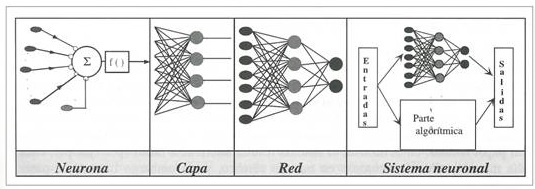
\includegraphics[width=1\linewidth]{imagenes/perceptron.jpg}
    \caption{Estructura jerárquica de una red neuronal artificial (RNA)}
    \label{fig:Estructura jerárquica de una red neuronal artificial (RNA)}
\end{figure}

\textbf{La figura \ref{fig:Estructura jerárquica de una red neuronal artificial (RNA)}} nos muestra en detalle cada elemento que forma a una RNA, una neurona, la capa, la red y todo el sistema conformado por cada uno de estos elementos. Hay tres fases en la modelización con redes neuronales \cite{marin2013introduccion}:

\begin{itemize}
    \item \textbf{Fase de entrenamiento}: Se usa un conjunto de datos para determinar los pesos que definirán el modelo de la red neuronal.
     \item \textbf{Validación}: Para evitar el problema del sobreajuste, se usa un conjunto de datos diferentes a los de entrenamiento, el grupo de validación, que permita controlar el proceso de aprendizaje.
    \item \textbf{Fase de Prueba}: En la fase anterior, el modelo puede que se ajuste demasiado a las particularidades presentes en los patrones de entrenamiento, perdiendo su habilidad de generalizar su aprendizaje a casos nuevos (sobreajuste).
\end{itemize}    
Usualmente con una única neurona no será suficiente para resolver la mayoría de problemas prácticos. Para resolver problemas más complejos se tendrá que hacer un uso conjunto de muchas de estas neuronas simples, dando lugar a una verdadera red neuronal, en la que se tendrán cientos o incluso miles de neuronas. Es ahí donde aparece el concepto de capa, que es la agrupación de todas estas neuronas en varios conjuntos dentro de la red neuronal completa \cite{duran2017redes}. 
    
\begin{figure}[H]
\centering
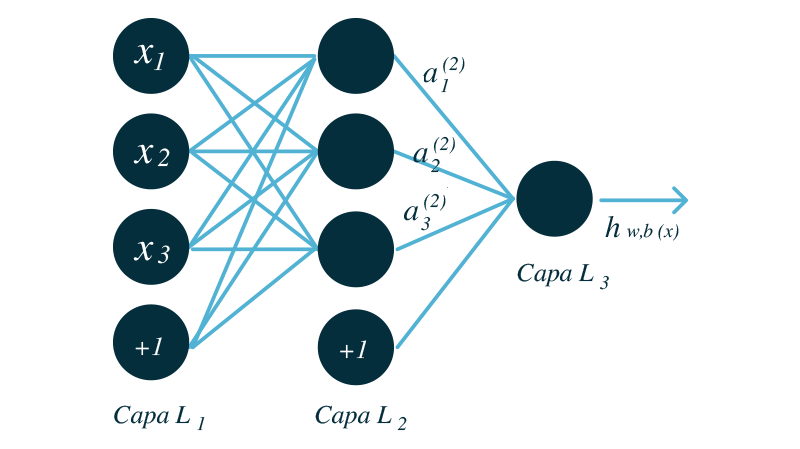
\includegraphics[width=0.7\linewidth]{imagenes/3_capas.png}
\caption{Estructura de una red neuronal de 3 capas}
\label{fig:3_CAPAS}
\end{figure}

La figura \ref{fig:3_CAPAS} es una muestra de una red neuronal artificial con una sola capa oculta, una de entrada y una capa de salida, para conformar así, 3 capas en sus sistema neuronal.\\
Si tenemos $n_{l}$ capas en una red neuronal, la l-ésima capa se denominará $L_{l}$, en ese sentido, la capa de entrada de la red será $L_{1}$, así mismo la capa de salida de la red será $L_{n}__{l}$. También se tendrá que $W_{ij}^{l}$ será el peso asociado a la conexión entre el elemento j de la capa l y el elemento i de la capa l+1, además, es la bias $b_{i}^{l}$ asociada con el elemento i de la capa l+1. Por último, se usará $a_{i}^{l}$ para denotar la activación (es decir, el valor de salida) del elemento i en la capa l. \\
El vector de entrada \textbf{X} está conectado con cada una de las
neuronas a través de la matriz de pesos \textbf{W}, es decir cada neurona de cada capa está conectada con todos los elementos de la capa que le precede. Este tipo de capas se denomina totalmente conectada o, en inglés, full connected. Además, cada neurona posee su propia bias. Todo esto supone que la salida de la neurona $n_{i}$ vendrá dada por la suma ponderada entre cada elemento de la entrada multiplicado por su correspondiente elemento de la matriz de pesos y la bias, en otras palabras, es:
\begin{center}
    $a_{1}^{2}= f({W_{11}^{1}X_{1}+W_{12}^{1}X_{2}+W_{13}^{1}X_{3}+b_{1}^{1}})$
    $a_{2}^{2}= f({W_{21}^{1}X_{1}+W_{22}^{1}X_{2}+W_{23}^{1}X_{3}+b_{2}^{1}})$
    $a_{3}^{2}= f({W_{31}^{1}X_{1}+W_{32}^{1}X_{2}+W_{33}^{1}X_{3}+b_{3}^{1}})$
    $h_{w,b}(X)=a_{1}^{3}= f({W_{11}^{2}a_{1}^{2}+W_{12}^{2}a_{2}^{2}+W_{13}^{2}a_{3}^{2}+b_{1}^{3}})$
\end{center}
    
Donde $h_{w,b}(X)$ es la salida de la red neuronal. ver figura\ref{fig:3_CAPAS}

\subsection{Deep Learning (Aprendizaje Profundo)}

El aprendizaje profundo, del inglés \textit{Deep Learning}, es una rama del aprendizaje automático (\textit{Machine Learning}), ambas se consideran dos subcategorías de la IA. \textit{Deep Learning} está basada en un conjunto de algoritmos que intentan modelar abstracciones de alto nivel usando un gráfico profundo con varias capas de procesamiento, compuesto de varias transformaciones lineales y no lineales \cite{bengio2017deep}.

Se han aplicado diversas arquitecturas de aprendizaje profundo, Bengio et \textit{al} \cite{bengio2009learning}, como: redes neuronales profundas, redes neuronales convolucionales profundas, redes de creencias profundas y redes neuronales recurrentes en áreas como:
\begin{itemize}
    \item Clasificación de imágenes a nivel casi humano.
    \item Reconocimiento de voz a nivel casi humano.
    \item Transcripción de escritura a mano a nivel humano.
    \item Mejora de la traducción automática.
    \item Mejora de la conversión de texto a voz.
    \item Asistentes digitales como Google Now o Amazon Alexa.
    \item Conducción autónoma a nivel humano.
    \item Mejora de la orientación de anuncios.
    \item Mejora de los resultados de búsqueda en la web.
    \item Responder preguntas de lenguaje natural.
\end{itemize}

\subsubsection{Redes Neuronales Convolucionales - RNC} \label{sec:RNC}

Las redes neuronales convolucionales son un tipo de RNA con aprendizaje supervisado que procesa sus capas imitando el córtex visual del ojo humano para identificar distintas características en la entrada que permiten la identificación de objetos, Erroz et \textit{al} \cite{erroz2019visualizando}. Las tareas principales que realizan las RNC son:
\begin{itemize}
    \item Detección/categorización de objetos
    \item Clasificación de escenas
    \item Clasificación de imágenes en general
\end{itemize}

\begin{figure}[H]
    \centering
    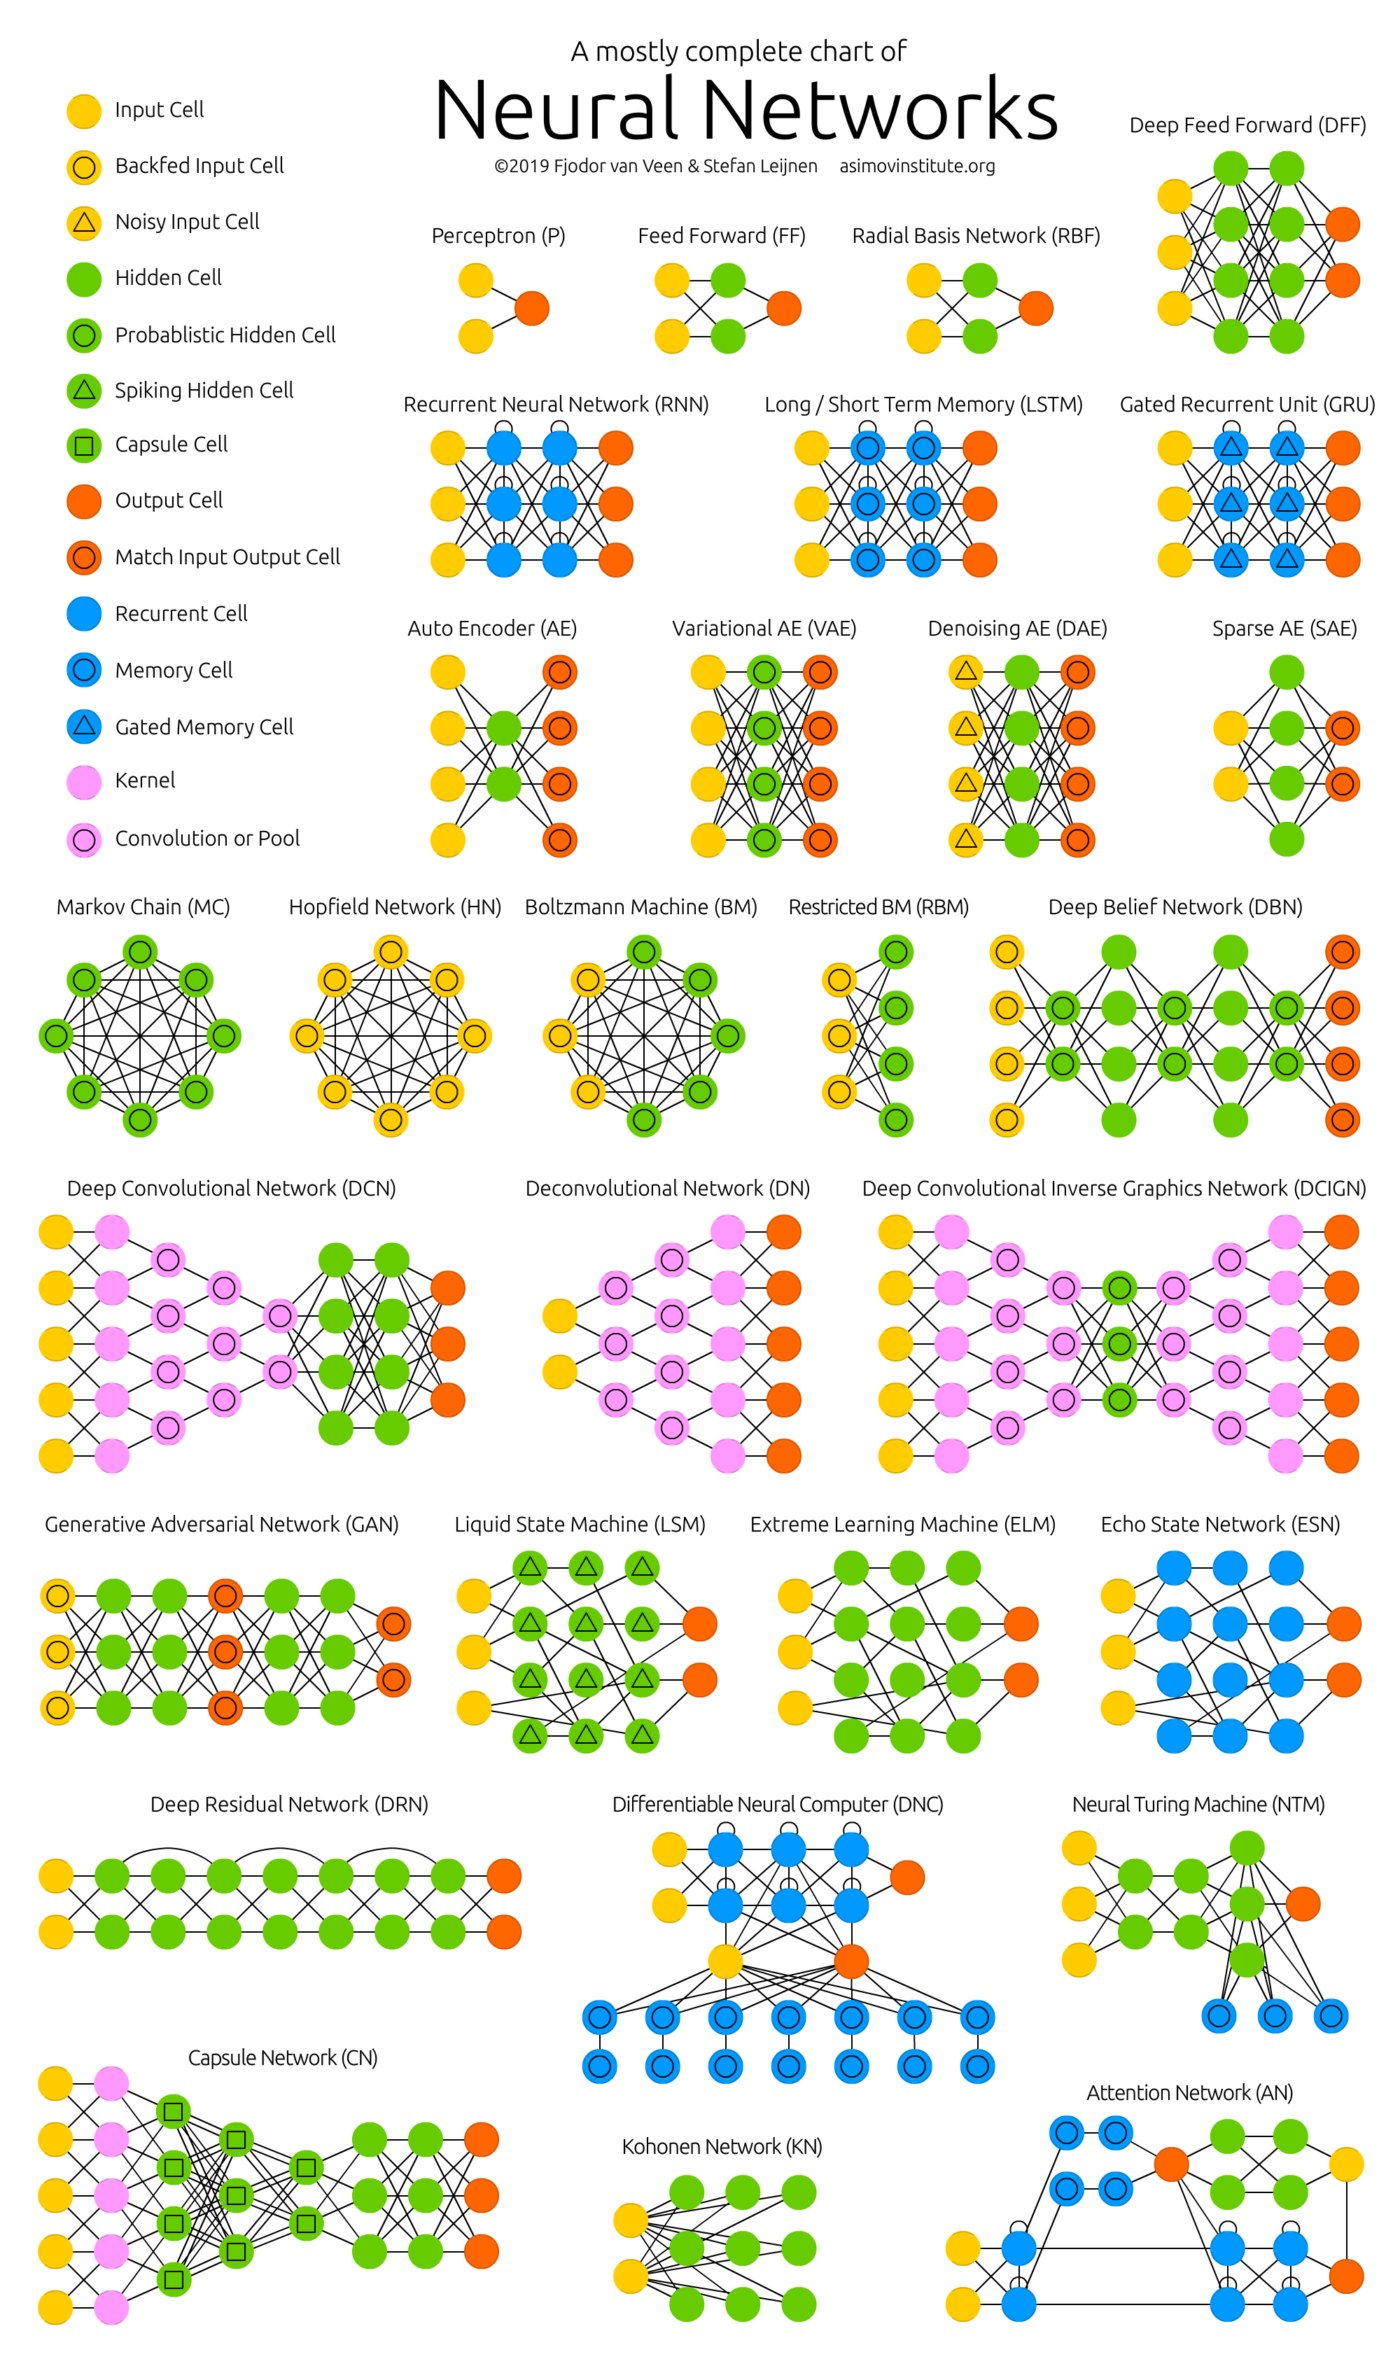
\includegraphics[width=0.7\linewidth]{imagenes/NeuralNetworkZoo20042019-1400x2380.png}
    \caption{Tipos de redes neuronales. \textit{Tomado de ASIMOV INSTITUTE about The Neural Network Zoo}
    \label{fig:my_Label})}
\end{figure}


Una red neuronal convolucional consta de diversas capas convolucionales y de pooling (submuestreo) alternadas, y al final tiene una serie de capas full-connected como una red perceptron multicapa. La entrada de una red capa convolucional suele ser, generalmente, una imagen m	x	m	x	r, donde m es tanto la altura como el ancho de la imagen y r es el número de canales. Las capas convolucionales tienen K filtros (o
kernels) cuyas dimensiones son 	n x n x q, donde n y q son elegidas por el diseñador (generalmente q suele ser igual a r). Cada filtro genera mediante convolución un mapa de rasgos o características de tamaño (m-n+1) x (m-n+1) x p, siendo p el número de filtros que se desean usar. Después cada mapa es sub-muestreado en la capa de pooling con la operación “mean pooling” o “max pooling” sobre regiones contiguas de tamaño p x p, donde p puede tomar valores desde 2 para imágenes pequeñas hasta,comúnmente, no más de 5 para imágenes grandes. Antes o después del submuestreo, se aplica una función de activación sigmoidal más un sesgo para cada mapa de rasgos \cite{duran2017redes}.

\subsection {Estructura de una Red Neuronal Convolucional}

La estructura más sencilla de una RNA se conforma de tres capas, una capa de entrada, una capa oculta y una capa de salida, donde cada neurona de una capa se conecta a todas las neuronas de la otra, conocido como \textit{Fully Connected}. En una RNC, cada capa es un bloque con tres principales variables: entrada, pesos y salida. La característica fundamental es que la salida de una capa se convierte en la entrada de la próxima, es decir, se comparten las neuronas a través de filtros que permiten extraer información de las imágenes de entrada. Este proceso es secuencial y puede ser no lineal, en cada capa se realiza una función específica \cite{lecun1998gradient}.

\begin{itemize}

\item \textbf{Capa de entrada:} La capa de entrada en una red neuronal convolucional es la imagen de la base de datos que usaremos para el entrenamiento. 

\begin{figure}[H]
    \centering
    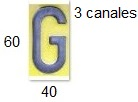
\includegraphics[width=0.4\linewidth]{imagenes/imagen_entrada.jpg}
    \caption{Imagen entrada red neuronal convolucional
    \label{fig:imagen_entrada}}
\end{figure}

\item \textbf{Capa convolucional:}Esta capa es el núcleo de las redes neuronales convolucionales. Los parámetros de esta capa consisten en un conjunto de filtros de aprendizaje, los cuales tiene un campo receptivo muy pequeño. En el paso hacia delante de aprendizaje, cada filtro se convoluciona con todo el campo de visión produciendo un mapa de características. Cada elemento del mapa de características puede interpretarse como la salida de una neurona que extrae información de una pequeña región de la entrada y comparte parámetros con neuronas que se encuentran en el mismo mapa \cite{bouvrie2006notes}. En general, el mapa de características de una capa está dado por: 

\begin{center}
    $Y_{j}^l = f(\sum_{i\in M_{j}}y_{i}^{l-1}k_{ji}^{l-1} + b_{j})$
\end{center}

Donde $M_{j}$ representa el conjunto de entradas seleccionadas y el superíndice l representa la capa actual. Cada mapeo de salida tiene un sesgo diferente. La convolución proporciona facilidad para trabajar con entradas de tamaño variable.    

La ventaja es que el mismo filtro sirve para extraer la misma característica en cualquier parte de la entrada, con esto que consigue reducir el número de conexiones y el número de parámetros a entrenar en comparación con una red multicapa de conexión total.

La fase convolucional aplicar\'a un filtro que es una pequeña matriz de píxeles dentro de la imagen. El filtro se moverá a lo largo y ancho de la imagen de entrada con dimensiones comúnmente de 3 x 3 o 5 x 5. Significa que la red desliza estas ventanas a través de toda la imagen de entrada y calcula la convolución que da como resultado una matriz que se denomina mapa de características.

\begin{figure}[H]
\centering
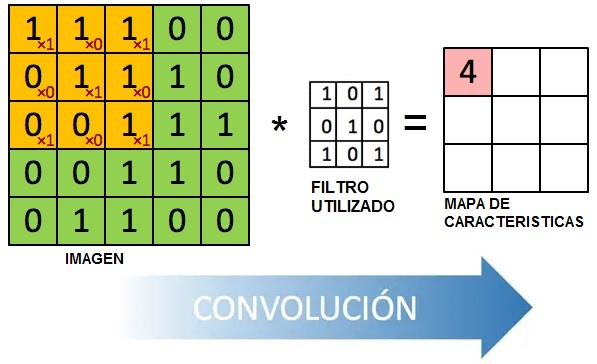
\includegraphics[width=0.5\linewidth]{imagenes/OPERACION_1.jpg}
\caption{Operación convolución}
\label{fig:OPERACION_1}
\end{figure}

En la figura \ref{fig:OPERACION_1} se ha tomado una submatriz de la imagen de entrada, con unas dimensiones igual al filtro, es decir, 3 x 3, donde las componentes son $X_{11}, X_{12}, X_{13}, X_{21}, X_{22}, X_{23}, X_{31}, X_{32}, X_{33}$ que se operan con el filtro, de la siguiente forma: $(1\times1) + (1\times0) + (1\times1) + (0\times0) + (1\times1) + (1\times0) + (0\times1) + (0\times0) + (1\times1) = 4 $ el filtro se desplaza en toda la imagen y obtenemos el mapa de características, así: 

\begin{figure}[H]
\centering
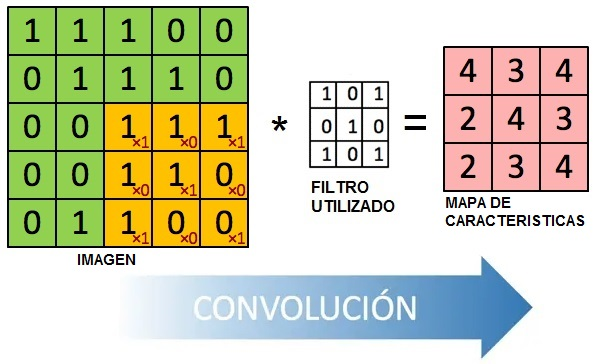
\includegraphics[width=0.4\linewidth]{imagenes/OPERACION_2.jpg}
\caption{Operación convolución}
\label{fig:OPERACION_2}
\end{figure}

\textbf{En la figura \ref{fig:OPERACION_2}} muestra como se obtiene la última componente del mapa de características, haciendo uso de $X_{33}$, $X_{34}$, $X_{35}$, $X_{43}$, $X_{44}$, $X_{45}$, $X_{53}$, $X_{54}$, $X_{55}$ de la imagen,  operado con el filtro, así: $(1\times1) + (1\times0) + (1\times1) + (1\times0) + (1\times1) + (0\times0) + (1\times1) + (0\times0) + (0\times1) = 4 $ se debe resaltar que después de esta operación el tamaño de la imagen de entrada se reduce.


En este trabajo haremos uso de imágenes de 1 y 3 canales(RGB), donde el proceso de convolución es diferente, puesto que se hace uso de los 3 filtros o kernel a la vez, en la figura \ref{fig:OPERACION1_3_CANALES} ilustramos este procedimiento.

\begin{figure}[H]
\centering
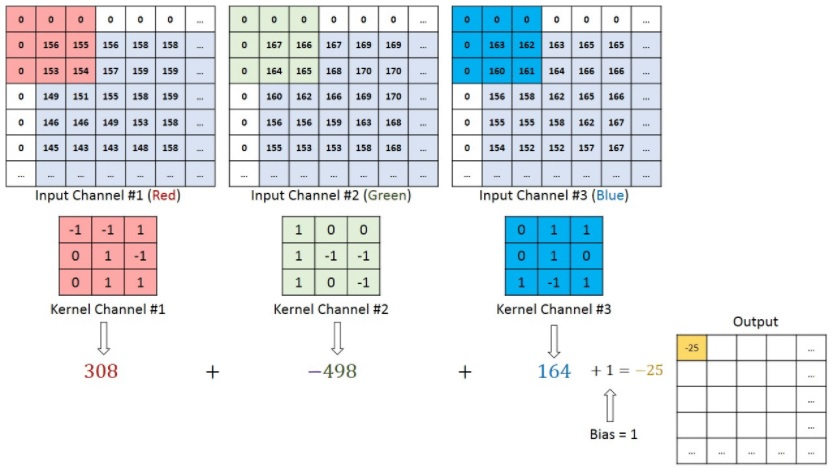
\includegraphics[width=0.8\linewidth]{imagenes/OPERACION1_3_CANALES.jpg}
\caption{Operación convolución con 3 canales RGB}
\label{fig:OPERACION1_3_CANALES}
\end{figure}
\textbf{La figura \ref{fig:OPERACION1_3_CANALES}} representa las 3 matrices para cada uno de los canales de una imagen RGB, donde se aplicada la operación de convolución con 3 filtros, donde los resultados son sumados entre si, anexando el bias.

Es importante tener en cuenta, que la imagen de salida al aplicar el filtro se reduce, comúnmente a partir del Stride con zancada 1, que tiene que ver con el desplazamiento que tiene el filtro en la matriz de entrada, si la zancada es dos, se moverá cada 2 píxeles y así sucesivamente, si queremos que la imagen de salida permanezca con los mismo píxeles de entrada, debemos hacer uso del relleno que resuelve este problema, Ren et \textit{al} \cite{Ren_2017}.

\begin{figure}[H]
\centering
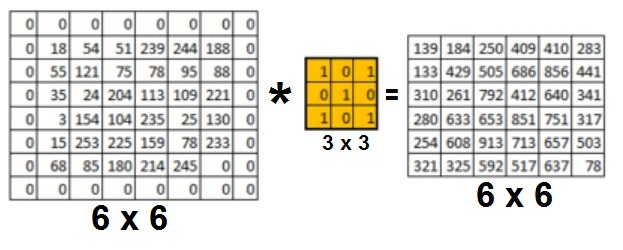
\includegraphics[width=0.5\linewidth]{imagenes/relleno.jpg}
\caption{Relleno}
\label{fig:RELLENO}
\end{figure}

\item \textbf{Capa ReLu:} El objetivo en esta capa es introducir la no linealidad, lo que significa que podemos propagar fácilmente los errores hacia atrás y tener múltiples capas de neuronas activadas por la función ReLU en nuestra red, Shaoqing et \textit{al} \cite{DBLP:journals/corr/RenHG015}. Esta función de activación se define como:\\  

R(Z) = max(0,z) = $\bigl\{\begin{array}{ccc}
    0 & para & Z<0\\
    Z & para & Z\geq 0
\end{array}$ , gráficamente es:

\begin{figure}[H]
\centering
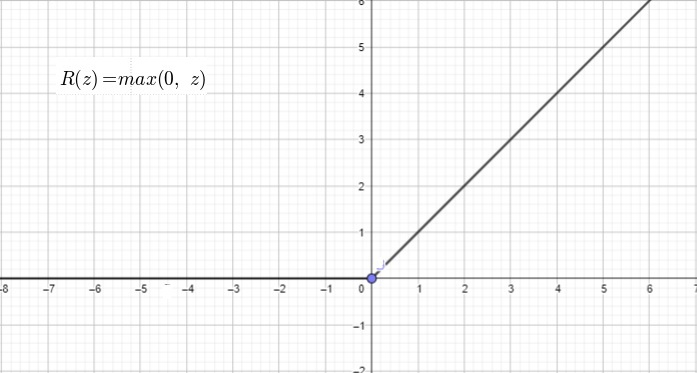
\includegraphics[width=0.7\linewidth]{imagenes/funcion_Relu.jpg}
\caption{Función de activación ReLu}
\label{fig:función_relu}
\end{figure}

Esta función se usa para permitir la no linealidad, en este componente se reemplazan los valores negativos de los píxeles por cero, tal y como se muestra en la figura \ref{fig:Relu}

\begin{figure}[H]
\centering
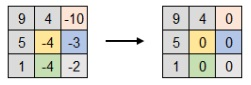
\includegraphics[width=0.7\linewidth]{imagenes/Relu.jpg}
\caption{Aplicación de la función de activación ReLu}
\label{fig:Relu}
\end{figure}

\item \textbf{Capa de submuestreo:} Se coloca después de la primera capa convolucional-ReLu con el fin de disminuir el tamaño de los datos. La operación que se realiza es mean-pooling(AVEPOOL) o comúnmente max-pooling de dimensión $s_{2}$, esta última tiene una salida:

\begin{center}
 $Y_{h}^{l} = Maxpool(Y_{h}^{l-1},s_{2} )$   
\end{center}

Esta capa reduce la cantidad de información que la capa convolucional generó para cada característica y mantiene la información más esencial (el proceso de las capas convolucionales y de agrupación generalmente se repite varias veces) \cite{pacheco2017identificacion}.

\begin{figure}[H]
\centering
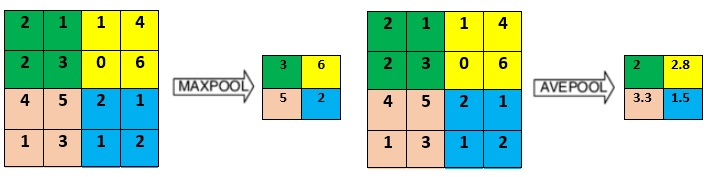
\includegraphics[width=0.7\linewidth]{imagenes/maxpooling.jpg}
\caption{Operación de max-pooling y de average-pooling}
\label{fig:Maxpooling}
\end{figure}

\textbf{La figura \ref{fig:Maxpooling}} evidencia la operación maxpooling y la operación average-pooling, la primera consiste en elegir de las componentes $X_{11}$, $X_{12}$, $X_{21}$, $X_{22}$, el máximo valor, en ese caso escogemos la componente $X_{22}$, lo mismo sucede con las componentes $X_{13}, X_{14}, X_{23}, X_{24}$ se escoge la componente $X_{24}$ ,así hacemos hasta completar las cuatro componentes del filtro 2 x 2, teniendo en cuenta que la imagen de entrada es de 4 x 4 píxeles y aplicamos un stride 2. Averagepooling consiste en hallar en este caso el promedio de las 4 componentes agrupadas anteriormente, a diferencia del máximo valor como en el caso antes mencionado. 

\item Capa de entrada totalmente conectada: “aplana” las salidas generadas por las capas anteriores para convertirlas en un solo vector que se puede usar como entrada para la siguiente capa.
\item Capa totalmente conectada: aplica pesos sobre la entrada generada por el análisis de características para predecir una etiqueta precisa.


\item \textbf{Capa Softmax o Rectified Lineal Unit:} La función Softmax transforma las salidas a una representación en forma de probabilidades para así determinar una clase para la imagen, la suma de todas las probabilidades de las salidas es igual 1.

La función esta definida como: $f(z)_j=\frac{e^{z_j}}{\sum\limits_{k=1}^{K}e^{z_k}}$, 
 donde \textit{Z} es una vector de entrada que arrojará por medio de la función de activación softmax las probabilidades para cada clase. En la figura \ref{fig:red_cov_digito_7} se resalta en un óvalo rojo la capa softmax con los valores entre 0-1 asignados a cada clase, donde la de mayor probabilidad pertenece a la clase 7.

\end{itemize}

\begin{figure}[H]
    \centering
    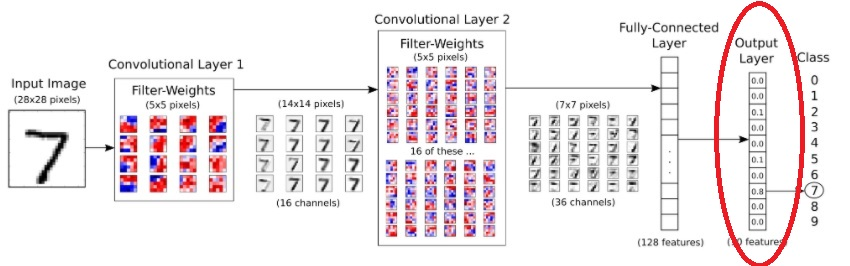
\includegraphics[width=1\linewidth]{imagenes/red_cov_digito_7.jpg}
    \caption{Arquitectura de una Red Neuronal Convolucional - RNC}
    \label{fig:red_cov_digito_7}
\end{figure}

La arquitectura de una RNC, figura \ref{fig:red_cov_digito_7} es un factor clave para determinar su rendimiento y eficiencia. La forma en que se estructuran las capas, qué elementos se usan en cada capa y cómo se diseñan a menudo afectará la velocidad y precisión con la que puede realizar diversas tareas.\\

\subsection{Evaluación del modelo de red neuronal convolucional}

\item \textbf{Matriz de confusión:} En el campo de la inteligencia artificial  y el aprendizaje automático una matriz de confusión es una herramienta que permite visualizar el desempeño de un algoritmo  de aprendizaje supervisado. Cada columna de la matriz representa el número de predicciones de cada clase, mientras que cada fila representa a las instancias en la clase real., o sea en términos prácticos nos permite ver  qué tipos de aciertos y errores está teniendo nuestro modelo a la hora de pasar por el proceso de aprendizaje con los datos, Danjuma et \textit{al} \cite{danjuma2015performance}

\begin{table}[H]
\begin{center}
\begin{tabular}{ll|c|c|}
\cline{3-4}
                   &  & \multicolumn{2}{c|}{\textbf{Categorías predichas}}\\\cline{3-4}
                                & \textbf{} & \textbf{Positivos} & \textbf{Negativos}                                                    \\ \hline 
      
\multicolumn{1}{|c|}{\multirow{2}{*}{\textbf{\begin{tabular}[c]{@{}c@{}}\\Categorías \\ verdaderas\end{tabular}}}} & \multicolumn{1}{c|}{\textbf{Positivos}} & \begin{tabular}[c]{@{}c@{}}Verdaderos\\ positivos\\ (VP)\end{tabular} & \begin{tabular}[c]{@{}c@{}}Falsos \\ negativos\\ (FN)\end{tabular}    \\ \cline{2-4} 
\multicolumn{1}{|c|}{}                                                                                           & \multicolumn{1}{c|}{\textbf{Negativos}} & \begin{tabular}[c]{@{}c@{}}Falsos\\ positivos\\ (FP)\end{tabular}     & \begin{tabular}[c]{@{}c@{}}Verdaderos\\ negativos\\ (VN)\end{tabular} \\ \hline
\label{tab:Matriz confusion Binaria}
\end{tabular}
\caption{Matriz de confusión Binaria}
\end{center}
\end{table}

Los valores correspondientes a la matriz de confusión son:

\begin{itemize}
    \item \textbf{Verdaderos Positivos(VP):}Es el número de predicciones correctas de clase positiva.
    \item \textbf{Verdaderos Negativos(VN):} Es el número de predicciones correctas de clase negativa.
    \item \textbf{Falsos Positivos(FP):}Es el número de predicciones incorrectas de clase positiva 
    \item \textbf{Falsos Negativos(FN):}Es el número de predicciones incorrectas de clase negativa 
\end{itemize}

\subsubsection*{Métricas de evaluación}\label{sec:metricas1}
\begin{itemize}
     \item \textbf{La Exactitud}: Está relacionada con el sesgo de una estimación y representa la proporción de clasificaciones predichas de manera correcta sobre el total de instancias, Borja \cite{borja2020estandarizacion}.\\ 
    \begin{center}
    $ACC = \frac{VP + VN}{VP + FP + FN + VN}$
    \end{center}
    \item \textbf{La Precisión}: Esta métrica se refiere a la dispersión del conjunto de valores obtenidos a partir de mediciones repetidas de una magnitud, cuanto menor es la dispersión mayor la precisión. Se representa por la proporción entre el número de predicciones correctas (tanto positivas como negativas) y el total de predicciones.En forma práctica es  el porcentaje de casos positivos detectados, Danjuma \cite{danjuma2015performance}.
     \begin{center}
    $PRE = \frac{VP}{VP + FP}$
    \end{center}
    \item \textbf{La Sensibilidad}Es la proporción de casos positivos que fueron correctamente identificadas por el algoritmo.
    \begin{center}
    $REC = \frac{VP}{VP + FN}$
    \end{center}
    
    \item \textbf{La Especificidad} Se trata de los casos negativos que el algoritmo ha clasificado correctamente.  Expresa cuan bien puede el modelo detectar esa clase.
     \begin{center}
    $ESP = \frac{VN}{VN + FP}$
    \end{center}
    
    \item \textbf{Valor-F} Esta métrica además de ser muy empleada, es muy importante, ya que nos resume la precisión y sensibilidad en una sola métrica y es de gran utilidad cuando la distribución de las clases es desigual.
    \begin{center}
    $Valor-F = 2\times \frac{Sensibilidad \times Precision}{Sensibilidad + Precision}$
    \end{center}
    
    Conforme a estas nuevas métricas podemos obtener cuatro casos posibles para cada clase:
    \begin{itemize}
    \begin{itemize}
        \item[$\rightarrow$] Alta precisión y alto recall nos indica que el modelo maneja perfectamente esa clase.
        \item[$\rightarrow$] Alta precisión y bajo recall nos indica que el modelo no detecta la clase muy bien, pero cuando lo hace es altamente confiable.
        \item[$\rightarrow$] Baja precisión y alto recall nos indica que el modelo detecta bien la clase,  pero también incluye muestras de la otra clase.
       \item[$\rightarrow$] Baja precisión y bajo recall nos indica que el modelo no logra clasificar la clase correctamente.
    \end{itemize}
    \end{itemize}
    
Es importante tener en cuenta que cuando tenemos un “dataset” con desequilibrio, suele ocurrir que obtenemos un alto valor de precisión en la clase Mayoritaria y un bajo recall en la clase Minoritaria, Danjuma et \textit{al} \cite{danjuma2015performance}.
\end{itemize} \\

La tabla \ref{tab:Matriz de confusion con otras metricas de evaluacion} nos resume la matriz de confusión de una categoría dicotómica y las métricas de evaluación:

\begin{table}[H]
    \centering
    \resizebox{\textwidth}{!}{
    \begin{tabular}{|c|c|c|c|c|c|}
    \hline
\multicolumn{2}{|l|}{\multirow{2}{*}{\textbf{\begin{tabular}[c]{@{}c@{}}Matriz de confusión\end{tabular}}}} & \multicolumn{2}{c|}{\multirow{1}{*}{\textbf{\begin{tabular}[c]{@{}c@{}}Predichos\end{tabular}}}} & \multicolumn{2}{l|}{} \\ \cline{3-4} \multicolumn{1}{|}{}   &   & Positivo & Negativo & \multicolumn{1}{|}{} &  \\ \hline
\multirow{2}{*}{Categorías Verdaderas} & Positivo & \textbf{VP} & \textbf{FP} & Precisión & \textbf{VP/(VP+FP)} \\ \cline{2-6}
         & Negativo  & \textbf{FN} & \textbf{VN} & Verdadero negativo & \textbf{VN/(VN+FN)} \\ \hline
\multicolumn{2}{|l|}{} & Sensibilidad & Especificidad & \multicolumn{2}{c|}{\multirow{2}{*}{\textbf{\begin{tabular}[c]{@{}c@{}}Exactitud=(VP+VN)/(VP+FP+FN+VN)\end{tabular}}}} \\ \cline{3-4}
\multicolumn{2}{|l|}{} & \textbf{VP/(VP+FN)} & \textbf{VN/(VN+FP)} &  \multicolumn{2}{l|}{} \\ \hline
    \end{tabular}
    }
    \caption{Matriz de confusión con otras métricas de evaluación}
    \label{tab:Matriz de confusion con otras metricas de evaluacion}
\end{table}


\subsection{Detección de objetos}\label{sec:deteccionobjetos}
La detección de objetos es una parte integral de la visión por computadora,nos ayuda en la estimación de pose, detección de vehículos, vigilancia, entre otras cosas, la diferencia entre los  los algoritmos de clasificación y los algoritmos de detección, es que los primeros generalmente clasifican una imagen de acuerdo al las clases con las que se entrenó la red, mientras que los algoritmos de detección de objetos intentan dibujar un cuadro delimitador alrededor del objeto de interés para ubicarlo dentro de la imagen. Además, es posible que no dibuje necesariamente un solo cuadro delimitador en un caso de detección de objetos, podría haber muchos cuadros delimitadores que representen diferentes objetos de interés dentro de la imagen y no sabría cuántos de antemano, ya que depende de cada imagen, Ren et \textit{al} \cite{DBLP:journals/corr/RenHG015}.


Existe varios tipos de R-CNN, cada una con características diferentes, pero tratando de optimizar, acelerar o mejorar los resultados de detección de objetos, Taguri et \textit{al} \cite{Taguri_missinglink.ai}.\\ 
La tabla \ref{tab:Tipos de R-cnn} especifica alguna de estas redes neuronales convolucionales: 

\begin{table}[H]
\begin{center}
\resizebox{0.65\textwidth}{!}{
\begin{tabular}{ | l | p{5cm} | p{5cm} |}
\hline
    TIPO DE R-CNN & CARACTERÍSTICAS & LIMITACIONES \\ \hline
    R-CNN & Esta red hace una búsqueda selectiva para identificar la región de interés, exactamente 2000 por medio del algoritmo de búsqueda selectiva, que propone muchas regiones candidatas que de acuerdo a su similitud se van unificando hasta lograr esta cantidad, que sera procesada por la red neuronal convolucional para realizar la extracción de características de cada región de forma independiente para su clasificación. & La capacitación se considera muy costosa y lenta por la cantidad de procesos internos, especialmente la identificación de una cantidad significativa de regiones de interés, además se requiere de 3 modelos internos por separado sin mucho calculo en común, y el uso no se puede hacer en tiempo real, debido al tiempo que tarda en procesar cada imagen, alrededor de 47 segundos.\\ \hline
    Fast R-CNN & Cada imagen se trasmite una sola vez a la CNN y esta genera una mapa de características, que permite identificar las regiones propuestas y se deforman en cuadrados  delimitadores. Se resalta que esta técnica es mucho más rápida que R-CNN en tiempo de entrenamiento y prueba  & La búsqueda selectiva de las regiones es lenta y, por lo tanto, el tiempo de cálculo es muy elevado, adem\'as las propuestas de región se generan por separado utilizando un modelo diferente.\\ \hline
    Faster R-CNN & Esta red usa un modelo unificado compuesto por RPN (red de propuesta de región) y R-CNN rápido con capas de características convolucionales compartidas, que facilta el proceso, ya que elimina el algoritmo de búsqueda selectiva y permite que la red aprenda las propuestas de la región, En lugar de usar un algoritmo de búsqueda selectiva en el mapa de características para identificar las propuestas de región como hace Fast CNN, se usa una red separada para predecir las propuestas de región. & Las propuestas de objetos con RPN requieren mucho tiempo, lo que implica que el rendimiento de todo el sistema se ve afectado por tal motivo  \\
    \hline
    \end{tabular}
    }
    \label{tab:Tipos de R-cnn}
\end{center}
\end{table}

\item \textbf{Arquitectura de Faster R-CNN:}\label{sec:Faster}

\begin{figure}[H]
    \centering
    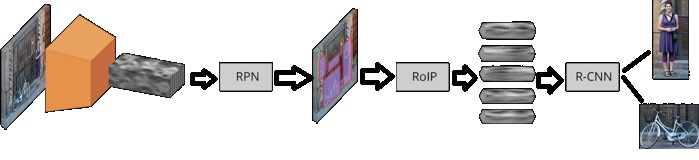
\includegraphics[width=0.8\linewidth]{imagenes/Arquitectura_faster.jpg}
    \caption{Arquitectura de una Faster R-CNN}
    \label{fig:Arquitectura_Faster}
\end{figure}

la figura \ref{fig:Arquitectura_Faster} muestra que la entrada de esta red es una imagen donde se extraen las características por medio de una red neuronal convolucional, para luego usar una Region Proposal Network (RPN), que permite generar varias propuestas de regiones, que se conocen como Bounding Box, estos cuadros delimitadores se reforman utilizando una capa de agrupación de regiones de interés (RoIP), que posteriormente me permite clasificar la imagen dentro de la región propuesta y predecir los valores de desplazamiento con una R-CNN para los cuadros delimitadores, Ren et \textit{al} \cite{Ren_2017}.

Shaoqing et \textit{al} \cite{DBLP:journals/corr/RenHG015} indica que después de extraer las características por medio de una CNN, los pasos que siguen en la Faster R-CNN son:

\begin{itemize}
    \item \textbf{Funcionamiento Region Proposal Network (RPN):} Finalizado el proceso de extracción de características en la última capa de convolución de la CNN, la \textbf{RPN} ejecuta una ventana deslizante sobre el mapa de características, generalmente con dimensiones n x n, generando $n^2$ anclajes/cajas con igual centro ($X_1, Y_1$) pero con \textbf{n} aspectos y \textbf{n} escalas diferentes. 
    
    \begin{figure}[H]
    \centering
    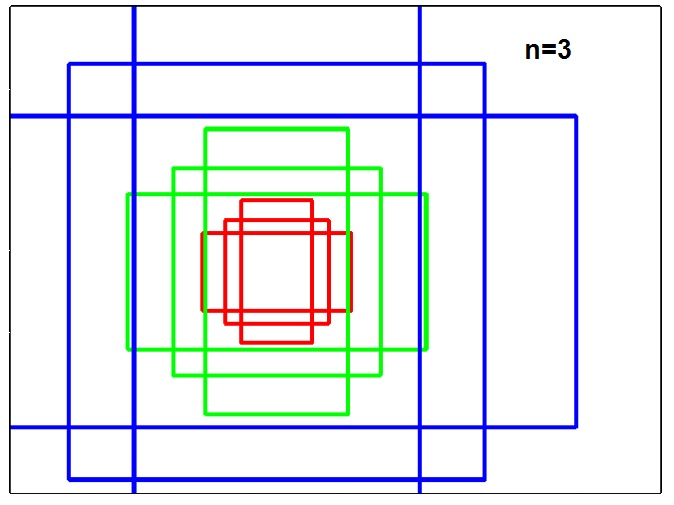
\includegraphics[width=.6\linewidth]{imagenes/anclajes.jpg}
    \caption{Propuestas de anclajes}
    \label{fig:Anclajes}
\end{figure}
    
    Para cada uno de estos anclajes, se calcula un valor p ∗ que indica cuánto se superponen estos anclajes con los cuadros delimitadores(GTBox), así:
    
    IoU = $\frac{A\cap GT}{A \cup GT}$ = $\bigl\{\begin{array}{ccc}
    > 0.7 = Hay & objeto & \\
    < 0.3 = No & hay & objeto
\end{array}$ 
    
IoU = $ \frac{Anclaje \cap GTBox}{Anclaje \cup GTBox}  $
    
    \item \textbf{Funcionamiento de la capa de agrupación de ROI Pooling:} Esta capa recibe muchas propuestas de regiones con tamaños diferentes, extraer características para cada una de esas propuestas  y reduce los mapas de características al mismo tamaño.
    \item \textbf{Funcionamiento Capa final R-CNN:} Después de obtener los mapas de características de \textbf{ROI-P}, estas se usan para la clasificación, a partir de la red neuronal convolucional basada en regiones (R-CNN),intenta imitar las etapas finales de las CNN de clasificación en las que se utiliza una capa completamente conectada para generar una puntuación para cada clase de objeto posible.
\end{itemize}


\subsection{Librerías para Modelos pre-entrenados} 
Existen múltiples librerías de código abierto usadas para \textit{Deep Learning} en lenguaje Python. A continuación, detallamos las usadas en el presente trabajo: 

\Item \textbf{TensorFlow}: Es una interfaz para expresar algoritmos de aprendizaje automático y una implementación para ejecutar dichos algoritmos. Un cálculo expresado con TensorFlow se puede ejecutar con poco o ningún cambio en una amplia variedad de sistemas computacionales heterogéneos, \cite{tensorflow2015-whitepaper}. Su sistema es flexible y se puede utilizar para expresar una amplia variedad de algoritmos, incluidos los algoritmos de entrenamiento e inferencia para modelos de redes neuronales profundas, y se ha utilizado para realizar investigaciones y desplegar sistemas de aprendizaje automático en producción en más de una docena de áreas de ciencias de la computación y otros campos, incluidos el reconocimiento de voz, la visión por computadora, la robótica, la recuperación de información, el procesamiento del lenguaje natural, la extracción de información geográfica y el descubrimiento computacional de drogas. TensorFlow se lanzó como un paquete de código abierto bajo la licencia Apache 2.0 en noviembre de 2015 y están disponibles en www.tensorflow.org. El uso de TensorFlow como una maquina de calculo en paralelo aplicado a problemas de clasificación de imágenes con metodologías de Redes neuronales, es una de las aplicaciones mas recientes de la Inteligencia Artificial.\\

\Item \textbf{OpenCV}\label{opencv}: Es una librería de visión artificial desarrollada por Intel y actualmente publicada bajo licencia BSD, que cuenta con más de medio millar de algoritmos optimizados para realizar las principales tareas de visión artificial, como el procesamiento de imágenes, detección de características o reconocimiento de objetos. La librería cuenta además con diferentes algoritmos de aprendizaje de máquina como máquinas de soporte de vectores (SVM), Naïve Bayes o KNN entre otros, \cite{opencv_library}
Está escrita en C++, es multiplataforma y cuenta con interfaces para trabajar con lenguajes como Java o Python. La gran cantidad de algoritmos disponibles, su velocidad de ejecución y la extensa comunidad de usuarios de que dispone, hacen de OpenCV una herramienta indispensable para desarrollar sistemas de visión artificial basados en software de código abierto.

\subsection{Aplicativos comerciales de reconocimiento de matrículas}

\begin{itemize}
    \item NEC: El analizador de matriculas de vehículos de NEC es uno de los sistemas ANPR, lideres en el mundo. Utiliza algoritmos de alta velocidad y precisión de tipo GLVQ ("\textit{Generalized Learning Vector Quantization}" que en español significa  Cuantización del vector de aprendizaje generalizado).El reconocimiento de matriculas de NEC es altamente preciso incluso en condiciones climáticas adversas. Extrae matriculas vehiculares inclinadas/desplazadas/rotadas Trabaja con imágenes borrosas, con ruido o poco contraste\cite{SoftwareNEC}.
    \item VPAR – Librería de reconocimiento de placas. Neural Labs presenta el software definitivo en el campo del reconocimiento automático de placas de vehículos. Basado en tecnología neuronal propia en constante evolución, proporciona al profesional de la seguridad, un sistema de detección de placas seguro, de fácil instalación e integración en cualquier sistema operativo, y lo que es más importante, con garantía de máxima fiabilidad de lectura\cite{SoftwareVPAR}.
    \item OpenALPR es una biblioteca de reconocimiento automático de matrículas escrita en el lenguaje de programación C++. El software se distribuye en dos versiones: una de código abierto y otra comercial\cite{SoftwareOpen}.
    \item PlateSmart Technologies es una compañía de reconocimiento de matrículas (LPR) basada en software con sede en Oldsmar, Florida. El software independiente de la cámara de la compañía utiliza una cámara de video y una computadora para identificar y grabar placas a través de algoritmos de análisis de video. El producto principal de PlateSmart, ARES, se integra con el hardware existente para crear un sistema LPR\cite{softwarePlateSmart}.
\end{itemize}

\subsection{Bases de datos públicas para el entrenamiento de RNC y Faster R-CNN}

\subsubsection{Ckars74k}\label{Chars74k}

El conjunto de datos \textbf{Chars74k} creado por T. de Campos y M. Varma de Microsoft Research India\cite{de2012chars74k}. Este dataset cuenta con más de 74.000 imágenes de números y letras en formato PNG organizadas en tres colecciones: caracteres manuscritos, caracteres extraídos de fotografías de escenas cotidianas y caracteres generados por ordenador.

Esta última colección cuenta con más de 60.000 imágenes en escala de grises de dígitos y letras representados con diferentes fuentes y estilos (normal, negrita y cursiva), a priori idóneas para que la red CNN “aprenda” a reconocer los patrones de los distintos números y letras de las matrículas\cite{de2009chars74k}. Específicamente incluye:

\begin{itemize}
    \item 64 clases (0-9, AZ, az)
    \item 7705 caracteres obtenidos de imágenes naturales
    \item 3410 personajes dibujados a mano con una tableta
    \item 62992 caracteres sintetizados de fuentes de computadora
\end{itemize}

\subsubsection{Microsoft COCO: \textit{Common Objects in Context}}
\label{sec:coco}
También hay disponibles bases de datos de imágenes para entrenamiento y evaluación de las redes neurales profundas. Los resultados obtenidos en estas evaluaciones se comparan con los de los trabajos originales con la métrica promedio de precisión promedio (mAP). Esta métrica se calcula tomando el promedio sobre mAP calculado en cada umbral de IoU de 0.5 a 0.95, con un paso de 0.05. Las detecciones están limitadas a 100 por imagen. También se hacen algunas consideraciones sobre el tiempo de inferencia de los métodos. Algunas bases de datos son: PASCAL VOC 2007, 2012, MS COCO datasets, Google’s Open Images Dataset V4.

\textit{Common Objects in Context} - COCO, proporciona conjuntos de datos de detección, segmentación y subtitulación de objetos a gran escala \cite{lin2014microsoft}. COCO tiene varias características:

\begin{itemize}
    \item Segmentación de objetos
    \item Reconocimiento en contexto
    \item Segmentación de superpíxeles
    \item 330K imágenes ( > 200K etiquetadas)
    \item 1,5 millones de instancias de objetos
\item 80 categorías de objetos
\item 91 categorías de cosas
\item 5 subtítulos por imagen
\item 250,000 personas con puntos clave
\end{itemize}

El conjunto de datos proporciona múltiples imágenes con las anotaciones correspondientes. Una anotación contiene información sobre el cuadro delimitador y la clasificación de cada objeto en esa imagen que pertenece a una de las clases de interés de ese conjunto de datos. El conjunto de datos puede contener información para otras tareas, como la segmentación\cite{lin2014microsoft}.

\subsection{Segmentación con \textit{Python}}
 El procesamiento de imágenes que ejecuta el módulo \textit{Python} está basado en OpenCV y emplea las siguientes técnicas: 
\begin{itemize}
    \item Conversión a escala de grises: La información de color no es necesaria para el problema planteado y su eliminación facilita la detección de los caracteres de la matrícula. La función  de OpenCV que se utiliza es \textbf{cvtColor}.
    
    \item Thresholding: El thresholding o “técnica del valor umbral” es un método de binarización que permite obtener una imagen en la que quedan claramente definidos los contornos de los caracteres, facilitando el proceso de segmentación o aislamiento de las áreas que los contienen. La función  de OpenCV que se utiliza es \textbf{thresholding}.
    
    \item Desenfoque Gaussiano: Aplicar efecto de suavizado en la imagen para eliminar el ruido. En concreto, se aplica un filtro de desenfoque Gaussiano que consiste en mezclar ligeramente los niveles de gris entre píxeles adyacentes, lo que da como resultado una imagen con los bordes más suaves en la que se pierden pequeños detalles, de manera similar a lo que ocurre en las fotografías desenfocadas. La función  de OpenCV que se utiliza es \textbf{GaussianBlur}.
    
    \item Detección de contornos: Los contornos o bordes son curvas que unen conjuntos de píxeles contiguos que tienen el mismo color o intensidad. Estas curvas permiten localizar las fronteras de los objetos de la imagen, y su detección es fundamental para que un sistema de visión artificial pueda reconocer o detectar formas en una imagen. Las funciones  de OpenCV que se utilizan son \textbf{findContours} y \textbf{boundingRect}.
\end{itemize}.

%----------------------

%-=============================================
\chapter{Metodología de la investigación}
%==============================================
%-------------------------------
\section{Diseño Metodológico}
%------------------------------
Hemos construido un sistema de reconocimiento de placas vehiculares, haciendo uso de redes neuronales convolucionales. El sistema fue creado realizando cambios en los parámetros de una RNC y, en cada cambio, ensayos de entrenamiento para observar el rendimiento; y así escoger la arquitectura que dio los mejores resultados. Por tal motivo, hemos considerado que se trata de una investigación de tipo experimental. 

El objetivo es diseñar un sistema experto que permita reconocer en una imagen de una placa colombiana, los 6 caracteres que ésta contiene. Con el fin de lograr este objetivo y responder cada una de las preguntas de investigación, hemos realizado el siguiente procedimiento:

\begin{itemize}

\item[i.] Estudio de todo lo relacionado con las RNC: Conocer su historia; los campos de aplicación; las diferentes arquitecturas y su estructura interna; los requerimientos de la base de datos para su entrenamiento; las herramientas computacionales para su implementación; las formas de medir su rendimiento; entre otros (ver sección \ref{marcoteorico}). Esta etapa nos motivó inicialmente a construir desde cero nuestra propia RNC; y luego, a usar la técnica de detección de objetos. 
    
\item[ii.] Construcción de una base de datos a partir de imágenes segmentadas de caracteres de placas colombianas. Tal base de datos la hemos llamado \textit{CharsPlateCol}. 
    
\item[iii.] Construcción de una RNC desde cero para ser entrenada con la base de datos construida \textit{CharsPlateCol}.
    
\item[iv.] Construcción de una base de datos de caracteres similares a los caracteres que se presentan en placas colombianas a partir de depuración de la base de datos pública \textit{Chars74k}. Tal base de datos la hemos llamado \textit{Chars34k}. 
    
\item[v.] Entrenamiento de la RNC construida desde cero, usando la base de datos \textit{CharsPlateCol} construida inicialmente, más la base de datos \textit{Chars34k}.
    
\item[vi.] Construcción de una base de datos usando cuadros delimitadores (Bonding Boxing) en imagenes de placas colombianas. Tal base de datos la hemos llamado \textit{CharsBoxPlateCol}.
 
 \item[vii.] Implementación de transferencia de aprendizaje para el entrenamiento de una Faster R-CNN usando la base de datos \textit{CharsBoxPlateCol} .
    \end{itemize}
%__________________________
%    \item Estudio del procesamiento de imágenes con la librería \textit{OpenCv} (ver sección  \ref{opencv}).

 %   \item Construcción de un código en \textit{Python} usando librería de \textit{OpenCv}, para realizar la segmentación de la placa y sus 6 caracteres. Estas imágenes  la entrada de nuestra RNC entrenada previamente.
    
  %  \item Construir una base de datos con imágenes de 40 x 80 píxeles con alta variabilidad en cada una de las 36 clases, obtenidas inicialmente de placas colombianas reales, luego realizamos el entrenamiento de la RCN con esta data.
    
    
 %   \item A nuestro dataset de placas colombianas construido anteriormente, le anexamos imágenes a cada una de las 36 clases de la data publica Chars74k, para explorar si se mejora el rendimiento de la Red neuronal convolucional.
    
  %  \item Construir un dataset para el entrenamiento de una Faster R-CNN.
    
  %  \item Entrenar una Faster R-CNN con nuestra data y por medio de la inferencia, que es el uso de redes pre-entrenadas
   
 %   \item Calcular todas las métricas de rendimiento de nuestra red neuronal y de la Faster R-CNN, para así responder las preguntas de investigación. 

%------------------------------------
\section{Datos y técnicas de recolección}
%--------------------------------------
La eficacia de un sistema de clasificación de imágenes basado en una red neuronal convolucional depende tanto de la arquitectura y ajustes de la red, como del conjunto de datos empleado para su entrenamiento. Este último debe ser suficientemente amplio y representativo del problema que se quiere resolver.

Nuestro objetivo es diseñar un sistema de visión artificial para el reconocimiento de placas de automóviles colombianos a partir de la imagen de la parte frontal del vehículo, de tal forma que se pudiesen distinguir, por un ojo humano normal, su placa; aunque no necesariamente todos los 6 caracteres que la componen. Este sistema puede ser implementado para el control de acceso a vehículos, en lugares tales como  parqueaderos.

En nuestro caso, para tener una base de datos adecuada a la aplicación que se quiere implementar, inicialmente hemos usado imágenes de vehículos tomadas por cámaras instaladas en parqueaderos de centros comerciales en Colombia. Estás imágenes fueros tomadas en condiciones ambientales reales. Esta base de datos la hemos llamado \textit{CharsPlateCol} y garantiza en cierta medida la variabilidad en condiciones ambientales que se exige en el entrenamiento de una RNC. Luego, para ampliar la base de datos construida, hemos escogido caracteres de la base de datos pública \textit{Chars74k}. Esta base de datos la hemos llamado \textit{Chars34k}. Finalmente, hemos construido una base de datos llamada \textit{CharsBoxPlateCol}. Esta base de datos fue especialmente construida para aplicar la técnica de detección de objetos; en este caso, los objetos a detectar son los caracteres de las placas.  
A continuación describiremos las bases de datos construidas:

%En primera instancia analizaremos la construcción de la data de caracteres segmentados y luego la data chars74K, debemos tener presente que este conjunto de datos está formado por 36 clases, que representa 10 dígitos y 26 letras que son las usadas en el formato de 3 letras y 3 números en las placas colombianas. 


\subsection{Base de datos \textit{CharsPlateCol}} \label{CharsPlateCol2.5k}

Esta base de datos de imágenes de caracteres de placas colombianas, ha sido construida a partir de imágenes capturadas con una cámara instalada en un parqueadero tal como se muestra en la figura \ref{fig:imagen completa}. 

\begin{figure}[H]
\centering
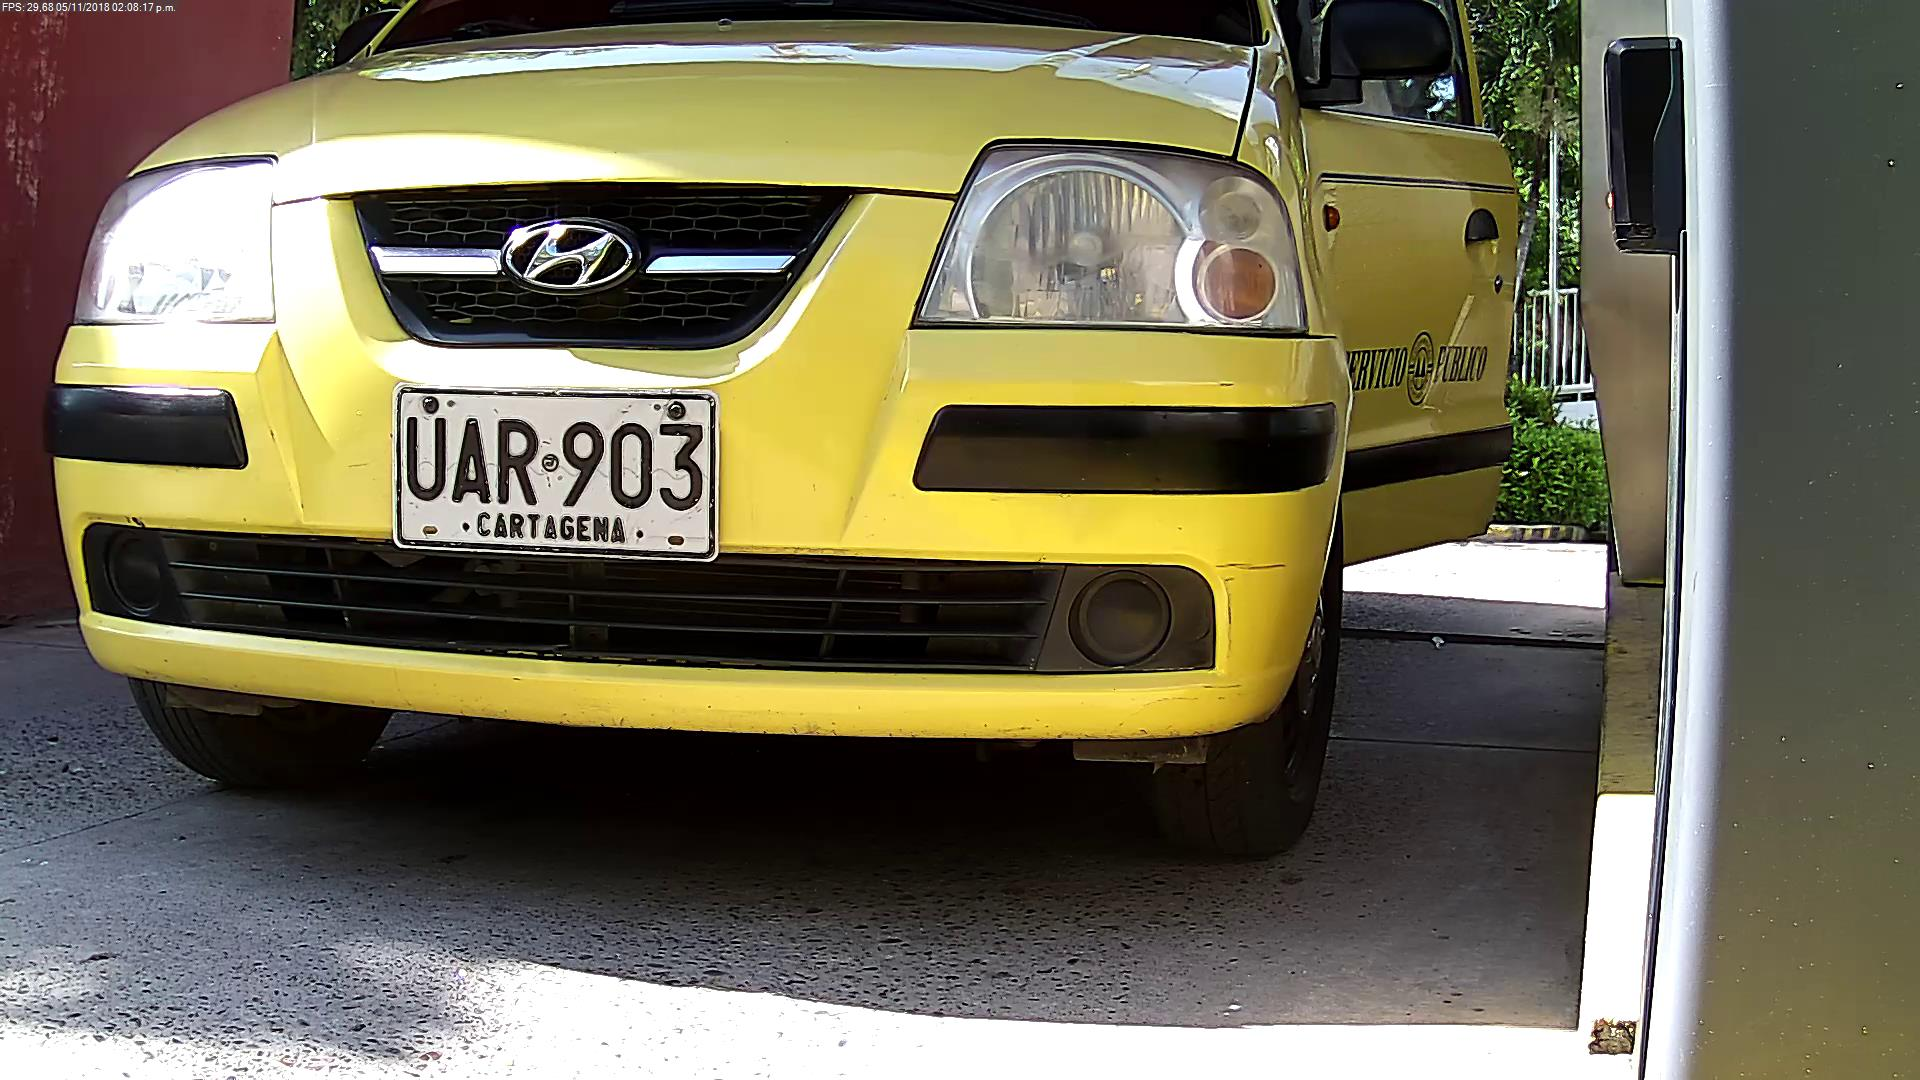
\includegraphics[width=0.7\linewidth]{imagenes/MODELO_4/segmentacion/carro4.jpg} 
\caption{ Cargamos Imagen}
\label{fig:imagen completa}
\end{figure}

La extracción de los caracteres se realizó con la librería OpenCV para el tratamiento de imágenes (ver sección \ref{opencv}). Seguidamente se explicará el proceso realizado, tomando como ejemplo la imagen del automovil mostrado en la figura \ref{fig:imagen completa}:    

 \begin{enumerate}
     \item  Se recorta la imagen para disminuir la región donde se encuentra la placa y facilitar el proceso de extracción. El resultado se muestra en la figura(\ref{fig:recorter}).
     
    \begin{figure}[H]
    \centering
    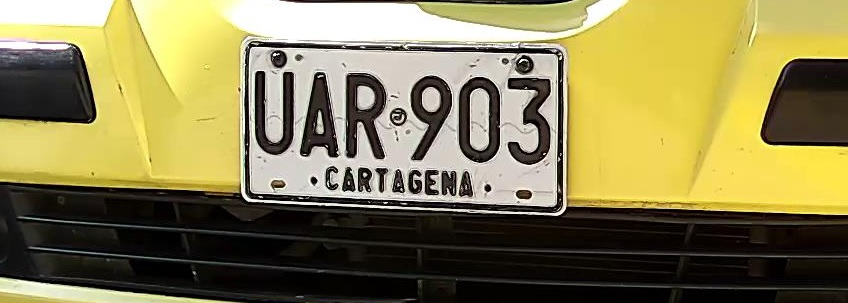
\includegraphics[width=0.5 \linewidth]{imagenes/MODELO_4/segmentacion/recorte.jpg} 
    \caption{ Recorte de la imagen}
    \label{fig:recorter}
    \end{figure}
     
     \item Se convierte a escala de grises. El resultado se muestra en la figura \ref{fig:Escala de grises}.
     
     \begin{figure}[H]
    \centering
    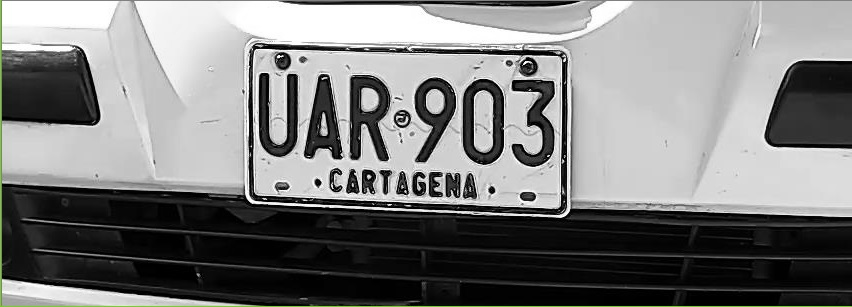
\includegraphics[width=0.5 \linewidth]{imagenes/MODELO_4/segmentacion/gris.jpg} 
    \caption{ Escala de grises}
    \label{fig:Escala de grises}
    \end{figure}
    
     \item Se convierte a una imagen a binaria (solamente ceros y unos). El resultado se observa en la figura \ref{fig:Convertimos la imagen a binaria}
     
     \begin{figure}[H]
    \centering
    
\includegraphics[width=0.5 \linewidth]{imagenes/MODELO_4/segmentacion/umbral.jpg} \caption{Convertimos la imagen a binaria}
    \label{fig:Convertimos la imagen a binaria}
    \end{figure}
     
     \item  se realiza un desenfoque Gaussiano para ampliar la frontera de los bordes. El resultado se aprecia en la figura \ref{fig:Desenfoque Gaussiano}.
     
     \begin{figure}[H]
    \centering
    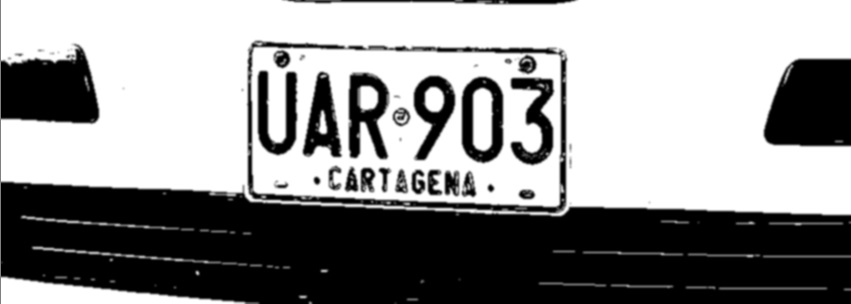
\includegraphics[width=0.5 \linewidth]{imagenes/MODELO_4/segmentacion/suavi.jpg} 
    \caption{Desenfoque Gaussiano}
    \label{fig:Desenfoque Gaussiano}
    \end{figure}
     
     \item Se resaltan los bordes con un filtro Canny. El resultado se puede ver en la figura \ref{fig:Bordes con Canny}.
     
     \begin{figure}[H]
    \centering
    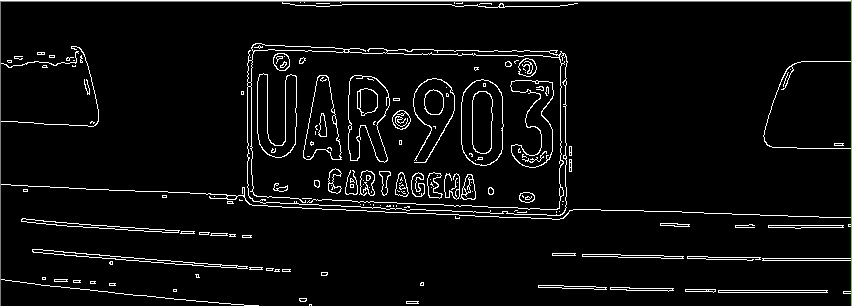
\includegraphics[width=0.5 \linewidth]{imagenes/MODELO_4/segmentacion/borde.jpg} 
    \caption{Bordes con Canny}
    \label{fig:Bordes con Canny}
    \end{figure}
    
     \item Se identifica la región de interés. El resultado se ve en la figura \ref{fig:Region ROI}, donde las lineas verdes son todos los contornos identificados y el cuadro  azul es la zona de interés (la placa).
     
     \begin{figure}[H]
    \centering
    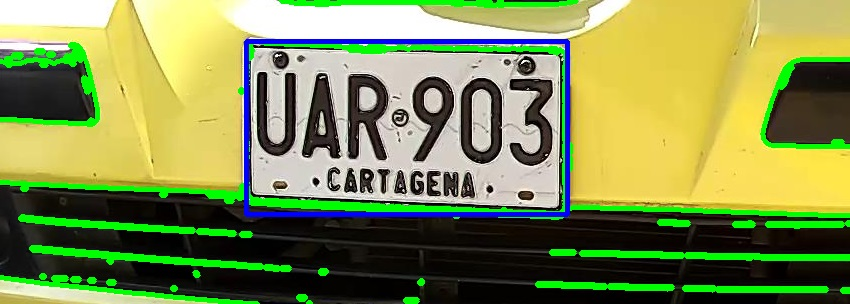
\includegraphics[width=0.5 \linewidth]{imagenes/MODELO_4/segmentacion/roi.jpg}
    \caption{Región de interés}
    \label{fig:Region ROI}
    \end{figure}

    
    \item Se recorta la región de interés. El resultado se observa en la figura \ref{fig:Extracción placa}.
     
     \begin{figure}[H]
    \centering
    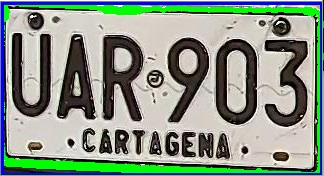
\includegraphics[width=0.5 \linewidth]{imagenes/MODELO_4/segmentacion/placa.jpg} 
    \caption{Extracción placa}
    \label{fig:Extracción placa}
    \end{figure}
     
     \item Finalmente de la placa segmentada se recortan los caracteres. El resulyado se puede observar en la figura \ref{fig:segmentación de caracteres}. Son estos caracteres los que hacen parte de la base de datos construida.

    \begin{figure}[H]
    \centering
    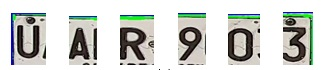
\includegraphics[width=0.6 \linewidth]{imagenes/MODELO_4/segmentacion/segmentacion_figura2.jpg} \caption{segmentación de caracteres}
    \label{fig:segmentación de caracteres}
    \end{figure}
     
 \end{enumerate}
 
 %     \begin{figure}[H]
  %  \centering
   % 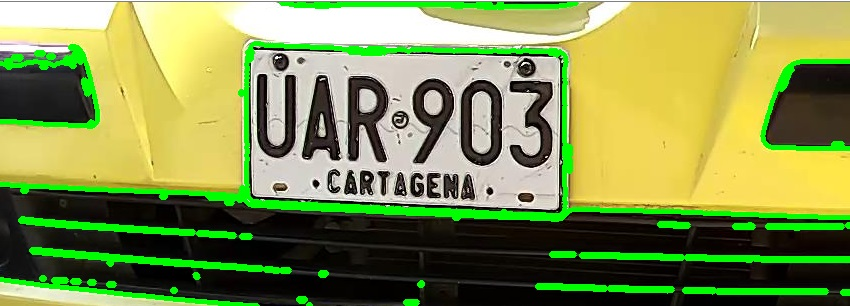
\includegraphics[width=0.5 \linewidth]{imagenes/MODELO_4/segmentacion/contor.jpg} 
    %\caption{Identificar y dibujar contornos}
    %\label{fig:Identificar y dibujar contornos}
    %\end{figure}


%\end{enumerate}


%La red neuronal convolucional que será entrenada con esta base de datos, tiene que clasificar los 6 caracteres de placas colombianas diseñadas con 3 letras y 3 números. Por tal motivo, hicimos el proceso descrito anteriormente con placas reales que se lograron segmentar. 

En total se segmentaron 432 placas. La figura \ref{fig:Muestra de placas segmentadas} es una muestra de las placas colombianas una vez segmentadas y que fueron usadas para obtener cada uno de los caracteres de la base de datos \textit{CharsPlateCol2.5k}

\begin{figure}[H]
  {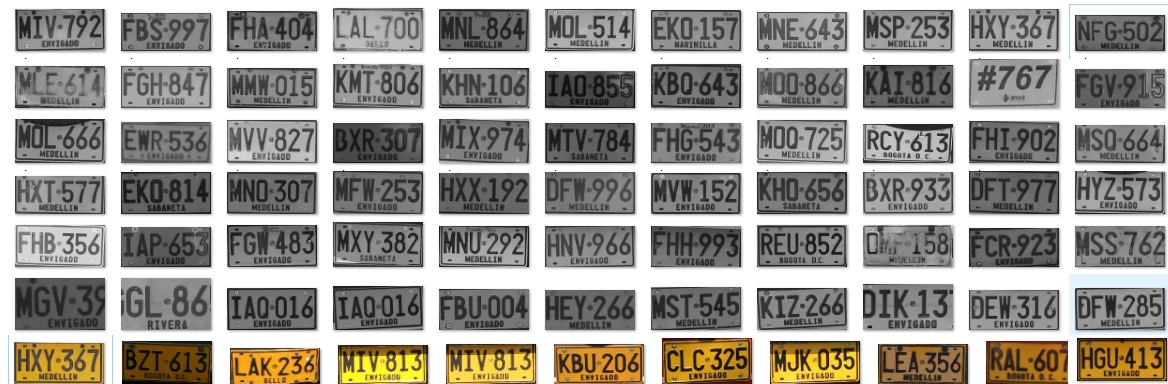
\includegraphics[width=1\linewidth]{imagenes/RESULTADOS/PLACAS_PA_SEGMENTAR.jpg}}
   \caption{Muestra de placas segmentadas}
    \label{fig:Muestra de placas segmentadas}  
\end{figure}

%Con las placas segmentadas, la siguiente etapa es el proceso de segmentación que se realizó inicialmente de forma manual. Luego, se diseñó un código para la segmentación automática de los 6 caracteres por placa, 

La base de datos \textit{CharsPlateCol2.5k} así construida, tiene un total de 2593 imágenes de caracteres (letras y números) con un tamaño de 40 x 80 píxeles con 3 canales. En la figura \ref{fig:Muestra caracter D base de datos} se puede observar una muestra de letras D pertenecientes a la base de datos construida.

\begin{figure}[H]
  {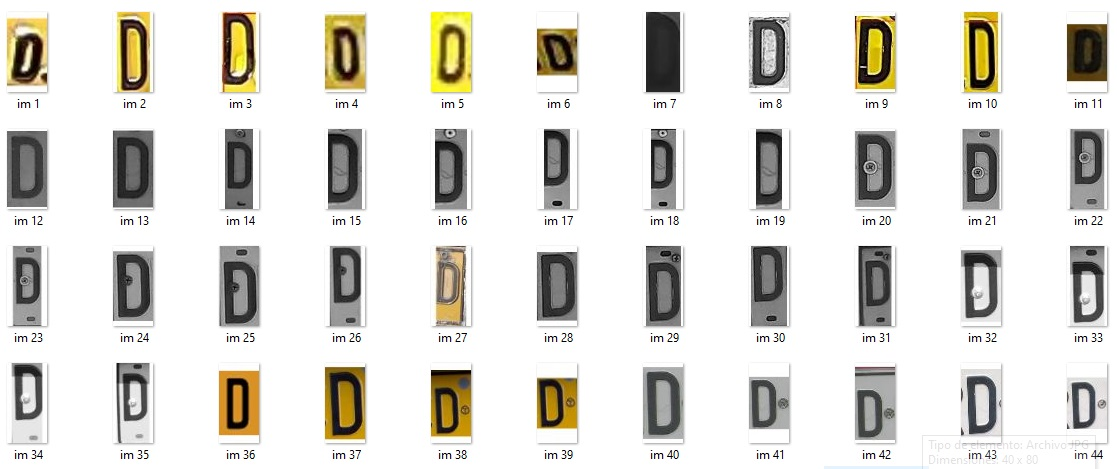
\includegraphics[width=1\linewidth]{imagenes/RESULTADOS/muestra_letra.jpg}}
   \caption{Muestra caracter D base de datos segmentadas \textit{CharsPlateCol}}
    \label{fig:Muestra caracter D base de datos}
\end{figure} 

En la base de datos se distinguen 36 clases: 10 números del 0 al 9 y 26 letras del alfabeto español. En el cuadro \ref{table:Caracteres por clase} se muestra la cantidad de imágenes que tenemos en cada clase y en la figura \ref{fig:frecuencia} un diagrama de frecuencias. 

\begin{table}[H]
\begin{center}
\resizebox{0.5\textwidth}{!}{
\begin{tabular}{||c|c|
|c|c||}
\hline
 Clase & Frecuencia & Clase & Frecuencia\\
\hline \hline
000 & 106 & letra I & 106\\\hline
001 & 55 & letra J & 60\\\hline
002 & 62 & \textcolor{red}{letra K} & \textcolor{red}{50}\\\hline
\textcolor{green}{003} & \textcolor{green}{111} & letra L & 54\\\hline
004 & 61 & letra M & 62\\\hline
005 & 62 & letra N & 94\\\hline
006 & 72 & letra O & 99\\\hline
\textcolor{red}{007}&\textcolor{red}{ 50} & letra P & 51\\\hline
008 & 56 & letra Q & 57\\\hline
009 & 52 & letra R & 70\\\hline
letra A & 59 & letra S & 101\\\hline
\textcolor{red}{letra B} & \textcolor{red}{50} & letra T & 54\\\hline
\textcolor{green}{letra C} & \textcolor{green}{120} & letra U & 112\\\hline
letra D & 89 & letra V & 54\\\hline
letra E & 55 & letra W & 54\\\hline
letra F & 51 & letra X & 105\\\hline
letra G & 62 & letra Y & 115\\\hline
letra H & 58 & letra Z & 63\\ \hline
\hline
Total imágenes & \multicolumn{3}{|c||}{2593}\\
\hline \hline
\end{tabular}
}
\caption{\label{table:Caracteres por clase}Cantidad de imágenes por clase en la base de datos \textit{CharsPlateCol}}
\end{center}
\end{table}

\begin{figure}[H]
\centering
  {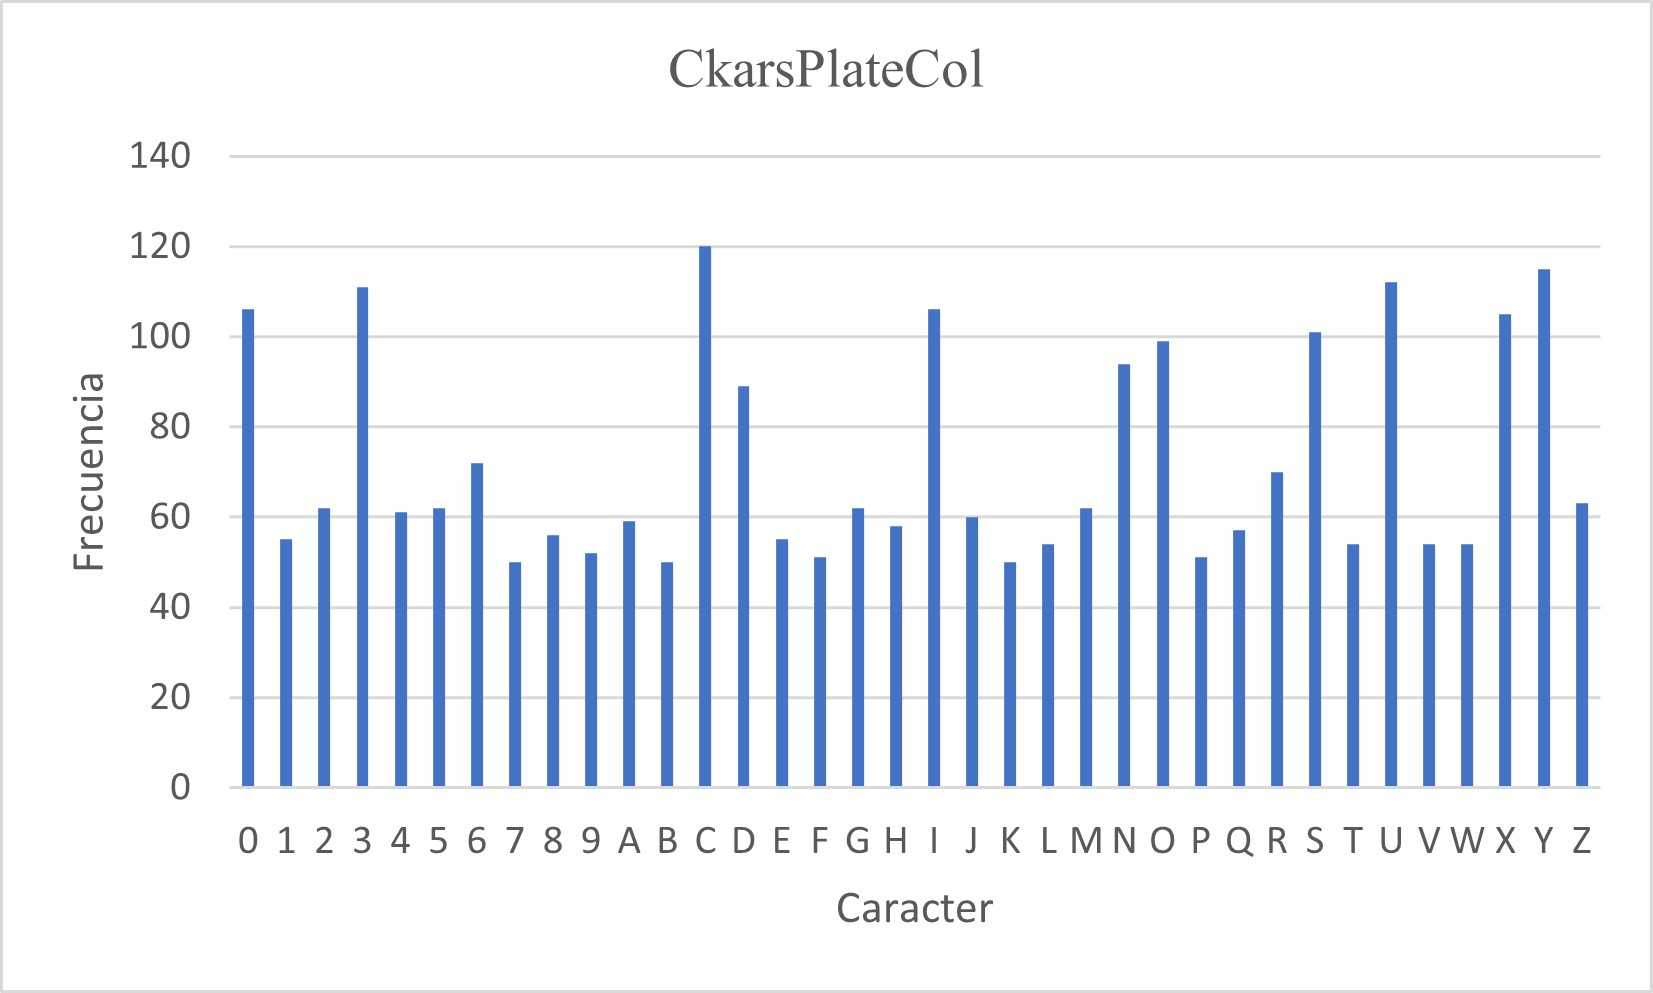
\includegraphics[width=0.8\linewidth]{imagenes/frecuenciaCaracter1.jpg}}
   \caption{Frecuencia de cada caracter en la base de datos \textit{CharsPlateCol}}
    \label{fig:frecuencia}
\end{figure} 

Se puede observar que la distribución de la cantidad de imágenes por cada carácter no es la misma, ya que en las 432 placas, no se encontraban la misma cantidad de caracteres. Lo que indica, que nuestra base de datos es heterogénea con relación al número imágenes por caracter. Esta heterogeneidad puede deberse a que las imágenes fueron tomadas en una misma ciudad y tienden a repetirse unos caracteres más que otros.  

%Con las 36 clases definidas, que representa cada uno de los caracteres, realizamos el conteo de los caracteres por clase, y encontramos que prevalecen las imágenes de la letra \textbf{C} con 120 de ellas y el número \textbf{3} con 111, debemos resaltar que tenemos caracteres con solo 50 imágenes, fue así, y logramos crear una data con un total de 2593 imágenes. 


\subsection{Base de datos \textit{Chars34k}} \label{Chars34k}

Como no se tenía una base de datos de diferentes ciudades colombianas para tener una base de datos un poco más homogénea, se decidió completarla con caracteres de la base de datos pública \textit{Chars74k} (ver sección \ref{Chars74k}). Este dataset cuenta con 74.000 imágenes de números y letras con mucha variabilidad y estilos. En la figura \ref{fig:Muestra de dataset chars74K} se observa una muestra de caracteres de tal base de datos. En este conjunto no todos los caracteres son similares a los usados en las placas colombianas, por ejemplo la base de datos tiene caracteres en minúsculas y las placas colombianas solamente usan caracteres en mayúsculas. Es así, que se hizo necesario realizar una depuración para escoger finalmente, un conjunto de aproximadamente 34 mil imágenes de caracteres (números y letras)  similares a los usados en las placas colombianas. Por tal razón, hemos llamado está base de datos \textit{Chars34k}.     
%-------------------------
%entrenar la red neuronal del sistema propuesto se ha elegido el conjunto de  datos \textit{Chars74k} (ver sección \ref{Chars74k}), Este dataset cuenta con más de 74.000 imágenes de números y letras, con mucha variabilidad, lo implica realizar necesariamente una depuración, para así escoger aquellas imágenes similares a los caracteres usados en placas Colombianas.

\begin{figure}[H]
\begin{center}
   {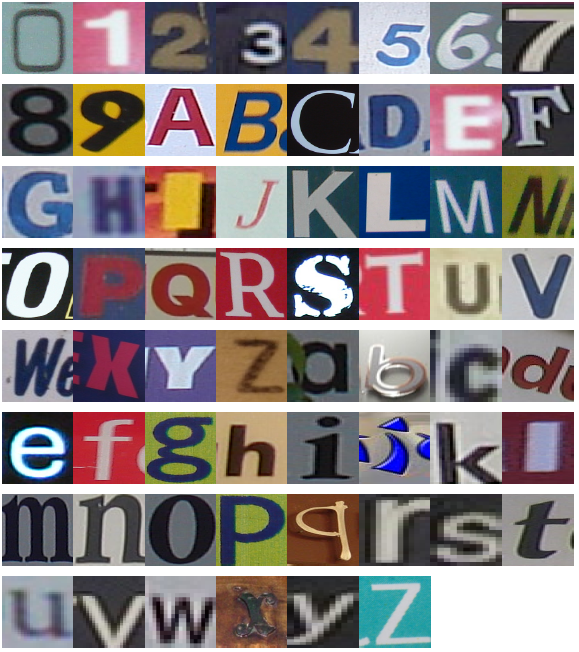
\includegraphics[width=.37\linewidth]{charks74.png}}
    \caption{Muestra de dataset chars74K}
    \label{fig:Muestra de dataset chars74K} 
\end{center}
\end{figure}

 %Esta depuración inicialmente fue solo de las letras minúsculas, puesto que las placas colombianas solo usan letras mayúsculas y dígitos, así que se revisamos más de 60 carpetas y se logró obtener 41772 archivos, distribuidos en 36 directorios, que representan 26 letras y 10 números.

%Se hizo este proceso de depuración en varias ocasiones, hasta obtener los caracteres semejantes a los usados en las placas colombianas.

\subsection{Base de datos conformada por \textit{Chars34k} y \textit{CharsPlateCol}} \label{Chars34k}

Para tener una base de datos mejor balanceada y representativa, se unieron las bases de datos \textit{CharsPlateCol2.5k} y \textit{Chars34k}. En la figura \ref{fig:Muestra de dataset chars34K} se puede observar una muestra con imágenes de la letra G tanto de placas colombianas como de la base de datos \textit{Chars34k}. 
%tomaron cerca de 1000 placas colombianas y se segmentaron sus caracteres con el objetivo de balancear la data a usar en el entrenamiento de la Red neuronal convolucional, con 37.398 imágenes de 40 x 80 píxeles distribuidas en 36 carpetas. La figura \ref{fig:Muestra de dataset chars34K} es la muestra de la letra G en la base de datos \textit{chars34K}, que incluye letras de placas colombianas y letras depuradas de la base de datos \textit{chars74K}.
\begin{figure}[H]
\begin{center}
   \subfigure[]{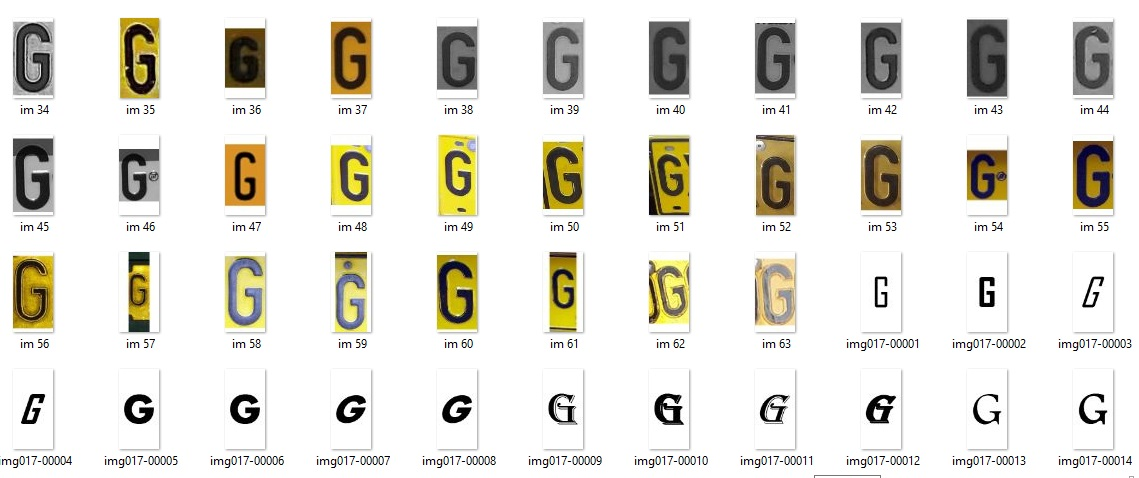
\includegraphics[width=.9\linewidth]{muestra_data.jpg}}
    \caption{Una muestra de imagenes de la letra G tanto en \textit{Chars34k} y \textit{CharsPlateCol}}
    \label{fig:Muestra de dataset chars34K} 
\end{center}
\end{figure}

En el cuadro \ref{table:Caracteres por clase} se muestra la cantidad de imágenes en cada clase y en la figura \ref{fig:frecuencia2} un diagrama de frecuencias. El conjunto total contiene 37.398 imágenes con tamaño de 40x80 píxeles. Se puede observar en el diagrama que se obtiene una base de datos mejor balanceada, salvo el número 8 que tiene menos frecuencia.

%Luego de la construcción de la data \textit{chars34K}, contabilizamos el número de caracteres por clase, y encontramos que prevalecen las imágenes de la letra \textbf{X} con 2065 de ellas y el número \textbf{3} con 1162

\begin{table}[H]
\begin{center}
\resizebox{0.5\textwidth}{!}{
\begin{tabular}{||c|c||c|c||}
\hline \hline
 Clase & Frecuencia & Clase & Frecuencia\\
\hline\hline
000  &  1134 & letra I  &  1118\\\hline
001  &  1035 & letra J  &  1035\\\hline
002  &  1018 & letra K & 997\\\hline
\textcolor{green}{003}  & \textcolor{green}{ 1162} & letra L & 949\\\hline
004 &  1026 & letra M  &  1012\\\hline
005 & 971 & letra N  &  1075\\\hline
006 & 993 & letra O  &  1105\\\hline
007  &  1018 & letra P  &  1002\\\hline
\textcolor{red}{008} & \textcolor{red}{86} & \textcolor{red}{letra Q} &\textcolor{red}{ 886}\\\hline
009 & 995 & letra R & 999\\\hline
letra A  &  1025 & letra S  &  1102\\\hline
letra B  &  1016 & letra T  &  1001\\\hline
letra C  &  1173 & letra V & 994\\\hline
letra D  &  1117 & letra U  &  1121\\\hline
letra E  &  1023 & letra W  &  1005\\\hline
letra F & 991 & \textcolor{green}{letra X} & \textcolor{green}{2065}\\\hline
letra G  &  1036 & letra Y  &  1104\\\hline
letra H & 986 & letra Z  &  1022\\
\hline \hline
Total imágenes & \multicolumn{3}{|c|}{37397} \\
\hline \hline
\end{tabular}
}
\caption{\label{table:imagenes por clase chars74k}Cantidad de imágenes por clase en la base de datos obtenida al unir \textit{Chars74k} con \textit{CharsPlateCol}}
\end{center}
\end{table}

\begin{figure}[H]
\centering
  {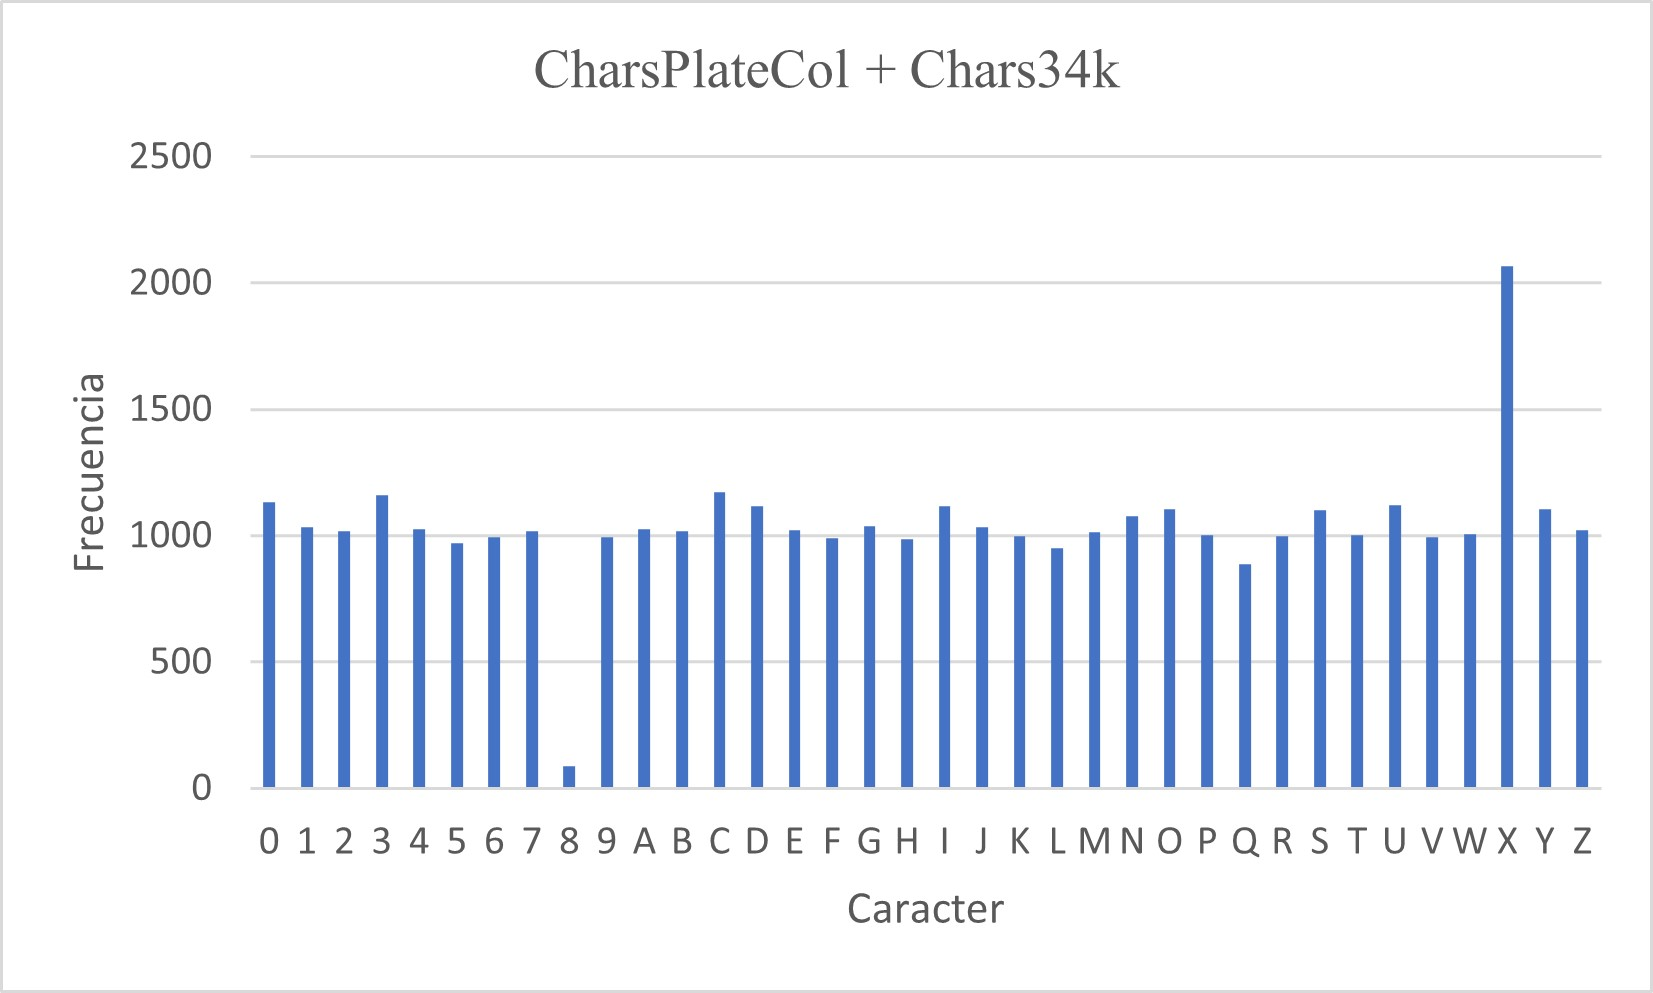
\includegraphics[width=0.8\linewidth]{imagenes/frecuenciaCaracter2.jpg}}
   \caption{Frecuencia de cada caracter en la base de datos resultante de unir \textit{Chars34k} con \textit{CharsPlateCol}}.
    \label{fig:frecuencia2}
\end{figure}

%-----------------------------------------------------
\subsection{Base de datos \textit{CharsBoxPlateCol}} \label{sec:basedatos3}
%----------------------------------------------------
Esta base de datos se ha construido para realizar transferencia de aprendizaje usando el modelo Faster R-CNN Inception v2 (COCO) de TensorFlow. Este modelo utiliza la técnica de detección de objetos (ver sección \ref{sec:deteccionobjetos}). La base de datos para el entrenamiento de este tipo de modelos debe incluir, además de la imagen de la placa, las coordenadas del rectángulo donde esta inscrito cada caracter a ser detectado. 
El proceso para obtener las coordenadas del objeto, en este caso de cada caracter, dentro de la imagen, se denomina Etiquetado (Labeling). Nosotros hemos realizado el proceso de etiquetado usando la aplicación \textbf{LabelImg}. Esta aplicación tiene una interfaz que permite al usuario delimitar con un rectángulo (Bonding box) cada uno de los caracteres dentro de la imagen y realizar el etiquetado con la clase correspondiente. La figura \ref{fig:etiquetas deteccion} muestra un ejemplo del funcionamiento de la interfaz. El usuario va colocando los rectángulos delimitadores sobre los caracteres B,X,U,3,0 y 4; en un submenú a la derecha  va escogiendo la etiqueta correspondiente a cada caracter dentro del rectángulo.   

\begin{figure}[H]
\centering
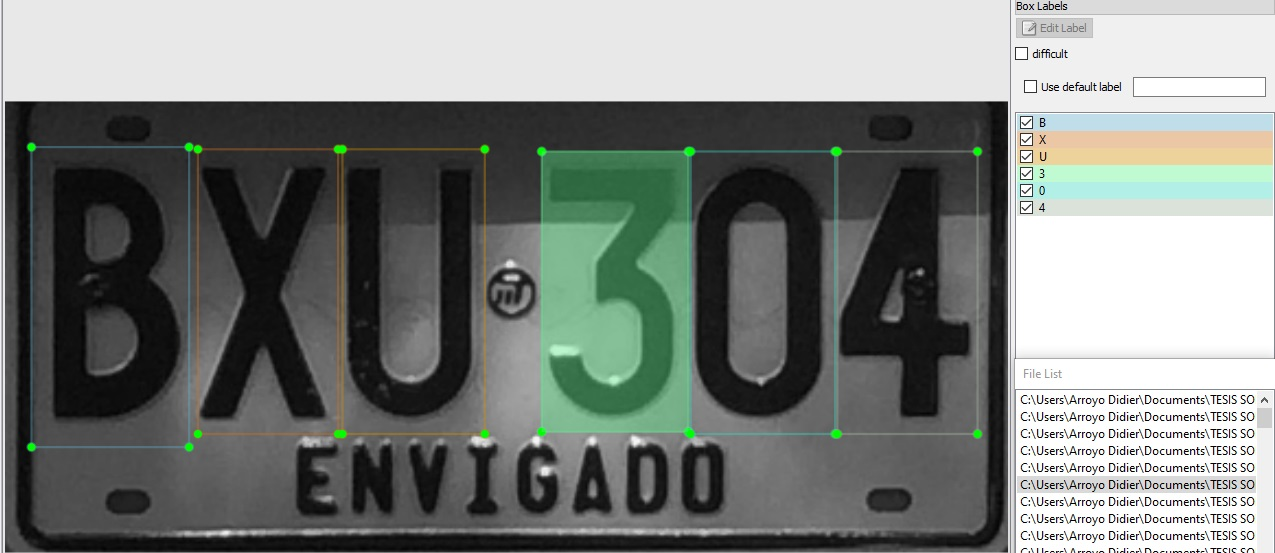
\includegraphics[width=0.5\textwidth]{imagenes/MODELO_5/ETIQUETA_MOD_IV.jpg} \caption{Aplicación LabelImg. Ejemplo de su interfaz de usuario para la obtención de las coordenadas del rectangulo delimitador}
\label{fig:etiquetas deteccion}
\end{figure}
 La aplicación genera un archivo en formato \textbf{Xml} con las coordenadas de cada uno de los rectangulos para cada clase (caracter) dentro de la imagen de la placa.  
 
\begin{figure}[H]
\centering
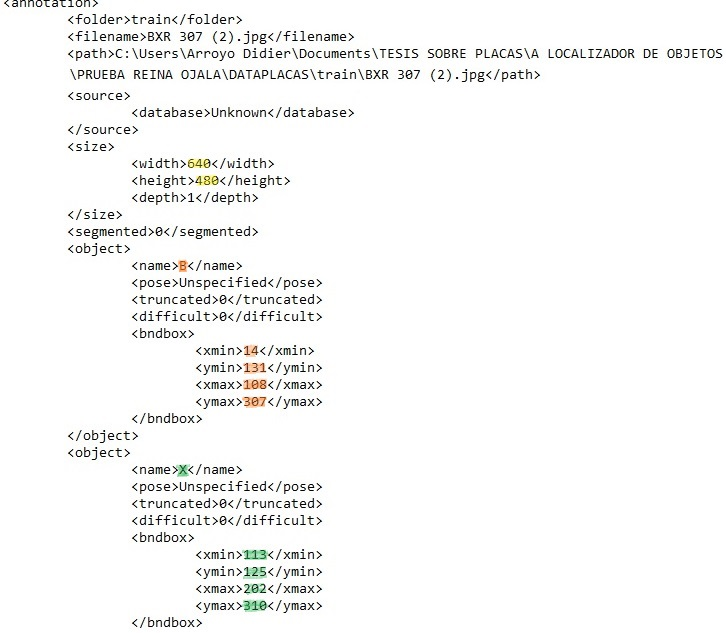
\includegraphics[width=0.7\linewidth]{imagenes/RESULTADOS/annonations.jpg} \caption{Archivo Xml generado por LabelIng para la placa en la Figura \ref{fig:etiquetas deteccion}.}
\label{fig:Ejemplo anotación Xml}
\end{figure}
 
 
 La Figura \ref{fig:Ejemplo anotación Xml} muestra una parte del contenido del archivo generado para el ejemplo considerado. Allí podemos ver (resaltados con colores) el tamaño de la placa y las coordenadas de las letras B y X.
Para nuestra base de datos se escogieron 177 placas, resultando en total 888 caracteres etiquetados. En la tabla \ref{table:frecuencia3} se muestra la cantidad de imágenes en cada clase y en la figura \ref{fig:frecuencia3} un diagrama de frecuencias. Se puede observar en el diagrama que se obtiene una base de datos muy desbalanceada.

\begin{table}[H]
\begin{center}
\resizebox{0.5\textwidth}{!}{
\begin{tabular}{||c|c||c|c||}
\hline \hline
 Clase & Frecuencia & Clase & Frecuencia\\
\hline\hline
000  &  36 & letra I  &  20\\\hline
001  &  27 & letra J  &  3\\\hline
002  &  39 & letra K & 28\\\hline
003  & 53 & letra L & 21\\\hline
004 &  47 & letra M  &  52\\\hline
005 & 53 & letra N  &  15\\\hline
006 & 55 & letra O  &  21\\\hline
007  &  41 & letra P  &  6\\\hline
008 & 28 & letra Q & 13\\ \hline
009 & 33 & letra R & 14\\\hline
letra A  &  18 & letra S  &  11\\\hline
letra B  &  19 & letra T  &  13\\\hline
letra C  &  3 & letra u & 12\\\hline
letra D  &  15 & letra v  &  21\\\hline
letra E  &  18 & letra W  &  16\\\hline
letra F & 47 & letra X & 21 \\\hline
letra G  &  16 & letra Y  &  9\\\hline
letra H & 39 & letra Z  &  5\\
\hline \hline
Total etiquetas & \multicolumn{3}{|c|}{888} \\
\hline \hline
\end{tabular}
}
\caption{\label{table:frecuencia3}Cantidad de etiquetas por clase en la base de datos\textit{CharsBoxPlateCol}}
\end{center}
\end{table}

\begin{figure}[H]
\centering
  {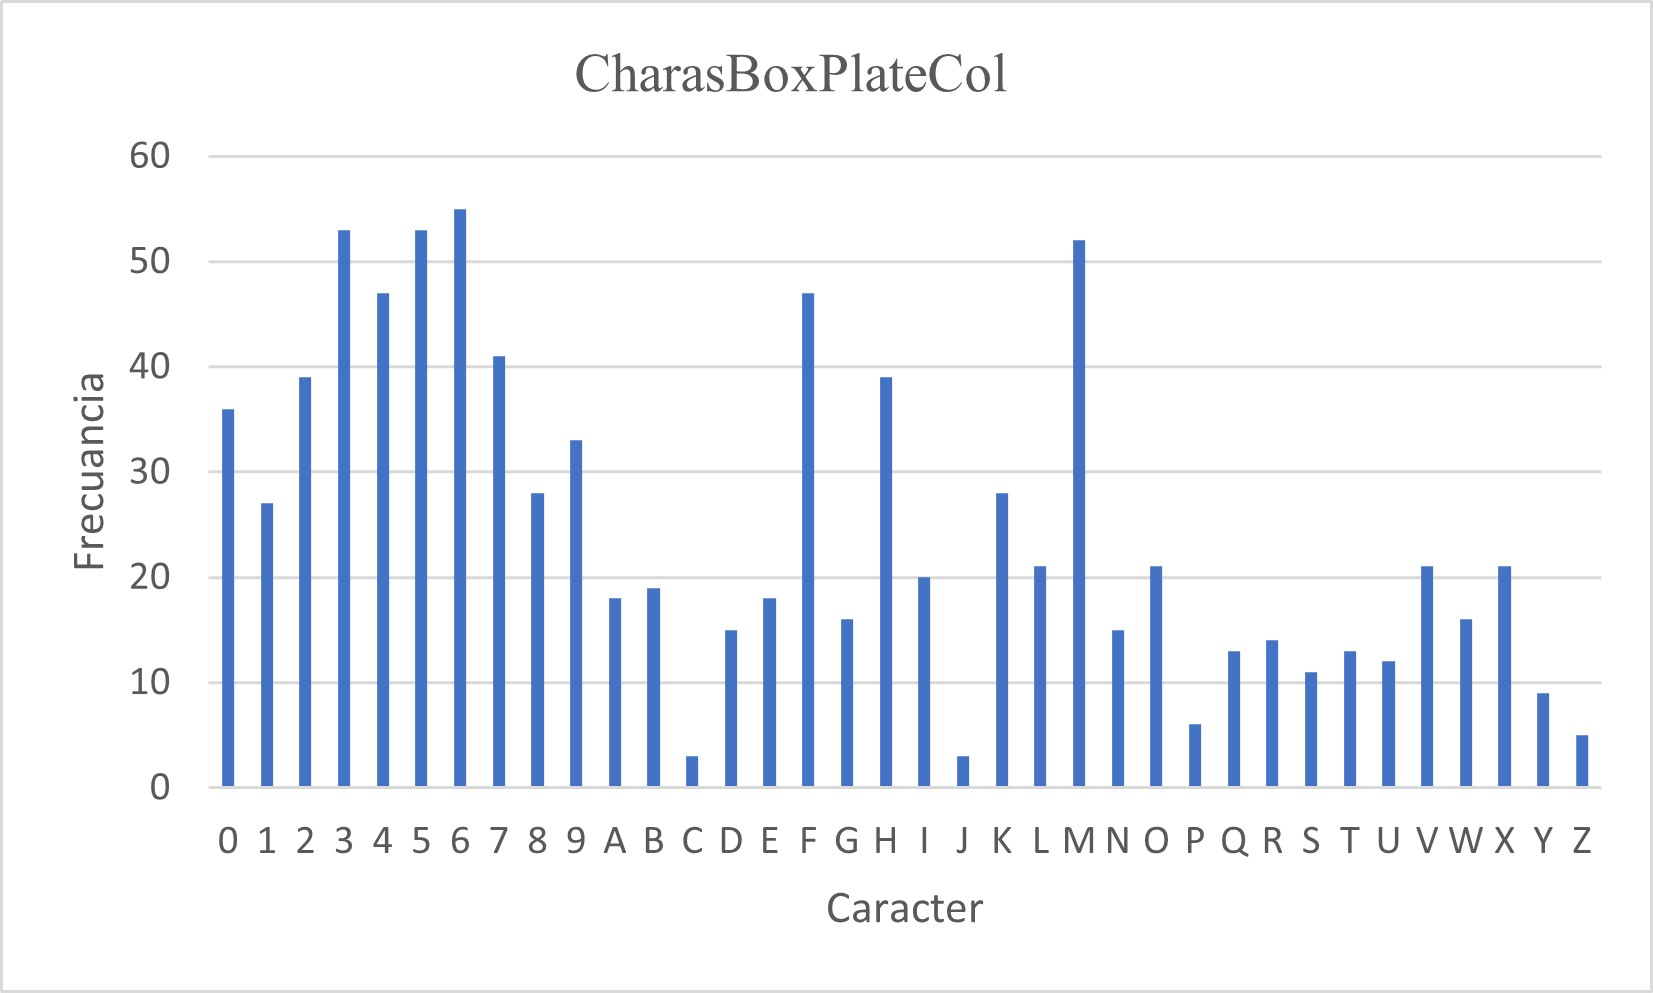
\includegraphics[width=0.8\linewidth]{imagenes/frecuenciaCaracter3.jpg}}
   \caption{Frecuencia de cada caracter en la base de datos \textit{CharsBoxPlateCol}}.
    \label{fig:frecuencia3}
\end{figure}

 \begin{tcolorbox}
[colback=green!5!white,colframe=green!45!black,fonttitle=\bfseries,title=Contribución]

   Una contribución del presente trabajo son las bases de datos \textit{CharsPlateCol} y \textit{CharsBoxPlateCol} con caracteres segmentados y etiquetados respectivamente de placas colombianas, las cuales están disponibles para cualquier investigador que las requiera para usos académicos.
\end{tcolorbox}\\

%Para tener una base de datos etiquetada con caracteres con una mayor frecuencia, se realizó una aumento de datos utilizando la aplicación RoboFlow. Ésta aplicación permite realizar muchas transformaciones de la imagen. Nosotros hemos realizado solamente cambios en el brillo (Brightness), en la rotación (Rotation), en el nivel de ruido (Noise) y en el difuminado (Blur). Estos cambios se han realizado teniendo en cuenta que se asemejan a los cambios que se pueden producir en la imagen de la placa por condiciones ambientales y por las diferentes perspectivas en que la cámara puede capturar la imagen de la placa.    
%En la tabla \ref{table:frecuencia4} se muestra la cantidad de imágenes en cada clase después de realizado el aumento de datos; y en la figura \ref{fig:frecuencia4} un diagrama de frecuencias. Se puede observar en el diagrama que se obtiene aun una base de datos muy desbalanceada, pero con mayor frecuencia en algunos caracteres.

\begin{comment}

\begin{table}[H]
\begin{center}
\resizebox{0.5\textwidth}{!}{
\begin{tabular}{||c|c||c|c||}
\hline \hline
 Clase & Frecuencia & Clase & Frecuencia\\
\hline\hline
000  &  476 & letra I  & 228 \\\hline
001  &  399 & letra J  &  83\\\hline
002  &  544 & letra K & 371\\\hline
003  & 762 & letra L & 289\\\hline
004 &  648 & letra M  & 729\\\hline
005 & 762 & letra N  &  223\\\hline
006 & 755 & letra O  & 260\\\hline
007  &  609 & letra P  &  69\\\hline
008 & 379 & letra Q & 125\\ \hline
009 & 432 & letra R & 151\\\hline
letra A  &  234 & letra S  &  119\\\hline
letra B  &  194 & letra T  &  153\\\hline
letra C  &  41 & letra U & 152\\\hline
letra D  & 211 & letra V  & 239 \\\hline
letra E  &  205 & letra W  & 186 \\\hline
letra F & 533 & letra X & 207 \\\hline
letra G  & 195 & letra Y  & 105\\\hline
letra H & 433 & letra Z  & 72\\
\hline \hline
Total etiquetas & \multicolumn{3}{|c|}{11573} \\
\hline \hline
\end{tabular}
}
\caption{\label{table:frecuencia4}Cantidad de etiquetas por clase en la base de datos \textit{CharsBoxPlateCol} con data aumentada}
\end{center}
\end{table}

\begin{figure}[H]
\centering
  {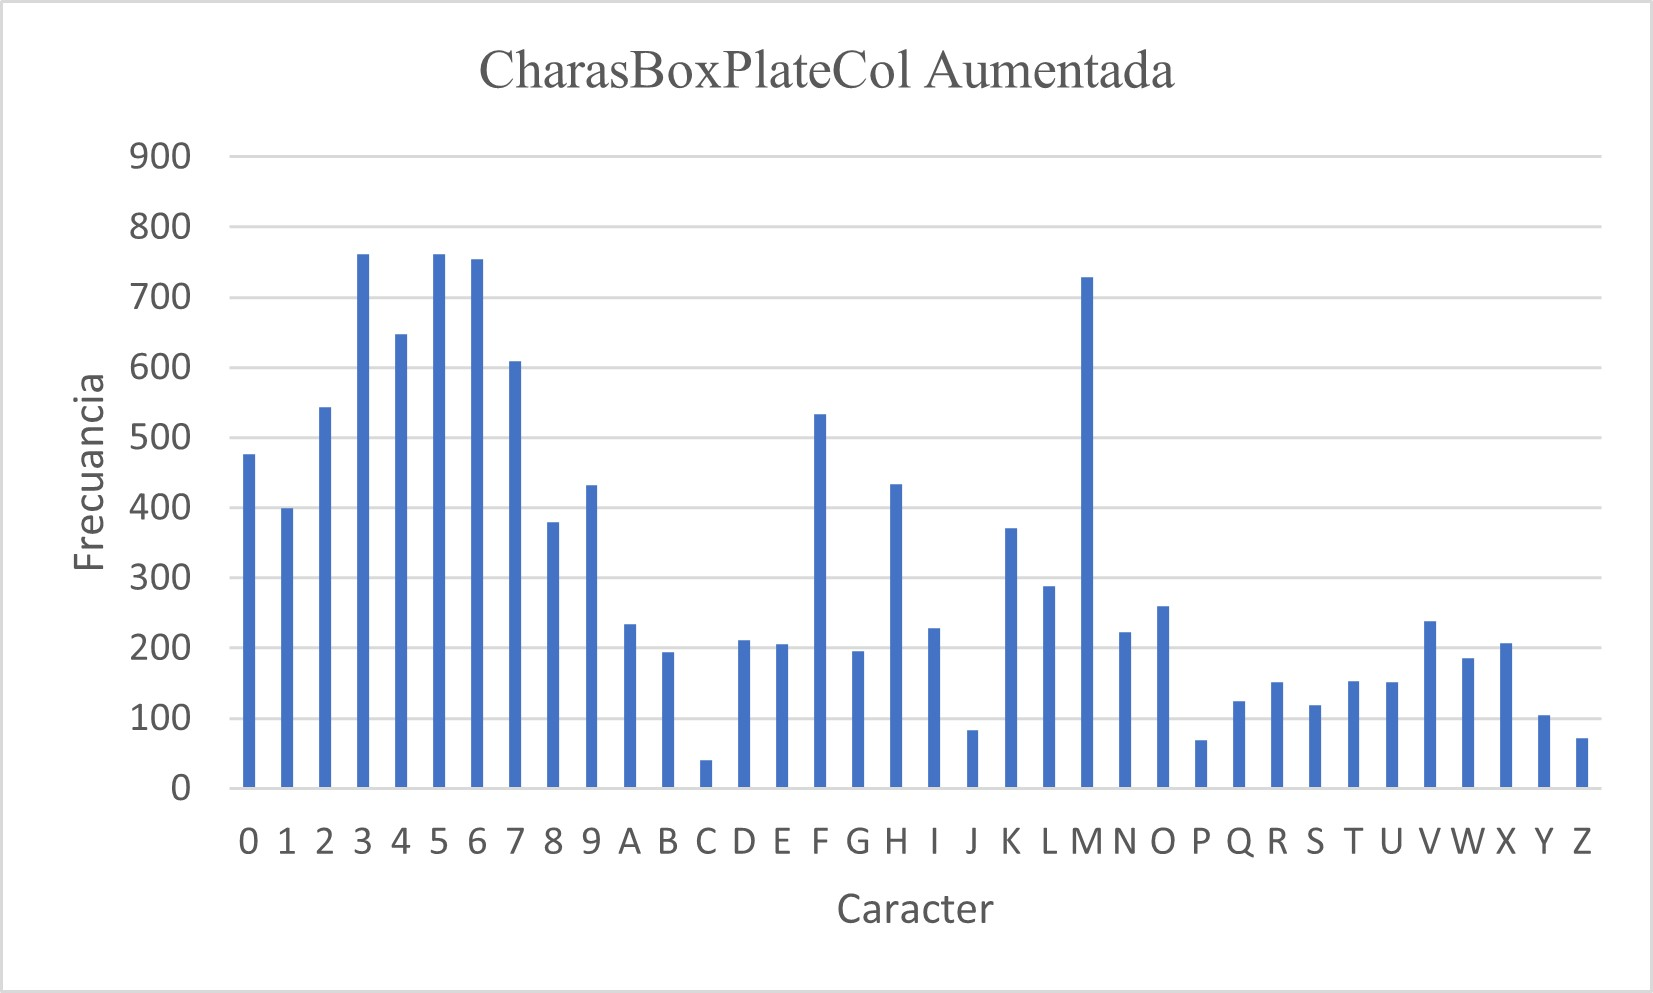
\includegraphics[width=0.7\linewidth]{imagenes/frecuenciaCaracter4.jpg}}
   \caption{Frecuencia de cada caracter en la base de datos \textit{CharsBoxPlateCol} aumentada}.
    \label{fig:frecuencia4}
\end{figure}

\end{comment}





%-----------------------------------
%La base de datos para el entrenamiento de la técnica de detección de objetos, se construye a partir de la creación de etiquetas dentro de las imágenes. Se crean cuadros delimitadores (bounding box) para cada una de las clases que se quieren detectar, independiente de la cantidad de objetos o caracteres en una misma imagen, como es nuestro caso. Por tal razón, hemos etiquetado 6 caracteres en cada una de las imágenes de la placas colombianas seleccionadas para el entrenamiento y test de nuestro modelo Faster R-CNN de tensorflow pre-entrenado.


%Se implementó una detección de objetos de tensorflow con python para el reconocimiento de caracteres en imágenes de placas vehiculares, acá es un proceso un poco diferente a la red neuronal convolucional de clasificación, ya que, en primer lugar, se detectan los 6 caracteres dentro de la misma placa que ha sido segmentada con anterioridad, lo segundo, es que hacemos una etiqueta en las imágenes que contienen la placa para el entrenamiento de la red neuronal convolucional y la construcción de la base de datos.

%Esta etapa es un pre-procesamiento de imágenes para el entrenamiento de la red neuronal convolucional mucho mas rápida con propuesta de regiones. El etiquetado se hace manualmente en los 6 caracteres en cada una de las im\'agenes predeterminadas para el entrenamiento y test, creando as'i las 36 clases que representa cada uno de los caracteres usados en las placas colombianas, esas etiquetas son cuadros delimitadores de colores por cada clase asignada.
%La etiqueta de cada uno de los caracteres dentro de la imagen de la placa se realizó con la aplicación \textbf{labelImg}, en este caso se etiquetaron 112 placas para el entrenamiento, con un promedio de 6 caracteres etiquetados por imagen, da un total de 672 etiquetas , 65 imágenes para la validación, con un promedio de 6 caracteres etiquetados para un total de 390 etiquetas\\


%\begin{figure}[H]
%\centering
%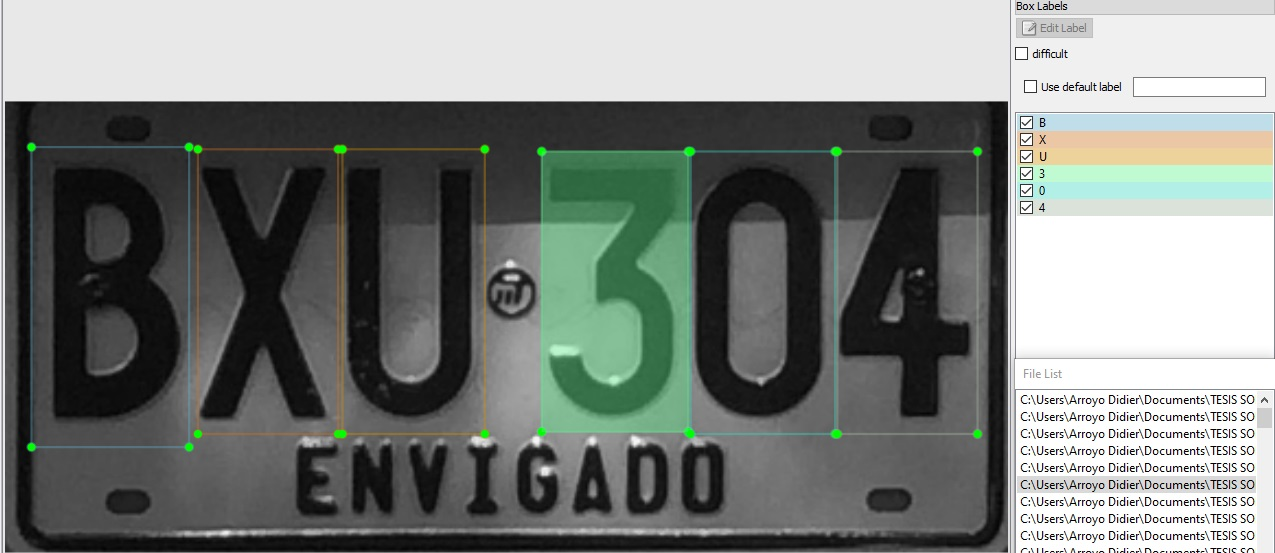
\includegraphics[width=0.5\textwidth]{imagenes/MODELO_5/ETIQUETA_MOD_IV.jpg} \caption{Caracteres etiquetados}
%\label{fig:etiquetas deteccion}
%\end{figure}

%La figura \ref{fig:etiquetas deteccion} es una muestra de las 177 placas que lograron etiquetarse, se crea un bounding box en cada clase identificada dentro de la imagen,con un color específico, este proceso genere automáticamente el documento \textbf{Xml} con las coordenadas de cada una de las clases delimitada con los cuadros.
%Este proceso se tiene que hacer manualmente con cada una de las imágenes predeterminadas para el entrenamiento de la red neuronal, donde se generará un documento \textbf{xml} por cada imagen donde se encuentran al menos unas coordenadas de las etiquetas realizadas. 

%\begin{figure}[H]
%\centering
%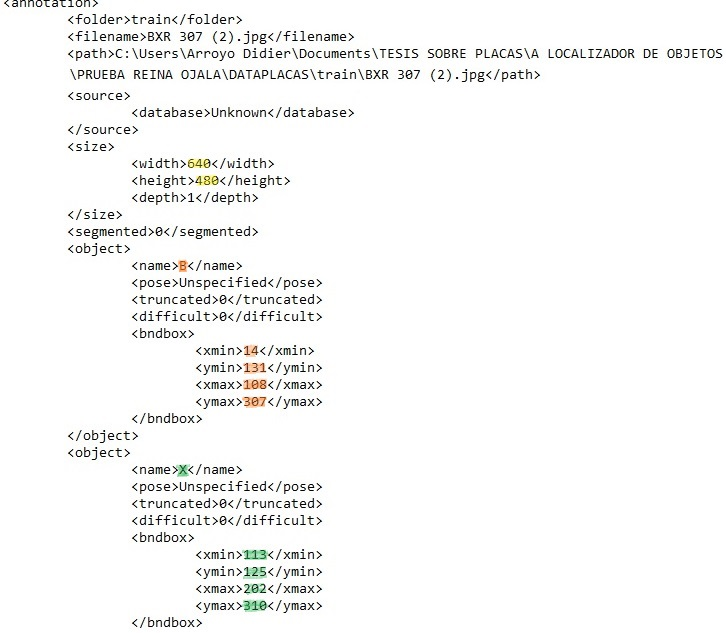
\includegraphics[width=0.7\linewidth]{imagenes/RESULTADOS/annonations.jpg} \caption{Ejemplo anotación Xml}
%\label{fig:Ejemplo anotación Xml}
%\end{figure}

%La figura \ref{fig:Ejemplo anotación Xml} es un ejemplo de la anotación de las coordenadas de las etiquetas realizadas en la imagen para la creación de la data,  en este caso podemos observar las coordenadas para las clases \textbf{B} y \textbf{X}, que gráficamente podemos observar en la figura \ref{fig:etiquetas deteccion} 

%------------------------------------------
\section{Técnicas estadísticas para el procesamiento de la información}
%---------------------------------------------------------

%La figura 5.1 muestra que la entrada del sistema son imágenes completas que incluyen vehículo y todo su contexto. Las imágenes de  entrada pertenecen a una base de datos de un parqueadero y tienen una resolución fija de 1920 x 1080. Una vez introducida una imagen, el sistema ejecutará el proceso de segmentación de la placa y luego lo hará con los caracteres que esta contiene, debemos tener en cuenta el formato de matrículas en Colombia es: tres letras y tres números. El código que realiza este primer proceso, que es la segmentación basada en la detección de contornos, se lleva a cabo con las funciones de la librería de visión artificial OpenCV.\\

En este trabajo se han usado Redes Neuronales Convolucionales para el procesamiento de la información. Consideramos que estas redes son adecuadas para superar los retos que se han planteado  en el reconocimiento de placas colombianas de automóviles, ya que presenta la ventaja de que la extracción de características viene incorporado dentro del proceso de entrenamiento de la red (ver secciones \ref{sec:antecedentes} y \ref{sec:RNC}). Nosotros hemos desarrollado dos modelos: Un primer modelo es una RNC construida desde cero e inicialmente fue entrenada utilizando solamente la base de datos \textit{CharsPlateCol} y luego fue entrenada agregándole la base de datos \textit{Chars34k}. Un segundo modelo usa la técnica de detección de objetos. Para ello hemos realizado transferencia de aprendizaje a partir de una Faster R-CNN pre-entrenada con la base de datos COCO (ver sección \ref{sec:coco}). Para entrenar la red inicialmente se usó la base de datos \textit{CharsBoxPlateCol} y después, la misma base de datos aumentada con aplicación Web RoboFlow (ver sección \ref{sec:basedatos3}).  A continuación se describen los dos modelos usados.    
%-----------------------------------------
%y  Hemos empleado en este trabajo dos técnicas para procesar la información, la primera es una Red Neuronal Convolucional 
%(RCN) la cual ser\'a la encargada del reconocimiento de caracteres en nuestro sistema después del proceso de segmentación de caracteres, igual al realizado en la creación de la data \textit{CharsPlateCol2.5k}. (ver sección \ref{CharsPlateCol2.5k}).\\ 
%La etapa de reconocimiento de caracteres realizada mediante la  red neuronal convolucional (RNC), tiene una primera fase, entrenamiento, validación y test realizado con la base de datos \textit{CharsPlateCol2.5k}, (ver sección \ref{CharsPlateCol2.5k}) para la creación de nuestro modelo 1, de igual forma entrenamos esta misma red neuronal con la base de datos \textit{Chars34k},   (Ver sección \ref{Chars34k}) para la creación de nuestro modelo 2. 
%La segunda t\'ecnica usada es la detección de objetos, se us\'o el modelo pre-entrenado de tensorflow \textbf{faster r-cnn inception v2 coco 2018 01 28} para entrenar nuestro propio clasificador de detección de objetos con una red neuronal convolucional para múltiples objetos y así poder identificar con cuadros delimitadores los caracteres en las placas colombianas, esto se hizo a partir de la técnica conocida como fine-tuning (ajuste fino).(Ver sección \ref())


%El objetivo de esta etapa es detectar aquellas regiones de la imagen que contienen los números y letras que posteriormente tratará de identificar el clasificador de la red neuronal.

%La etapa final del ejemplo de segmentación es cuando obtenemos los 6 caracteres que se extraen de toda la placa segmentada, teniendo en cuenta las dimensiones fijas de las placas colombianas. Los caracteres segmentados sirven como entrada a la red neuronal convolucional previamente entrenada, para su reconocimiento respectivo.


\subsection{Modelo 1: RNC desde cero}\label{sec:modelo1}
Este primer modelo construido desde cero consta de 3 capas de convolución seguidas de una función de activación ReLu y una capa MaxPooling. Además, una Capa de activación SoftMax con 36 salidas (26 letras y 10 números), que indican los porcentajes de clasificación obtenidos para cada clase. La tabla \ref{tab:Distribución de capas RCN} muestra su distribución de capas y parámetros.

\begin{table}[H]
    \centering
    \begin{tabular}{||c|c||}
      \hline \hline
      \textbf{Tipo de Capa} & \textbf{Cantidad}\\
      \hline \hline
      Convolucional & 5 \\
      \hline
      Densas & 3 \\
      \hline
      MaxPooling & 3 \\
      \hline
      Dropout & 2\\
      \hline
      Flatten & 1 \\
      \hline
      Total de capas & 14  \\
      \hline
      \hline
    \end{tabular}
    \caption{Distribución de capas Modelo}
    \label{tab:Distribución de capas RCN}
\end{table}

El proceso de entrenamiento de la red se basa en una estructura que relaciona unas capas convolucionales, unas capas pooling y por último una capas totalmente conectadas que nos indicará la clasificación realizada por medio de la función SoftMax.

El proceso de entrenamiento inicia con la declaración de la estructura de la red. El siguiente paso es importar el conjunto de imágenes de la base de datos. Antes de iniciar el entrenamiento, este conjunto de imágenes se divide aleatoriamente en tres subconjuntos denominados entrenamiento, validación y prueba. El conjunto de entrenamiento se utiliza para determinar los pesos de la red que permiten clasificar con el menor error posible las imágenes; el de validación para comprobar si se produce sobreajuste (\textit{overfitting}) durante el entrenamiento; y el conjunto de prueba para calcular la precisión del modelo a la hora de clasificar imágenes que no han sido utilizadas durante las épocas de entrenamiento.

El entrenamiento de esta RNC se realizó en Colaboratory \cite {Bisong2019}, un entorno gratuito de Jupyter Notebook que se ejecuta completamente en la nube.

\begin{table}[H]
\begin{center}
\begin{tabular}{||c|c|c|c||}
\hline \hline
&\textbf{Tipo de capa} & \textbf{Salida} & \textbf{No. Parámetros}\\
\hline \hline
\multirow{7}{*}{\rotatebox{90}{Ext. Características}}&\verb"conv_1(conv2D)"&(74,34,64) & 9472\\\cline{2-4}

&\verb"Activacion_1(Activacion)"& (74,34,64) & 0 \\\cline{2-4}

&\verb"pooling_1(MaxPooling2D)"&(37,17,64) &0\\\cline{2-4}

&\verb"conv_2(conv2D)"&(35,15,128) & 73856\\\cline{2-4}

&\verb"Activacion_2(Activacion)"& (35,15,128) & 0 \\\cline{2-4}

&\verb"pooling_2(MaxPooling2D)"&(17,7,128) & 0\\\cline{2-4}

&\verb"conv_3(conv2D)"&(15,5,256) & 295168\\\cline{2-4}

&\verb"Activacion_3(Activacion)""&(15,5,256) & 0 \\\cline{2-4}

&\verb"pooling_3(MaxPooling2D)"&(7,2,256) & 0\\\hline


\multirow{6}{*}{\rotatebox{90}{Clasificador}}&\verb"flatten_1(Flatten)"&(6144) & 0\\\cline{2-4}

& Dense\_1 (dense) & (1024) & 3671040 \\ \cline{2-4}
& Dropout\_1 (dropout) & (1024) & 0 \\ \cline{2-4}
& activation\_4 (activation)  & (1024) & 0 \\ \cline{2-4}
& Dropout\_2 (dropout) & (1024) & 0\\ \cline{2-4}
& Dense\_2 (dense) & (36) & 36900 \\ \cline{2-4}
& activation\_5 (Softmax) & (36) & 0\\ \hline \hline
\multicolumn{3}{||c|}{\verb"Total parámetros"}& \verb"4086436"\\
\hline
\multicolumn{3}{||c|}{\verb"Parámetros entrenables"}&\verb"4086436"\\
\hline
\multicolumn{3}{||c|}{\verb"Parámetros no entrenables"}&\verb"0"\\
\hline \hline
\end{tabular}
\caption{Estructura de la red neuronal convolucional diseñada}
\label{tab:modelo1}
\end{center}
\end{table}


\subsubsection*{Arquitectura}

Para lograr obtener una arquitectura con buen rendimiento, se realizaron varios ensayos. Inicialmente se entrenó en 50 épocas, luego se logró cambiar el entorno de entrenamiento y todos se llevaron a cabo en 200 épocas. Inicialmente el tamaño de las imágenes de entrada fueron de 32x32; luego pasaron a 50x50 y finalmente las imágenes de 80x40 píxeles con 3 canales RGB fueron las que dieron mejor resultado. Los entrenamientos se hicieron inicialmente en el entorno Jupyter en Anaconda, pero debido a la complejidad y duración excesiva de los entrenamientos (hasta 3 días), usamos el mismo entorno pero en Google Colab con acceso a trabajos con GPU totalmente gratis y en la nube. Fue así que se redujo significativamente los tiempos de entrenamiento a máximo 30 minutos. Este modelo fue entrenado con distribución de las capas descritas en el cuadro \ref{tab:Distribución de capas RCN}. La estructura de red que mejor rendimiento mostró se muestra en la tabla \ref{tab:modelo1}.

De acuerdo a la estructura de la red mostrada en la anterior tabla, cuando se tiene una imagen de entrada de 80x40 píxeles se aplica una convolución cuyo filtro es 7x7 para generar 64 mapas de características de 74x34. Un filtro de agrupación 2x2 MaxPooling se aplica a estos mapas y se obtienen 64 mapas de características de 37x17. De la misma forma lo hacemos con las siguientes convoluciones cuyos filtros son 3x3, para obtener 128 mapas de 35x15. Después de aplicar el filtro de agrupación 2x2 MaxPooling, obtenemos 128 mapas de 17x7. En la última convolución obtenemos 256 mapas de características de 15x5, que después de aplicar el filtro MaxPooling de 2x2 quedan de 7x2. Después de la etapa de extracción de características para el aprendizaje de la red, se realiza la etapa de clasificación con capas completamente conectadas. Finaliza con la función de activación Softmax, que asigna probabilidades de reconocimiento a cada una de las clases para finalmente realizar la clasificación de los caracteres en la placa de entrada.

\begin{table}[H]
\begin{center}
\begin{tabular}{||c|c||c|c||}
\hline
\hline
 Índice & clase & Índice & clase  \\
\hline
0 & letra P & 18 & letra Q\\ \hline
1 & 001 & 19 & 004\\ \hline
2 & letra O & 20 & letra U\\ \hline
3 & 008  & 21 & letra A\\ \hline
4 & letra D & 22 & 005\\ \hline
5 & letra M & 23 & letra Y\\ \hline
6 & letra N & 24 & letra L\\ \hline
7 & letra B & 25 & letra R\\ \hline
8 & 002 & 26 & letra G\\ \hline
9 & 003 & 27 & letra Z\\ \hline
10 & letra I & 28 & letra K\\ \hline
11 & letra E & 29 & letra J\\ \hline
12 & 007 & 30 & 009\\ \hline
13 & letra S & 31 & 000\\ \hline
14 & letra F & 32 & letra X\\ \hline
15 & 006 & 33 & letra V\\ \hline
16 & letra C & 34 & letra H\\ \hline
17 & letra W & 35 & letra T\\ \hline \hline

\hline
\end{tabular}
\caption{\label{table:indices_data segmentada}índices asignados a cada una de las 36 clases a clasificar}
\end{center}
\end{table}


\subsection{Entrenamiento}\label{sec:entreModelo1}

La tabla \ref{table:indices_data segmentada} muestra los índices asignados a cada una de las 36 clases a clasificar (caracteres de placas colombianas).


La tabla \ref{table:Datos de entrenamiento} muestra los parámetros utilizados para el entrenamiento del modelo 1, los cuales fueron los que dieron mejor rendimiento después de múltiples ensayos.

\begin{table}[H]
\begin{center}
\begin{tabular}{||c|c||}
\hline
 Parámetros &  \\
\hline
\hline
longitud-altura imagen & 80 x 40\\ \hline
Imágenes de entrenamiento & 1659 \\ \hline
Imágenes de validación & 415\\\hline
Imágenes de test & 519\\\hline
INIT LR & 0.001 \\\hline
épocas & 200 \\\hline
batch size & 16\\ \hline
optimizador & SGD\\\hline
\hline
\hline
\end{tabular}
\caption{\label{table:Datos de entrenamiento} Parámetros usados en el entrenamiento del Modelo 1}
\end{center}
\end{table}



\subsection{Modelo 2: Faster R-CNN pre-entrenado}

Este modelo fue construido a partir del modelo  pre-entrenado de detección de objetos \textbf{Faster R-CNN Inception v2 (COCO)} de TensorFlow.

Se realizó transferencia de aprendizaje para entrenar nuestro propio clasificador de detección de objetos, en nuestro caso, caracteres en la imagen de una placa.  La identificación se realiza con cuadros delimitadores en cada uno de los caracteres en las placas colombianas. Esto se hizo a partir de la técnica conocida como fine-tuning (ajuste fino), que consiste en realizar un ajuste de la red inicializando con los pesos ya obtenidos del modelo pre-entrenado (inferencia). En la tabla \ref{tab:Distribución de redes} se encuentra la distribución de redes y capas que conforman una \textbf{Faster R-CNN}. Está cosntituida por tres redes (RNC, RPN y R-CNN) y una capa RoIP (ver sección \ref{sec:Faster}). 

\begin{table}[H]
    \centering
    \begin{tabular}{||c|c||}
      \hline \hline
      \textbf{Tipo de red o capa} & \textbf{Cantidad}\\
      \hline \hline
      RNC & 1 \\
      \hline
      Red de propuesta de región (RPN) & 1 \\
      \hline
      Capa de agrupación de regiones de interés (RoIP)  & 1 \\
      \hline
      R-CNN & 1\\
      \hline
      Total & 4  \\
      \hline
      \hline
    \end{tabular}
    \caption{Distribución de redes y capas Modelo}
    \label{tab:Distribución de redes}
\end{table}

%Dividimos nuestra data en dos directorios train y test. El modelo solo usará imágenes del directorio "train" para entrenamiento e imágenes de la carpeta "test" para evaluar el rendimiento del modelo, luego cargamos imágenes nunca antes vista por el modelo para la prueba.
%Debemos generar dos archivos train.record y test.record, ambos son archivos binarios, cada uno contiene el jpg codificado y la información de anotación del cuadro delimitador para el conjunto de train y test correspondiente. El formato de archivo tfrecord es más fácil de usar y más rápido de cargar durante la fase de entrenamiento en comparación con el almacenamiento de cada imagen y anotación por separado. Este archivo tfrecord se genera a partir del documento \textbf{XML} que contiene las anotaciones de la etiquetas, esta información genera dos archivos, uno de los label y otro con las anotaciones de las etiquetas que finamente genere el archivo tfrecord para train y test. 
%-----------------------
%-----------------------------------------
\chapter{Resultados usando el Modelo 1\\
(RNC desde cero)}

En esta sección se presentan los resultados obtenidos al usar el modelo 1 (\ver sección \ref{sec:modelo1}). Primero se presentan los resultados del modelo 1 usando la base de datos \textit{CharsPlateCol}, luego se muestran los resultados agregándole la base de datos \textit{Chars34} y finalmente se realiza una comparación de los dos resultados.

Inicialmente se muestran resultados en la clasificación de caracteres individuales. Es decir, la imagen de entrada a reconocer es un carácter que ha sido extraído previamente de una placa colombiana. Luego, se muestran resultados en la clasificación de toda la placa. Es decir, que la imagen de entrada al sistema corresponde a la parte frontal del automóvil donde se identifica la placa (ver sección \ref{sec:basedatos3}). De esta manera el sistema de reconocimiento completo consiste en una etapa de segmentación de cada caracter en la placa y luego una etapa de reconocimiento usando la RNC previamente entrenada.  

\section{Resultado usando la base de datos\\
\textit{CharsPlateCol}}

\subsection{Reconocimiento de caracteres segmentados}

Se presentan aquí los resultados en la clasificación de caracteres individuales después de ser segmentados desde las placas. Este primer resultado se muestra con el fin de observar si el sistema de reconocimiento falla por el entrenamiento de la RNC o por el proceso de segmentación.  

Las figura \ref{fig:Progreso del entrenamiento durante 200  ́época} muestra el progreso en el rendimiento tanto del conjunto entrenamiento como en el conjunto de validación durante las 200 épocas, usando solamente la base de datos \textit{CharsPlateCol}. La figura (a) muestra el progreso en la precisión y la figura (b) en la pérdida. Se observa un distanciamiento de las dos curvas aproximadamente a partir de las 75 épocas, lo que indica un entrenamiento no muy adecuado, ya que en ese momento no se ha logrado un buen rendimiento (alta precisión y baja perdida). 

\begin{figure}[H]
  \subfigure[]{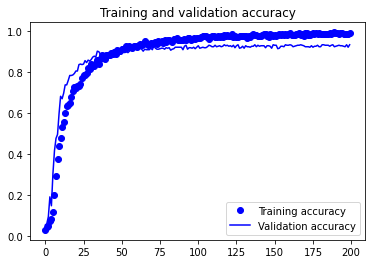
\includegraphics[width=0.5 \linewidth]{imagenes/MODEL_CARACTERES_SEGMENTADOS/ACCU.png}}
    \subfigure[]{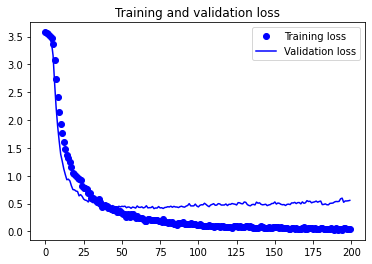
\includegraphics[width=0.5 \linewidth]{imagenes/MODEL_CARACTERES_SEGMENTADOS/LOSS.png}}
    \caption{Progreso del entrenamiento durante 200  ́épocas}
    \label{fig:Progreso del entrenamiento durante 200  ́época}  
\end{figure}


% Entrenamos a la CNN solo con caracteres segmentados y se logró un porcentaje de clasificación del 93\% en la evaluación del modelo. De las 519 imágenes del test, identificó con éxito 482, presentando dificultad en 37 de ellas. 



%En la muestra del resultado del test-modelo caracteres segmentados, podemos concluir que se presenta dificultad con caracteres con tienen algún tipo de irregularidad, ejemplo de eso, es la letra M, que es confundida por el modelo con una letra V, pero se puede comprender, ya que se evidencia que es un caracter incompleto, después de ser segmentado para crear la data de entrenamiento.  Las imágenes  (a) y (b) son una muestra de caracteres clasificados correcta e incorrectamente por el modelo.

\begin{comment}
\begin{figure}[H]
  \subfigure[]{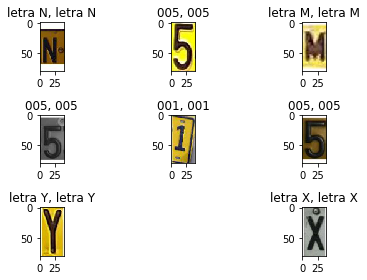
\includegraphics[width=0.4 \linewidth]{imagenes/MODEL_CARACTERES_SEGMENTADOS/CORREC_SEGMENTADAS.png}}
    \subfigure[]{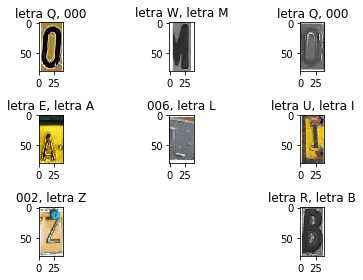
\includegraphics[width=0.4\linewidth]{imagenes/MODEL_CARACTERES_SEGMENTADOS/INCORREC_SEGMENTADA.png}}
    \caption{Resultado del test-modelo caracteres segmentados}
    \label{fig:(a) y (b) segmentada}  
\end{figure}

La figura \ref{fig:(a) y (b) segmentada} nos muestra en \textbf{(a)} 8 de las 482 caracteres clasificados correctamente en el test del modelo entrenado con la data segmentada y la imagen (b) es una muestra de 8 de los 37 caracteres clasificados incorrectamente por la red neuronal convolucional. 
\end{comment}

\subsection*{Rendimiento}

%En la figura \ref{fig:matrizconfusion1} se muestra la matriz de confusión. Podemos ver que el Modelo 1 presenta errores al momento de clasificar arrojando falso positivos y falsos negativos.

En la figura \ref{fig:matrizconfusion1} se muestra la Matriz de confusión obtenida de la evaluación del sistema usando 519 imágenes segmentadas de placas colombianas. Podemos observar en la diagonal principal el número de veces que una categoría Predicha por el modelo coincida con la Categoría verdadera. Mientras que un valor diferente de cero en las otras celdas nos indican los casos en que el modelo ha clasificado incorrectamente (Falsos Positivos y Falsos Negativos).

\begin{figure}[H]
\centering
  {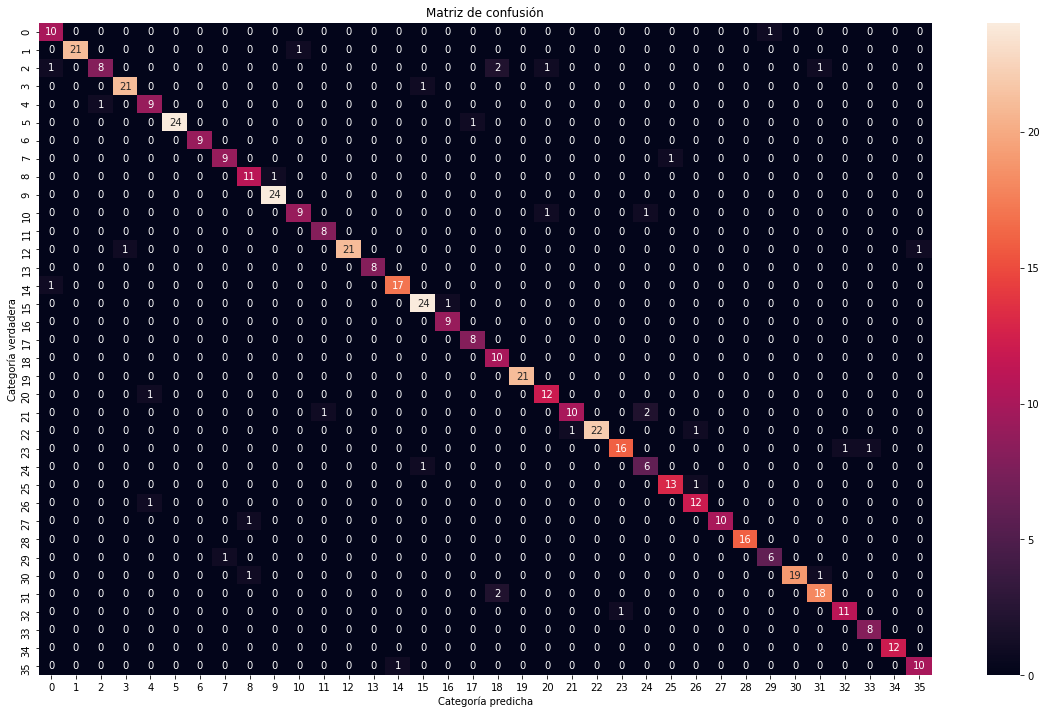
\includegraphics[width=0.7\linewidth]{imagenes/MODEL_CARACTERES_SEGMENTADOS/MATRIZ_CONFUSION.png}}
   \caption{Matriz de Confusión}
    \label{fig:matrizconfusion1}  
\end{figure}

La tabla \ref{table:Metricas segmentada} nos muestra los valores de las métricas (Precisión, Sensibilidad, valor-F1) calculados a partir de la matriz de confusión. Las métricas usadas para evaluar el Modelo 1 son el promedio ponderado de tales métricas, ya que la base de datos usada para el entrenamiento es desequilibrada (ver sección \ref{CharsPlateCol2.5k}). 

\begin{table}[H]
\begin{center}
\resizebox{0.4\textwidth}{!}{
\begin{tabular}{||c|c|c|c|c||}
\hline \hline
 Clases & Precisión &  Sensibilidad & Valor F &  Soporte\\
\hline \hline
     Clase 0 & 0.83 & 0.91 & 0.87 &  11\\\hline
     Clase 1 & 1.00 & 0.95 & 0.98 &  22\\\hline
     Clase 2 & 0.89 & 0.62 & 0.73 &  13\\\hline
     Clase 3 & 0.95 & 0.95 & 0.95 &  22\\\hline
     Clase 4 & 0.82 & 0.90 & 0.86 &  10\\\hline
     Clase 5 & 1.00 & 0.96 & 0.98 &  25\\\hline
     Clase 6 & 1.00 & 1.00 & 1.00 &   9\\\hline
     Clase 7 & 0.90 & 0.90 & 0.90 &  10\\\hline
     Clase 8 & 0.85 & 0.92 & 0.88 &  12\\\hline
     Clase 9 & 0.96 & 1.00 & 0.98 &  24\\\hline
    Clase 10 & 0.90 & 0.82 & 0.86 &  11\\\hline
    Clase 11 & 0.89 & 1.00 & 0.94 &   8\\\hline
    Clase 12 & 1.00 & 0.91 & 0.95 &  23\\\hline
    Clase 13 & 1.00 & 1.00 & 1.00 &   8\\\hline
    Clase 14 & 0.94 & 0.94 & 0.94 &  18\\\hline
    Clase 15 & 0.92 & 0.96 & 0.94 &  25\\\hline
    Clase 16 & 0.90 & 1.00 & 0.95 &   9\\\hline
    Clase 17 & 0.89 & 1.00 & 0.94 &   8\\\hline
    Clase 18 & 0.71 & 1.00 & 0.83 &  10\\\hline
    Clase 19 & 1.00 & 1.00 & 1.00 &  21\\\hline
    Clase 20 & 0.86 & 0.92 & 0.89 &  13\\\hline
    Clase 21 & 0.91 & 0.77 & 0.83 &  13\\\hline
    Clase 22 & 1.00 & 0.92 & 0.96 &  24\\\hline
    Clase 23 & 0.94 & 0.89 & 0.91 &  18\\\hline
    Clase 24 & 0.67 & 0.86 & 0.75 &   7\\\hline
    Clase 25 & 0.93 & 0.93 & 0.93 &  14\\\hline
    Clase 26 & 0.86 & 0.92 & 0.89 &  13\\\hline
    Clase 27 & 1.00 & 0.91 & 0.95 &  11\\\hline
    Clase 28 & 1.00 & 1.00 & 1.00 &  16\\\hline
    Clase 29 & 0.86 & 0.86 & 0.86 &   7\\\hline
    Clase 30 & 1.00 & 0.90 & 0.95 &  21\\\hline
    Clase 31 & 0.90 & 0.90 & 0.90 &  20\\\hline
    Clase 32 & 0.92 & 0.92 & 0.92 &  12\\\hline
    Clase 33 & 0.89 & 1.00 & 0.94 &   8\\\hline
    Clase 34 & 1.00 & 1.00 & 1.00 &  12\\\hline
    Clase 35 & 0.91 & 0.91 & 0.91 &  11\\\hline
\hline
    Exactitud &  & & 0.93  &  519\\\hline
   Macropromedio  &  0.92  &  0.93  &  0.92  &  519\\\hline
Promedio ponderado & \textcolor{red}{0.93}  &  \textcolor{red}{0.93}   & \textcolor{red}{0.93}  &  519\\
\hline
\hline
\end{tabular}
}
\caption{\label{table:Metricas segmentada}Métricas de rendimiento}
\end{center}
\end{table}

\subsection*{Análisis}
De acuerdo a la tabla \ref{table:Metricas segmentada} y la definición de las métricas consignadas en ella, se puede realizar el siguiente análisis:

Para evaluar el rendimiento de la red en la identificación de categorías por medio de imágenes que nunca fueron usadas para el entrenamiento utilizamos la métrica \textit{Valor-F} (ver sección: \ref{sec:metricas1}).

En la tabla \ref{table:Metricas segmentada} se muestran los valores del Valor-F obtenidos por cada una de las categorías obteniendo un Promedio Ponderado Valor-F de 0,93.\\ 

\begin{tcolorbox}
[colback=blue!5!white,colframe=blue!45!black,fonttitle=\bfseries,title=Conclusión]
   El modelo tiene un rendimiento del 93\% en reconocer categorías con imágenes que nunca fueron usadas para el entrenamiento de la red neuronal convolucional.
\end{tcolorbox}\\
\\
Ahora analizaremos que tanto el sistema logra reconocer un mismo caracter con características muy diferentes por el proceso de segmentación, deterioro de la placa o condiciones ambientales externas, teniendo en cuenta que este tipo de caracteres es muy común en este problema.

Así que Las imágenes de un mismo caracter pueden presentar característica diferentes por las razones descritas anteriormente. Todos estos factores pueden ocasionar que el sistema reporte falsos negativos.  

Para evaluar el rendimiento de la red en el reconocimiento de una misma categoría aunque sus imágenes presenten características diferentes usamos la métrica \emph{Sensibilidad} (ver sección: \ref{sec:metricas1}), ya que ésta sirve para evaluar qué tanto el sistema evita los falsos negativos.

En la tabla \ref{table:Metricas segmentada} se muestran los valores de la Sensibilidad obtenidos por cada una de las categorías obteniendo un Promedio Ponderado de la Sensibilidad de 0,93. \\
\begin{tcolorbox}
[colback=blue!5!white,colframe=blue!45!black,fonttitle=\bfseries,title=Conclusión]
   El modelo tiene un rendimiento del 93\% en reconocer un mismo caracter aunque se le presente en imágenes con características muy diferentes.
\end{tcolorbox}\\

Finalmente analizamos el resultado de la discriminación entre categorías diferentes con características similares. Es detallar que tanto el sistema logra aprender a discriminar entre dos caracateres como la \textbf{Letra Q/Letra O}, que presentan características muy similares.  Las imágenes de dos caracteres diferentes pueden presentar característica muy similares debido principalmente a su forma. Algunas veces, una la perspectiva o grado de inclinación del caracter puede generar una similitud con otro caracter, letra M/letra N. Todos estos factores pueden ocasionar que el sistema reporte falsos positivos.

Para evaluar el rendimiento de la red cuando se le presentan imágenes de distintos caracteres pero con características similares usamos la métrica Precisión (ver \ref{sec:metricas1}), ya que ésta sirve para evaluar qué tanto el modelo evita los falsos positivos.

En la tabla \ref{table:Metricas segmentada} se muestran los valores de la Precisión obtenidos por cada una de las categorías obteniendo un Promedio Ponderado de la Precisión de 0,93.\\

\begin{tcolorbox}
[colback=blue!5!white,colframe=blue!45!black,fonttitle=\bfseries,title=Conclusión]
   El modelo tiene un rendimiento del 93\% en discriminar entre categorías diferentes aunque se le presenten imágenes con características muy similares.
\end{tcolorbox}\\

%De acuerdo al Promedio Ponderado de la Precisión, el Modelo 1 detecta en un 93\% los casos positivos. De acuerdo al Promedio Ponderado de la 

%A pesar de tener una base de datos con pocas imágenes, obtuvimos buenos resultados en el promedio promedio Precisión (93\%). Aunque, para el uso que se le quiere dar al sistema de reconocimiento de placas (acceso y seguridad), este valor no es aceptable. 

%En cuanto a la exactitud del modelo, logramos un porcentaje del 93\% valor que tampoco es aceptable, nuestro objetivo es un valor mayor o igual al 99\%. 


%En cuanto a F1-score podemos concluir que nuestro modelo en algunas clases como la 2, ses confiable al momento de detectar la clase, a pesar de su dificultad al hacerlo, esto teniendo en cuenta que maneja una alta precisión y bajo recall, en el caso de la clase 24, es totalmente diferente, tenemos baja precisión y alto recall, lo que indica que el modelo detecta bien la clase, pero también incluye frecuentemente muestras de otras clases, lo mismo sucede con la clase 18. Debemos resaltar que tenemos clases que son manejadas perfectamente por el modelo, como la 6, 13, 19, 28 y 34.

\subsection{Reconocimiento de toda la placa}

Con el modelo entrenado para el reconocimiento de caracteres de placas Colombianas, colocamos a prueba todo el sistema, iniciando con el cargue de la imagen de entrada y todo el proceso de segmentación. (Ver sección \ref{fig:segmentación de caracteres}). La segmentación nos arroja los 6 caracteres que ser\'an la entrada uno por uno de la red neuronal convolucional, figura \ref{fig:segmentación de caracteres1}. El reconocimiento de los 6 caracteres hecho por la RNC se evidencia en la figura \ref{fig:Resultado del reconocimiento de caracteres charscolplate3.5k} 

\begin{figure}[H]
\centering
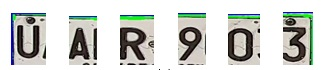
\includegraphics[width=0.7\linewidth]{imagenes/MODELO_4/segmentacion/segmentacion_figura2.jpg} \caption{segmentación de caracteres}
\label{fig:segmentación de caracteres1}
\end{figure}


\begin{figure}[H]
\centering
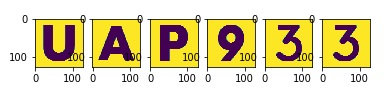
\includegraphics[width=0.9\linewidth]{imagenes/RESULTADOS/resultados_data_segmen.jpg} \caption{Resultado obtenido con una red neuronal convolucional para el reconocimiento de caracteres}
\label{fig:Resultado del reconocimiento de caracteres charscolplate3.5k}
\end{figure}

El modelo entrenado con la data segmentada, tiene inconvenientes en el reconocimiento de algunos caracteres, en este caso, se presenta dificultad al reconocer la letra \textbf{R} y el número \textbf{0}, que los confunde con la letra \textbf{P} y el número \textbf{3} respectivamente.

En general, el sistema de reconocimiento ha tenido mínimas fallas con letras que no tienen muchas imágenes en la data, como la letra H, que en pocos casos no logró reconocerla y la confundió con la letra T, igual sucede con la letra X cuando está incompleta después de la segmentación, la confunde con la letra K, pero ha sucedido con placas que tienen mucho brillo, aunque el problema radica en la segmentación, ya que tenemos placas desde diferentes perspectivas lo que implica un recorte diferente en cada caso y lleva al modelo a reconocer caracteres incompletos lo que hace que lo confunda con otro caracter. Los caracteres bien segmentados no han tenido inconvenientes al ser reconocidos, al igual que los caracteres incompletos, sino que en algunos casos tiene dificultad.

\section{Resultado usando la base de datos\\
\textit{CharsPlateCol} más la base de datos\\
\textit{{Chars34k}}}

\subsection{Reconocimiento de caracteres segmentados}
%La red neuronal ha sido entrenada nuevamente debido a la dificultad de clasificar algunos caracteres después del proceso de segmentación y entrenamiento con el modelo 1. En este ocasión hemos usado la data \textit{Chars34k} unida con la data \textit{charsplatecol2.5K}, para un total de 37.398 imágenes de 40 x 80 píxeles, que usaremos para el entrenamiento de la red neuronal convolucional bajo las mismas condiciones que el anterior entrenamiento, la diferencia será el uso de esta nueva data. La nueva data cuenta con un caracteres por clase en promedio 1000 imágenes. la letra \textbf{Q} es el caracter con el menor número, 886 y la letra \textbf{X} cuenta con exactamente 2065 imágenes. Ver cuadro \ref{table:imagenes por clase chars74k}\\


Los datos relacionados a continuación, son muy importantes para el entrenamiento de nuestra red convolucional, píxeles de las imágenes, cantidad de imágenes para el entrenamiento, validación y el test, el optimizador usado, entre otras. Tabla \ref{table:Hiperparametros Chars74K}

\begin{table}[H]
\begin{center}
\begin{tabular}{||c|c||}
\hline \hline
 Parámetros &  \\
\hline \hline
longitud-altura imagen & 80 x 40\\\hline
Imágenes de entrenamiento & 26253 \\ \hline
Imágenes de validación & 7405\\\hline
Imágenes de test & 3721\\\hline
INIT LR & 0.001 \\\hline
épocas & 200 \\\hline
batch size & 16\\ \hline
optimizador & SGD\\
\hline
\hline
\end{tabular}
\caption{\label{table:Hiperparametros Chars74K} Datos de entrenamiento}
\end{center}
\end{table}

%La red neuronal diseñada para el reconocimiento de caracteres de las placas colombianas de automóviles consta de 3 capas de convolución seguidas de una función de activación RELU y una capa maxpooling, luego tiene capas flatten, dense, dropout cerrando con una capa de activación softmax con 36 salidas, que nos indicará los porcentajes de clasificación obtenidos para cada clase. la estructura de esta red se muestra en la tabla \ref{table:estructura CNN}

%Cuando tenemos una imagen de entrada de 80x40 píxeles se le aplica una convolución cuyo filtro es 7x7 para generar 64 mapas de características de 74x34. A estos mapas se les aplica el filtro Max pooling de 2x2 y se obtienen mapas de características de 37x17. De igual forma hacemos con las siguientes convoluciones cuyos filtros son de 3x3, para obtener 128 mapas de 35x15, Luego del filtro Max pooling de 2x2, obtenemos mapas de 128 de 17x7. En la última convolución obtenemos 256 mapas de características de 15x5, que después del filtro Max pooling de 2x2 quedan de 7x2. Después de la etapa de extracción de características para el aprendizaje de la red, se realiza la clasificación a partir del flatten, dropout y la capa fully connected. Se finaliza con la función softmax, la cual asigna probabilidades a cada una de las clases al momento de realizar la clasificación. 

%La red neuronal entrenada recibe cada uno de los 6 caracteres segmentados y realiza su proceso de clasificación de acuerdo al entrenamiento realizado previamente. 

%En la primera etapa, se ha logrado segmentar en cada una de las placas, sus 6 caracteres con una efectividad de 98\%. En algunos casos el caracter queda al limite del recorte, y puede dificultar su correcta clasificación. El entrenamiento de la CNN se realizó en Colaboratory, un entorno gratuito de Jupyter Notebook que se ejecuta completamente en la nube. Entrenando la CNN solamente con caracteres de chars74K se obtuvo un porcentaje de clasificación de caracteres individuales que no superaba el 90\%. Pero, incluyendo para el entrenamiento las imágenes de caracteres segmentados de placas colombianas se logró un porcentaje del 99,49\% en la evaluación del modelo. De las 3.740 imágenes logró identificar correctamente 3.721, presentando dificultad en 19 de ellas. La figura \ref{fig:progreso del entrenamiento durante 200 épocas} muestra el progreso en el entrenamiento en cuanto a accuracy y loss respectivamente durante 200 épocas. 

Las figura \ref{fig:progreso del entrenamiento durante 200 épocas modelo2} muestra el progreso en el rendimiento tanto del conjunto entrenamiento como en el conjunto de validación durante las 200 épocas, usando la base de datos \textit{CharsPlateCol mas chars34k}. La figura (a) muestra el progreso en la precisión y la figura (b) en la pérdida. Se observa un buen comportamiento de la dos curvas que se ajustan a la curva del entrenamiento durante las 200 épocas, lo que indica un entrenamiento muy adecuado, ya que ha logrado un buen rendimiento (alta precisión y baja perdida). 

\begin{figure}[H]
  \subfigure[]{\includegraphics[width=0.5\linewidth]{imagenes/MODELO_4/ACCU_MOD_IV.jpg}}
    \subfigure[]{\includegraphics[width=0.5\linewidth]{imagenes/MODELO_4/LOSS_MOD_IV.jpg}}
    \caption{progreso del entrenamiento durante 200 épocas}
    \label{fig:progreso del entrenamiento durante 200 épocas modelo2}  
\end{figure}

\begin{comment}

En la muestra de los Resultados del test del modelo entrenado con la data \textit{Chars34K} más Data \textit{charsPlateCol2.5k}, nos enfocamos en los caracteres clasificados incorrectamente, concluyendo que algunos de esos caracteres tienen un nivel de dificultad bastante alto, como es el caso de la \textbf{letra J}, que además de tener un color gris está significativamente inclinada, la \textbf{letra o} está bastante pixelada, lo que indicaría que es la razón para ser confundida con una \textbf{letra p }

podemos concluir que se presenta dificultad con caracteres que tienen algún tipo de irregularidad, ejemplo de eso, es la letra M, que es confundida por el modelo con una letra V, pero se puede comprender, ya que se evidencia que es un caracter incompleto, después de ser segmentado para crear la data de entrenamiento.  En la figura \ref{fig:(a) y (b)} (a) y (b) son una muestra de caracteres clasificados correcta e incorrectamente por el modelo.

\begin{figure}[H]
  \subfigure[]{\includegraphics[width=0.5\linewidth]{imagenes/MODELO_4/CLASIF_MOD_IV.jpg}}
    \subfigure[]{\includegraphics[width=0.5\linewidth]{imagenes/MODELO_4/NO_CLASIF_MOD_IV.jpg}}
    \caption{Resultados del test, modelo entrenado \textit{Chars34K} más Data \textit{CharsPlateCol2.5k}}
    \label{fig:(a) y (b)}  
\end{figure}

La figura \ref{fig:(a) y (b)} nos muestra en \textbf{(a)} 8 de las 3721 caracteres clasificados correctamente en el test del modelo entrenado con la data chars74K más data segmentada y la imagen (b) es una muestra de 8 de los 19 caracteres clasificados incorrectamente por la red neuronal convolucional. 
\end{comment}

\subsection*{Rendimiento}

En la figura \ref{fig:matriz de confusion chars74k más data} se muestra la Matriz de confusión obtenida de la evaluación del sistema usando 3740 imágenes segmentadas de placas colombianas y de la base de datos \textit{chars34k} escogidas aleatoriamente. Podemos observar en la diagonal principal el número de veces que una categoría Predicha por el modelo coincida con la Categoría verdadera. Mientras que un valor diferente de cero en las otras celdas nos indican los casos en que el modelo ha clasificado incorrectamente (Falsos Positivos y Falsos Negativos).

\begin{figure}[H]
\centering
  {\includegraphics[width=0.5\linewidth]{imagenes/MODELO_4/matriz_de_confusion.png}}
  \caption{Matriz de confusión modelo Chars74K más Data Segmentada}
   \label{fig:matriz de confusion chars74k más data}  
\end{figure}

La tabla \ref{table:Metricas chars74k más data} muestra los valores de las métricas utilizadas para evaluar el rendimiento del modelo. En general, podemos observar que las métricas del modelo son muy buenas ya que se logra una  Exactitud del 99,49\%; un valor muy próximo al 100\% que nos indica  la cantidad de predicciones positivas que fueron correctas. 

Para evaluar el rendimiento general de la red en la identificación de categorías por medio de imágenes que nunca fueron usadas para el entrenamiento utilizamos la métrica \textit{Valor-F} (ver sección: \ref{sec:metricas1}).

El PP Valor-F es de 0,9949,  en este caso podemos afirmar que nuestro modelo maneja perfectamente cada clase, ya que tenemos valores de alta precisión y alta Sensibilidad. Además, podemos observar que tenemos 13 clases reconocidas 100\% por nuestro modelo.\\

 \begin{tcolorbox}
[colback=blue!5!white,colframe=blue!45!black,fonttitle=\bfseries,title=Conclusión]
   El modelo tiene un rendimiento del 99,49\% en reconocer categorías con imágenes que nunca fueron usadas para el entrenamiento de la red neuronal convolucional.
\end{tcolorbox}\\

\newpage

\begin{table}[H]
\begin{center}
\resizebox{.5\textwidth}{!}{
\begin{tabular}{||c|c|c|c|c||}
\hline \hline
 Clases & Precisión  &  Sensibilidad & Valor F  & Soporte\\
\hline \hline
Clase 0  &   1.0000 &   0.9894 &   0.9947  &   94\\\hline
Clase 1  &   0.9919 &   0.9839 &   0.9879  &   124\\\hline
Clase 2  &   1.0000 &   1.0000 &   1.0000  &   4\\\hline
Clase 3  &   1.0000 &   0.9918 &   0.9959  &   122\\\hline
Clase 4  &   0.9891 &   1.0000 &   0.9945  &   91\\\hline
Clase 5  &   1.0000 &   1.0000 &   1.0000  &   115\\\hline
Clase 6  &   1.0000 &   0.9888 &   0.9944  &   89\\\hline
Clase 7  &   1.0000 &   0.9778 &   0.9888  &   90\\\hline
Clase 8  &   0.9904 &   0.9904 &   0.9904  &   104\\\hline
Clase 9  &   0.9913 &   1.0000 &   0.9956  &   114\\\hline
Clase 10  &   0.9545 &   0.9767 &   0.9655  &   86\\\hline
Clase 11  &   0.9908 &   0.9908 &   0.9908  &   109\\\hline
Clase 12  &   1.0000 &   1.0000 &   1.0000  &   130\\\hline
Clase 13  &   1.0000 &   1.0000 &   1.0000  &   115\\\hline
Clase 14  &   1.0000 &   1.0000 &   1.0000  &   99\\\hline
Clase 15  &   0.9912 &   0.9912 &   0.9912  &   113\\\hline
Clase 16  &   0.9885 &   1.0000 &   0.9942  &   86\\\hline
Clase 17  &   1.0000 &   1.0000 &   1.0000  &   94\\\hline
Clase 18  &   0.9896 &   0.9794 &   0.9845  &   97\\\hline
Clase 19  &   0.9909 &   0.9820 &   0.9864  &   111\\\hline
Clase 20  &   1.0000 &   0.9908 &   0.9954  &   109\\\hline
Clase 21  &   1.0000 &   1.0000 &   1.0000  &   98\\\hline
Clase 22  &   1.0000 &   1.0000 &   1.0000  &   115\\\hline
Clase 23  &   0.9794 &  1.0000  &  0.9896   &   95\\\hline
Clase 24  &   0.9908 &   1.0000 &   0.9954  &   108\\\hline
Clase 25  &   1.0000 &   1.0000 &   1.0000  &   88\\\hline
Clase 26  &   0.9891 &   0.9785 &   0.9838  &   93\\\hline
Clase 27  &   0.9694 &   1.0000 &   0.9845  &   95\\\hline
Clase 28  &   0.9907 &   1.0000 &   0.9953  &   107\\\hline
Clase 29  &   0.9912 &   0.9825 &   0.9868  &   114\\\hline
Clase 30  &   1.0000 &   1.0000 &   1.0000  &   114\\\hline
Clase 31  &   0.9957 &   0.9957 &   0.9957  &   232\\\hline
Clase 32  &   0.9897 &   0.9796 &   0.9846  &   98\\\hline
Clase 33  &   0.9897 &   0.9897 &   0.9897  &   97\\\hline
Clase 34  &   1.0000 &   1.0000 &   1.0000  &   103\\\hline
Clase 35  &   1.0000 &   1.0000 &   1.0000  &   87\\\hline
\hline
Exactitud  &  &  & 0.9949  &   3740\\\hline
Macropromedio &   0.9932 &   0.9933 &   0.9949  &   3740\\\hline
Promedio Ponderado  & \textcolor{red}{0.9934} &   \textcolor{red}{0.9933} &  \textcolor{red}{ 0.9949}  &   3740\\\hline
\hline
\end{tabular}
}
\caption{\label{table:Metricas chars74k más data}Métricas entrenamiento Chars74K más Data Segmentada}
\end{center}
\end{table}



%En la tabla \ref{table:Metricas chars74k más data} se muestran los valores del Valor-F obtenidos por cada una de las categorías obteniendo un Promedio Ponderado Valor-F de 0,9949. 

   % \begin{tcolorbox}
%[colback=blue!5!white,colframe=blue!45!black,fonttitle=\bfseries,title=Conclusión 1]
 %  El modelo tiene un rendimiento del 99,49\% en reconocer categorías con imágenes que nunca fueron usadas para el entrenamiento de la red neuronal convolucional.
%\end{tcolorbox}\\
%\\
Ahora analizaremos que tanto el sistema logra reconocer un mismo caracter con características muy diferentes por el proceso de segmentación, deterioro de la placa o condiciones ambientales externas, teniendo en cuenta que este tipo de caracteres es muy común en este problema. Así que, las imágenes de un mismo caracter pueden presentar característica diferentes por las razones descritas anteriormente. Todos estos factores pueden ocasionar que el sistema reporte falsos negativos. Para evaluar el rendimiento de la red en el reconocimiento de una misma categoría aunque sus imágenes presenten características diferentes usamos la métrica \emph{Sensibilidad} (ver sección: \ref{sec:metricas1}), ya que ésta sirve para evaluar qué tanto el sistema evita los falsos negativos. 
En la tabla \ref{table:Metricas chars74k más data} se muestran los valores de la Sensibilidad obtenidos por cada una de las categorías obteniendo un Promedio Ponderado de la Sensibilidad de 0,9933. \\

\begin{tcolorbox}
[colback=blue!5!white,colframe=blue!45!black,fonttitle=\bfseries,title=Conclusión]
   El modelo tiene un rendimiento del 99,33\% en reconocer un mismo caracter aunque se le presente en imágenes con características muy diferentes.
\end{tcolorbox}\\

Finalmente analizamos el resultado de la discriminación entre categorías diferentes con características similares. Es detallar que tanto el sistema logra aprender a discriminar entre dos caracteres como la \textbf{Letra Q/Letra O}, que presentan características muy similares.  Las imágenes de dos caracteres diferentes pueden presentar característica muy similares debido principalmente a su forma. Algunas veces, una la perspectiva o grado de inclinación del caracter puede generar una similitud con otro caracter, letra M/letra N. Todos estos factores pueden ocasionar que el sistema reporte falsos positivos.

Para evaluar el rendimiento de la red cuando se le presentan imágenes de distintos caracteres pero con características similares usamos la métrica Precisión (ver \ref{sec:metricas1}), ya que ésta sirve para evaluar qué tanto el modelo evita los falsos positivos.

En la tabla \ref{table:Metricas chars74k más data} se muestran los valores de la Precisión obtenidos por cada una de las categorías obteniendo un Promedio Ponderado de la Precisión de 0,9934.\\

\begin{tcolorbox}
[colback=blue!5!white,colframe=blue!45!black,fonttitle=\bfseries,title=Conclusión 3]
   El modelo tiene un rendimiento del 99,34\% en discriminar entre categorías diferentes aunque se le presenten imágenes con características muy similares.
\end{tcolorbox}\\

\subsection{Reconocimiento de toda la placa}

Con el modelo entrenado para el reconocimiento de caracteres de placas Colombianas, colocamos a prueba todo el sistema. La entrada es toda la imagen del vehiculo con la placa para comenzar con el proceso de segmentación. (Ver sección \ref{fig:segmentación de caracteres}). La segmentación nos arroja los 6 caracteres que ser\'an la entrada uno por uno de la red neuronal convolucional, tal como se muestra en la figura \ref{fig:segmentación de caracteres} y el resultado del reconocimiento de los 6 caracteres, realizado por la RNC, se muestra en la figura \ref{fig:Resultado obtenido con una red neuronal convolucional para el reconocimiento de caracteres chars34k} 


\begin{figure}[H]
\centering
\includegraphics[width=0.7\linewidth]{imagenes/MODELO_4/segmentacion/segmentacion_figura2.jpg} \caption{segmentación de caracteres}
\label{fig:segmentación de caracteres}
\end{figure}

\begin{figure}[H]
\centering
\includegraphics[width=0.9\linewidth]{imagenes/MODELO_4/segmentacion/resultado_carro4.jpg} \caption{Resultado obtenido con una red neuronal convolucional para el reconocimiento de caracteres}
\label{fig:Resultado obtenido con una red neuronal convolucional para el reconocimiento de caracteres chars34k}
\end{figure}

\begin{tcolorbox}
[colback=blue!5!white,colframe=blue!45!black,fonttitle=\bfseries,title=Conclusión]

Teniendo en cuenta el rendimiento de todo el sistema, podemos evidenciar la mejora al momento de reconocer los 6 caracteres de la misma placa , haciendo uso en este caso de la red neuronal convolucional entrenada con la Data \textit{Chars34K} más Data \textit{charsPlateCol}, donde logra reconocer el 100\% de los caracteres. Si el análisis lo relacionamos con las métricas, la exactitud en el modelo de la data \textit{charsPlateCol} es de 0.93 y en el modelo que se complementa con la data \textit{Chars34K} obtiene una exactitud del 0.9949. Debemos tener presente que esta Red neuronal convolucional para la clasificación, fue construida desde cero, iniciando sus entrenamientos con otros datas públicas(perros, gatos, leones) y finalizando con las data de caracteres, así mismo se diseño y construyó la base de datos para caracteres segmentados, que posteriormente fue usada para el entrenamiento en las dos RNC propuestas anteriormente.


\begin{table}[H]
\begin{center}
\resizebox{.9\textwidth}{!}{
\begin{tabular}{||c||c||c||}
\hline \hline
 \textbf{Métrica} & \textbf{Modelo data \textit{charsPlateCol2.5k}} & \textbf{\textit{Chars34K} más Data \textit{charsPlateCol2.5k}}\\
 \hline \hline
 PP. Valor-F & 0.93 & \colorbox{yellow}{0.9949}\\
 \hline
 Pérdida & 0.3113 & \colorbox{yellow}{0.0961}\\
 \hline \hline
 \end{tabular}
 }
 \caption{\label{blobs}Resultados por entrenamiento.}
\label{tabla:resultados metricas}
\end{center}
\end{table}
\end{tcolorbox}
\\

\begin{tcolorbox}
[colback=green!5!white,colframe=green!45!black,fonttitle=\bfseries,title=Contribución]

Esta primera parte de los resultados fue presentada en XVI Encuentro Nacional de Óptica VII y Conferencia Andina y del Caribe en Óptica y sus Aplicaciones (ENO-CANCOA) llevada a cabo del 26 al 30 de noviembre del 2019 en la ciudad de Montería, Colombia (ver Apéndice B).

El artículo correspondiente con título: 
\emph{Automatic recognition of Colombian car license plates using convolutional neural networks and Chars74k database}, está publicado en la Revista \emph{Journal of Physics: Conference Series} \cite{Arroyo-Perez2020ColombianLearning} (Ver apéndice C)
\end{tcolorbox}

%-----------------------
\chapter{Resultados usando el Modelo 2\\
(Faster R-CNN)}

En esta sección se presentan los resultados obtenidos al usar el modelo 2. En este modelo se implementa la técnica de detección de objetos usando la red pre-entrenad Faster R-CNN (ver sección \ref{sec:Faster}).  Primero  se  presentan  los  resultados  del  modelo  1  usando  la  base  de datos \textit{CharsBoxPlateCol}. Luego, se muestran los resultados realizando aumento de datos con la aplicación RoboFlow (ver sección \ref{sec:basedatos3}). Finalmente se compara el Modelo 2 con el modelo 1.

El sistema de reconocimiento completo funciona de la siguiente manera: 
\begin{itemize}
    
    \item[i] Ingresa al sistema la imagen del auto que contiene la placa a ser reconocida, tal como se muestra en la figura \ref{fig:Cargamos imagen deteccion}.

\begin{figure}[H]
\centering
\includegraphics[width=0.6\linewidth]{imagenes/RESULTADOS/carro_detec.JPG}
\caption{Imagen de entrada al sistema}
\label{fig:Cargamos imagen deteccion}
\end{figure}

\item[ii] Se realiza una segmentación de la placa, tal como se puede observar en la figura \ref{fig:Placa segmentada}.

\item[iii] Finalmente, la placa segmentada entra al modelo 2, Faster R-CNN, ya entrenado. El resultado se puede observar en la figura \ref{fig:caracteres detectados}. Allí se puede observar el cuadro que delimita la región donde el sistema detectó que había un caracter y encima de cada cuadro el nombre de la clase detectado, con su respectivo porcentaje de confianza en la detección. La tabla \ref{tab:Porcentaje de reconocimiento} muestra los resultados obtenidos para el ejemplo en consideración. Para tal caso, el sistema detecta que hay 6 caracteres y todos los etiqueta correctamente. Sin embargo, aunque el sistema los reconoce todos correctamente, cada uno de ellos tiene una confiabilidad en el reconocimiento diferente. Es posible que en algunos casos detecte un caracter correctamente pero con un porcentaje de confiabilidad muy bajo (Letra M en el ejemplo), en otros puede que lo detecte pero no lo etiquete correctamente y en otros que ni siquiera detecte el caracter. 
\end{itemize}

\begin{figure}[H]
\centering
\includegraphics[width=0.5\linewidth]{imagenes/RESULTADOS/placa_carro_detec.JPG}
\caption{Placa segmentada}
\label{fig:Placa segmentada}
\end{figure}

\begin{figure}[H]
\centering
\includegraphics[width=0.5\linewidth]{imagenes/MODELO_5/resul_3_mod5.png}
\caption{caracteres detectados}
\label{fig:caracteres detectados}
\end{figure}

%La figura \ref{fig:Cargamos imagen deteccion} es la imagen de entrada a nuestro sistema de reconocimiento, luego de la segmentación de la placa, figura \ref{fig:Placa segmentada}, hacemos el proceso de detección de caracteres con el modelo entrenado con la data  \textit{CharsBoxPlateCol} y obtenemos los resultados de la figura \ref{fig:caracteres detectados}, donde los porcentajes en los cuadros delimitadores me indican el nivel de confiabilidad de cada caracter detectado y la clase a la cual pertenece. En la tabla \ref{tab:Porcentaje de reconocimiento} la primera columna indica el caracter real de la placa, la segunda columna el caracter detectado por el modelo y la tercera columna el porcentaje de confiabilidad al detectar el caracter. En este caso se logró reconocer los 6 caracteres con los siguientes porcentajes

\begin{table}[H]
    \centering
    \resizebox{\textwidth}{!}{
    \begin{tabular}{|c|c|c|}
    \hline
         Caracter de entrada & Caracter detectado & Porcentaje de reconocimiento  \\ \hline
         Letra M & Letra M & 56\% \\ \hline
         Letra I & Letra I & 89\% \\ \hline
         Letra V & Letra V & 75\% \\ \hline
         Número 8 & Número 8 & 93\% \\ \hline
         Número 1 & Número 1 & 86\% \\ \hline
         Número 3 & Número 3 & 89\% \\ \hline
    \end{tabular}
    }
    \caption{Detección de caracteres con porcentajes de acierto}
    \label{tab:Porcentaje de reconocimiento}
\end{table}



%=================================
\section{Resultado usando la base de datos \textit{CharsBoxPlateCol}}
%================================
%Es importante resaltar que todo este proceso de entrenamiento se realizó en google colaboratory y en el test que se realizó con 3 placas, se detectaron los 18 caracteres sin inconvenientes, con 2 porcentajes de certeza bajos de 68\% y 75\% los demás oscilan entre 88\% y 98\%. La figura \ref{fig:faster} es una muestra de dos placas con la detección de los caracteres por medio de la \textbf{Faster R-CNN}, independiente de su grado de inclinación, la detección fue muy positiva, ya que reconoció todos los 6 caracteres en cada placa.

Presentamos ahora los resultados del modelo 2 usando para el entrenamiento la base de datos \textit{CharsBoxPlateCol}. El entrenamiento también se realizó en Google Colaboratory. El test fue realizado con 32 imágenes de placas colombianas, que corresponden a 192 caracteres a reconocer. Estas placas las clasificaremos como placa SI reconocida y  placa NO reconocida, a partir de un porcentaje umbral de confiabilidad del 60\%. Así, todo caracter con un porcentaje inferior a este valor, se considera caracter no reconocido, e indica que la placa en general tampoco lo es. Si el modelo nos muestra dos cuadros delimitadores en un mismo caracter, es escogido aquel con mayor porcentaje de acierto, sea correcto o incorrecto el resultado.

\begin{comment}
    \begin{figure}[H]
\centering
  \subfigure[]{\includegraphics[width=0.4\textwidth]{imagenes/MODELO_5/resul_1_mod5.png}}
    \subfigure[]{\includegraphics[width=0.4\textwidth]{imagenes/MODELO_5/resul_2_mod5.png}}
    \caption{Resultado de la detección de caracteres por medio de una Faster R-CNN }
    \label{fig:faster}  
\end{figure}
\end{comment}

A continuación se muestran los resultado obtenidos al detectar los caracteres en 32 placas colombianas:

\subsection{Placas detectadas y reconocidas acertadamente}

A continuación presentamos los resultados en los cuales el Modelo 2 detectó todos los caracteres y los reconoció acertadamente con un porcentaje mayor al 60\%.  
% PLACA 1

\begin{figure}[H]
\centering
\includegraphics[width=0.4\linewidth]{imagenes/caracteres detectados/1.png}
\caption{Placa 1}
\label{fig:caracteres detectados p1}
\end{figure}

\begin{table}[H]
    \centering
    \resizebox{\textwidth}{!}{
    \begin{tabular}{||c|c|c||}
    \hline \hline
         Caracter Placa & Caracter detectado & Porcentaje de reconocimiento 
         \\ \hline \hline
         Letra M & Letra M & 90\%   \\ \cline{1-3}
         Letra V & Letra V & 78\%  \\ \cline{1-3}
         Letra W & Letra W & 68\% \\ \cline{1-3}
         Número 1 & Número 1 & 89\%  \\ \cline{1-3}
         Número 6 & Número 6 & 98\%  \\ \cline{1-3}
         Número 2 & Número 2 & 88\%  \\ \hline \hline
    \end{tabular}
    }
    \caption{Detección de caracteres con porcentajes de acierto placa 1}
    \label{tab:p1}
\end{table}

% PLACA 2
\begin{figure}[H]
\centering
\includegraphics[width=0.4\linewidth]{imagenes/caracteres detectados/2.png}
\caption{Placa 2}
\label{fig:caracteres detectados p2}
\end{figure}

\begin{table}[H]
    \centering
    \resizebox{\textwidth}{!}{
    \begin{tabular}{||c|c|c||}
    \hline \hline
         Caracter Placa & Caracter detectado & Porcentaje de reconocimiento 
         l  \\ \hline \hline
         Letra M & Letra M & 93\% \\ \cline{1-3}
         Letra L & Letra L & 91\%  \\ \cline{1-3}
         Letra F & Letra F & 72\%  \\ \cline{1-3}
         Número 9 & Número 9 & 92\% \\ \cline{1-3}
         Número 0 & Número 0 & 77\% \\ \cline{1-3}
         Número 5 & Número 5 & 92\% \\ \hline \hline
    \end{tabular}
    }
    \caption{Detección de caracteres con porcentajes de acierto placa 2}
    \label{tab:p2}
\end{table}

% PLACA 3------------
\begin{figure}[H]
\centering
\includegraphics[width=0.4\linewidth]{imagenes/caracteres detectados/nuevo entrenamiento/16.png}
\caption{Placa 3}
\label{fig:caracteres detectados p3}
\end{figure}

\begin{table}[H]
    \centering
    \resizebox{\textwidth}{!}{
    \begin{tabular}{||c|c|c||}
    \hline \hline
         Caracter Placa & Caracter detectado & Porcentaje de reconocimiento 
         \\  \hline \hline
         Letra B & Letra B & 93\%  \\ \cline{1-3}
         Letra X & Letra X & 93\%  \\ \cline{1-3}
         Letra R & Letra R & 74\%  \\ \cline{1-3}
         Número 3 & Número 3 & 98\%  \\ \cline{1-3}
         Número 0 & Número 0 & 79\%  \\ \cline{1-3}
         Número 7 & Número 7 & 80\%  \\ \hline \hline
    \end{tabular}
    }
    \caption{Detección de caracteres con porcentajes de acierto placa 3}
    \label{tab:p3}
\end{table}



% PLACA 4-----------
\begin{figure}[H]
\centering
\includegraphics[width=0.4\linewidth]{imagenes/caracteres detectados/5.png}
\caption{Placa 4}
\label{fig:caracteres detectados p5}
\end{figure}

\begin{table}[H]
    \centering
    \resizebox{\textwidth}{!}{
    \begin{tabular}{||c|c|c||}
    \hline \hline
         Caracter Placa & Caracter detectado & Porcentaje de reconocimiento 
         \\  \hline \hline
         Letra M & Letra M & 91\% \\ \cline{1-3}
         Letra O & Letra O & 72\% \\ \cline{1-3}
         Letra L & Letra L & 85\% \\ \cline{1-3}
         Número 5 & Número 5 & 96\%  \\ \cline{1-3}
         Número 1 & Número 1 & 83\%  \\ \cline{1-3}
         Número 4 & Número 4 & 98\%  \\ \hline \hline
    \end{tabular}
    }
    \caption{Detección de caracteres con porcentajes de acierto placa 4}
    \label{tab:p5}
\end{table}


% PLACA 5------------
\begin{figure}[H]
\centering
\includegraphics[width=0.4\linewidth]{imagenes/caracteres detectados/nuevo entrenamiento/25.png}
\caption{Placa 5}
\label{fig:caracteres detectados p6}
\end{figure}

\begin{table}[H]
    \centering
  \resizebox{\textwidth}{!}{
    \begin{tabular}{||c|c|c||}
    \hline \hline
         Caracter Placa & Caracter detectado & Porcentaje de reconocimiento 
         \\  \hline \hline
         Letra K & Letra K & 97\%  \\ \cline{1-3}
         Letra H & Letra H & 100\% \\ \cline{1-3}
         Letra K & Letra K & 92\%  \\ \cline{1-3}
         Número 3 & Número 3  & 99\% \\ \cline{1-3}
         Número 4 & Número 4 & 97\%  \\ \cline{1-3}
         Número 3 & Número 3 & 100\% \\ \hline \hline
    \end{tabular}
    }
    \caption{Detección de caracteres con porcentajes de acierto placa 5}
    \label{tab:p6}
\end{table}

% PLACA 6----------

\begin{figure}[H]
\centering
\includegraphics[width=0.4\linewidth]{imagenes/caracteres detectados/7.png}
\caption{Placa 6}
\label{fig:caracteres detectados p7}
\end{figure}

\begin{table}[H]
    \centering
    \resizebox{\textwidth}{!}{
    \begin{tabular}{||c|c|c||c||}
    \hline \hline
         Caracter Placa & Caracter detectado & Porcentaje de reconocimiento 
         \\  \hline \hline
         Letra M & Letra M & 96\%  \\ \cline{1-3}
         Letra O & Letra O & 82\%  \\ \cline{1-3}
         Letra M & Letra M & 60\%  \\ \cline{1-3}
         Número 5 & Número 5 & 95\% \\ \cline{1-3}
         Número 9 & Número 9 & 88\% \\ \cline{1-3}
         Número 7 & Número 7 & 92\% \\ \hline
         \hline
         \end{tabular}
    }
    \caption{Detección de caracteres con porcentajes de acierto placa 6}
    \label{tab:p7}
\end{table}

% PLACA 7------------

\begin{figure}[H]
\centering
\includegraphics[width=0.4\linewidth]{imagenes/caracteres detectados/nuevo entrenamiento/21.png}
\caption{Placa 7}
\label{fig:caracteres detectados p8}
\end{figure}

\begin{table}[H]
    \centering
    \resizebox{\textwidth}{!}{
    \begin{tabular}{||c|c|c||}
    \hline \hline
         Caracter Placa & Caracter detectado & Porcentaje de reconocimiento
         \\  \hline \hline
         Letra D & Letra D & 87\%  \\ \cline{1-3}
         Letra E & Letra E & 94\%  \\ \cline{1-3}
         Letra U & Letra U & 95\% \\\cline{1-3}
         Número 0 & Número 0 & 97\%  \\ \cline{1-3}
         Número 8 & Número 8 & 84\%  \\ \cline{1-3}
         Número 7 & Número 7 & 99\% \\ \hline \hline
    \end{tabular}
    }
    \caption{Detección de caracteres con porcentajes de acierto placa 7}
    \label{tab:p8}
\end{table}

% PLACA 8-----------

\begin{figure}[H]
\centering
\includegraphics[width=0.4\linewidth]{imagenes/caracteres detectados/nuevo entrenamiento/2.png}
\caption{Placa 8}
\label{fig:caracteres detectados p9}
\end{figure}

\begin{table}[H]
    \centering
    \resizebox{\textwidth}{!}{
    \begin{tabular}{||c|c|c||}
    \hline \hline
         Caracter Placa & Caracter detectado & Porcentaje de reconocimiento 
         \\  \hline \hline
         Letra H & Letra H & 95\%  \\ \cline{1-3}
         Letra G & Letra G & 93\%  \\ \cline{1-3}
         Letra W & Letra W & 96\%  \\ \cline{1-3}
         Número 5 & Número 5 & 99\%  \\ \cline{1-3}
         Número 3 & Número 3 & 96\% \\ \cline{1-3}
         Número 2 & Número 2 & 91\% \\ \hline
         \hline
         \end{tabular}
    }
    \caption{Detección de caracteres con porcentajes de acierto placa 8}
    \label{tab:p9}
\end{table}


% PLACA 9------------

\begin{figure}[H]
\centering
\includegraphics[width=0.4\linewidth]{imagenes/caracteres detectados/nuevo entrenamiento/29.png}
\caption{Placa 9}
\label{fig:caracteres detectados p10}
\end{figure}

\begin{table}[H]
    \centering
    \resizebox{\textwidth}{!}{
    \begin{tabular}{||c|c|c||}
    \hline \hline
         Caracter Placa & Caracter detectado & Porcentaje de reconocimiento 
         \\  \hline \hline
         Letra E & Letra E & 78\%  \\ \cline{1-3}
         Letra K & Letra K & 79\%  \\ \cline{1-3}
         Letra O & Letra O & 85\%  \\ \cline{1-3}
         Número 8 & Número 8 & 96\% \\ \cline{1-3}
         Número 1 & Número 1 & 98\% \\ \cline{1-3}
         Número 4 & Número 4 & 99\% \\ \hline
         \hline
         \end{tabular}
    }
    \caption{Detección de caracteres con porcentajes de acierto placa 9}
    \label{tab:p10}
\end{table}



% PLACA 10-----------
\begin{figure}[H]
\centering
\includegraphics[width=0.4\linewidth]{imagenes/caracteres detectados/11.png}
\caption{Placa 10}
\label{fig:caracteres detectados p11}
\end{figure}

\begin{table}[H]
    \centering
    \resizebox{\textwidth}{!}{
    \begin{tabular}{||c|c|c||}
    \hline \hline
         Caracter Placa & Caracter detectado & Porcentaje de reconocimiento \\  \hline \hline
         Letra M & Letra M & 90\%  \\ \cline{1-3}
         Letra V & Letra V & 85\%  \\ \cline{1-3}
         Letra V & Letra V & 84\%  \\ \cline{1-3}
         Número 8 & Número 8 & 78\%  \\ \cline{1-3}
         Número 2 & Número 2 & 85\%  \\ \cline{1-3}
         Número 7 & Número 7 & 97\% \\ \hline
         \hline
         \end{tabular}
    }
    \caption{Detección de caracteres con porcentajes de acierto placa 10}
    \label{tab:p11}
\end{table}




% PLACA 11------------
\begin{figure}[H]
\centering
\includegraphics[width=0.4\linewidth]{imagenes/caracteres detectados/nuevo entrenamiento/3.png}
\caption{Placa 11}
\label{fig:caracteres detectados p13}
\end{figure}

\begin{table}[H]
    \centering
    \resizebox{\textwidth}{!}{
    \begin{tabular}{||c|c|c||}
    \hline \hline
         Caracter Placa & Caracter detectado & Porcentaje de reconocimiento  \\  \hline \hline
         Letra H & Letra H & 98\%  \\ \cline{1-3}
         Letra X & Letra X & 84\%  \\ \cline{1-3}
         Letra T & Letra T & 77\%  \\ \cline{1-3}
         Número 5 & Número 5 & 99\%  \\ \cline{1-3}
         Número 7 & Número 7 & 89\%  \\ \cline{1-3}
         Número 7 & Número 7 & 97\% \\ \hline
         \hline
         \end{tabular}
    }
    \caption{Detección de caracteres con porcentajes de acierto placa 11}
    \label{tab:p13}
\end{table}

% PLACA 12-----------
\begin{figure}[H]
\centering
\includegraphics[width=0.4\linewidth]{imagenes/caracteres detectados/nuevo entrenamiento/28.png}
\caption{Placa 12}
\label{fig:caracteres detectados p14}
\end{figure}

\begin{table}[H]
    \centering
    \resizebox{\textwidth}{!}{
    \begin{tabular}{||c|c|c||}
    \hline \hline
         Caracter Placa & Caracter detectado & Porcentaje de reconocimiento \\  \hline \hline
         Letra H & Letra H & 99\%  \\ \cline{1-3}
         Letra X & Letra X & 93\%  \\ \cline{1-3}
         Letra T & Letra T & 87\%  \\ \cline{1-3}
         Número 1 & Número 1 & 94\%  \\ \cline{1-3}
         Número 9 & Número 9 & 100\%  \\ \cline{1-3}
         Número 2 & Número 2 & 96\% \\ \hline
         \hline
         \end{tabular}
    }
    \caption{Detección de caracteres con porcentajes de acierto placa 12}
    \label{tab:p14}
\end{table}

% PLACA 13------------
\begin{figure}[H]
\centering
\includegraphics[width=0.4\linewidth]{imagenes/caracteres detectados/nuevo entrenamiento/30.png}
\caption{Placa 13}
\label{fig:caracteres detectados p15}
\end{figure}

\begin{table}[H]
    \centering
    \resizebox{\textwidth}{!}{
    \begin{tabular}{||c|c|c||}
    \hline \hline
         Caracter Placa & Caracter detectado & Porcentaje de reconocimiento  \\  \hline \hline
         Letra F & Letra F & 91\%  \\ \cline{1-3}
         Letra G & Letra G & 94\%  \\ \cline{1-3}
         Letra R & Letra R & 65\%  \\ \cline{1-3}
         Número 1 & Número 1 & 93\%  \\ \cline{1-3}
         Número 1 & Número 1 & 96\%  \\ \cline{1-3}
         Número 2 & Número 2 & 92\% \\ \hline
         \hline
         \end{tabular}
    }
    \caption{Detección de caracteres con porcentajes de acierto placa 13}
    \label{tab:p15}
\end{table}


% PLACA 14------------
\begin{figure}[H]
\centering
\includegraphics[width=0.4\linewidth]{imagenes/MODELO_5/resul_2_mod5.png}
\caption{Placa 13}
\label{fig:caracteres detectados p16}
\end{figure}

\begin{table}[H]
    \centering
    \resizebox{\textwidth}{!}{
    \begin{tabular}{||c|c|c||}
    \hline \hline
         Caracter Placa & Caracter detectado & Porcentaje de reconocimiento \\  \hline \hline
         Letra B & Letra B & 72\%  \\ \cline{1-3}
         Letra L & Letra L & 83\%  \\ \cline{1-3}
         Letra F & Letra F & 98\%  \\ \cline{1-3}
         Número 2 & Número 2 & 96\% \\ \cline{1-3}
         Número 7 & Número 7 & 88\%  \\ \cline{1-3}
         Número 5 & Número 5 & 99\% \\ \hline
         \hline
         \end{tabular}
    }
    \caption{Detección de caracteres con porcentajes de acierto placa 14}
    \label{tab:p16}
\end{table}


% PLACA 15------------
\begin{figure}[H]
\centering
\includegraphics[width=0.4\linewidth]{imagenes/caracteres detectados/nuevo entrenamiento/1.png}
\caption{Placa 15}
\label{fig:caracteres detectados p17}
\end{figure}

\begin{table}[H]
    \centering
    \resizebox{\textwidth}{!}{
    \begin{tabular}{||c|c|c||}
    \hline \hline
         Caracter Placa & Caracter detectado & Porcentaje de reconocimiento \\  \hline \hline
         Letra F & Letra F & 99\%  \\ \cline{1-3}
         Letra B & Letra B & 86\%  \\ \cline{1-3}
         Letra R & Letra R & 97\%  \\ \cline{1-3}
         Número 0 & Número 0 & 88\%  \\ \cline{1-3}
         Número 9 & Número 9 & 99\%  \\ \cline{1-3}
         Número 2 & Número 2 & 95\% \\ \hline
         \hline
         \end{tabular}
    }
    \caption{Detección de caracteres con porcentajes de acierto placa 15}
    \label{tab:p17}
\end{table}


% PLACA 18------------

\begin{figure}[H]
\centering
\includegraphics[width=0.4\linewidth]{imagenes/caracteres detectados/nuevo entrenamiento/6.png}
\caption{Placa 16}
\label{fig:caracteres detectados p18}
\end{figure}

\begin{table}[H]
    \centering
    \resizebox{\textwidth}{!}{
    \begin{tabular}{||c|c|c||}
    \hline \hline
         Caracter Placa & Caracter detectado & Porcentaje de reconocimiento \\  \hline \hline
         Letra H & Letra H & 63\%  \\ \cline{1-3}
         Letra X & Letra X & 69\%  \\ \cline{1-3}
         Letra W & Letra W & 75\%  \\ \cline{1-3}
         Número 1 & Número 1 & 64\%  \\ \cline{1-3}
         Número 3 & Número 3 & 94\% \\ \cline{1-3}
         Número 3 & Número 3 & 96\% \\ \hline
         \hline
         \end{tabular}
    }
    \caption{Detección de caracteres con porcentajes de acierto placa 16}
    \label{tab:p18}
\end{table}

%PLACA 17
\begin{figure}[H]
\centering
\includegraphics[width=0.4\linewidth]{imagenes/caracteres detectados/nuevo entrenamiento/10.png}
\caption{Placa 17}
\label{fig:caracteres detectados p19}
\end{figure}



\begin{table}[H]
    \centering
    \resizebox{\textwidth}{!}{
    \begin{tabular}{||c|c|c||}
    \hline \hline
         Caracter Placa & Caracter detectado & Porcentaje de reconocimiento \\  \hline \hline
         Letra D & Letra D & 91\%  \\ \cline{1-3}
         Letra F & Letra F & 99\%  \\ \cline{1-3}
         Letra V & Letra V & 95\%  \\ \cline{1-3}
         Número 4 & Número 4 & 99\%  \\ \cline{1-3}
         Número 7 & Número 7 & 96\%  \\ \cline{1-3}
         Número 7 & Número 7 & 99\% \\ \hline
         \hline
         \end{tabular}
    }
    \caption{Detección de caracteres con porcentajes de acierto placa 17}
    \label{tab:p19}
\end{table}


% PLACA 18

\begin{figure}[H]
\centering
\includegraphics[width=0.4\linewidth]{imagenes/caracteres detectados/nuevo entrenamiento/16.png}
\caption{Placa 18}
\label{fig:caracteres detectados p21}
\end{figure}

\begin{table}[H]
    \centering
    \resizebox{\textwidth}{!}{
    \begin{tabular}{||c|c|c||}
    \hline \hline
         Caracter Placa & Caracter detectado & Porcentaje de reconocimiento  \\  \hline \hline
         Letra B & Letra B & 88\%  \\ \cline{1-3}
         Letra X & Letra X & 81\%\\ \cline{1-3}
         Letra R & Letra R & 88\%  \\ \cline{1-3}
         Número 3 & Número 3 & 92\%  \\ \cline{1-3}
         Número 0 & Número 0 & 86\%  \\ \cline{1-3}
         Número 7 & Número 7 & 94\% \\ \hline
         \hline
         \end{tabular}
    }
    \caption{Detección de caracteres con porcentajes de acierto placa 18}
    \label{tab:p21}
\end{table}



% PLACA 19
\begin{figure}[H]
\centering
\includegraphics[width=0.4\linewidth]{imagenes/caracteres detectados/nuevo entrenamiento/19.png}
\caption{Placa 19}
\label{fig:caracteres detectados p23}
\end{figure}



\begin{table}[H]
    \centering
    \resizebox{\textwidth}{!}{
    \begin{tabular}{||c|c|c||}
    \hline \hline
         Caracter Placa & Caracter detectado & Porcentaje de reconocimiento \\  \hline \hline
         Letra K & Letra K & 95\%  \\ \cline{1-3}
         Letra B & Letra B & 79\%  \\ \cline{1-3}
         Letra V & Letra V & 89\%  \\ \cline{1-3}
         Número 4 & Número 4 & 96\%  \\ \cline{1-3}
         Número 4 & Número 4 & 99\%  \\ \cline{1-3}
         Número 7 & Número 7 & 96\% \\ \hline
         \hline
         \end{tabular}
    }
    \caption{Detección de caracteres con porcentajes de acierto placa 19}
    \label{tab:p23}
\end{table}

% PLACA 20

\begin{figure}[H]
\centering
\includegraphics[width=0.4\linewidth]{imagenes/caracteres detectados/nuevo entrenamiento/22.png}
\caption{Placa 20}
\label{fig:caracteres detectados p24}
\end{figure}

\begin{table}[H]
    \centering
    \resizebox{\textwidth}{!}{
    \begin{tabular}{||c|c|c||}
    \hline \hline
         Caracter Placa & Caracter detectado & Porcentaje de reconocimiento\\  \hline \hline
         Letra H & Letra H & 99\%  \\ \cline{1-3}
         Letra E & Letra E & 88\%  \\ \cline{1-3}
         Letra Y & Letra Y & 78\%  \\ \cline{1-3}
         Número 2 & Número 2 & 93\%  \\ \cline{1-3}
         Número 6 & Número 6 & 97\%  \\ \cline{1-3}
         Número 6 & Número 6 & 99\% \\ \hline
         \hline
         \end{tabular}
    }
    \caption{Detección de caracteres con porcentajes de acierto placa 20}
    \label{tab:p24}
\end{table}


% PLACA 21

\begin{figure}[H]
\centering
\includegraphics[width=0.4\linewidth]{imagenes/caracteres detectados/nuevo entrenamiento/27.png}
\caption{Placa 21}
\label{fig:caracteres detectados p26}
\end{figure}

\begin{table}[H]
    \centering
    \resizebox{\textwidth}{!}{
    \begin{tabular}{||c|c|c||}
    \hline \hline
         Caracter Placa & Caracter detectado & Porcentaje de reconocimiento  \\  \hline \hline
         Letra F & Letra F & 99\%  \\ \cline{1-3}
         Letra H & Letra H & 100\%  \\ \cline{1-3}
         Letra A & Letra A & 79\%  \\ \cline{1-3}
         Número 4 & Número 4 & 96\%  \\ \cline{1-3}
         Número 0 & Número 0 & 98\%  \\ \cline{1-3}
         Número 4 & Número 4 & 96\% \\ \hline
         \hline
         \end{tabular}
    }
    \caption{Detección de caracteres con porcentajes de acierto placa 21}
    \label{tab:p26}
\end{table}

% PLACA 22

\begin{figure}[H]
\centering
\includegraphics[width=0.4\linewidth]{imagenes/caracteres detectados/nuevo entrenamiento/31.png}
\caption{Placa 22}
\label{fig:caracteres detectados p27}
\end{figure}

\begin{table}[H]
    \centering
    \resizebox{\textwidth}{!}{
    \begin{tabular}{||c|c|c||}
    \hline \hline
         Caracter Placa & Caracter detectado & Porcentaje de reconocimiento \\  \hline \hline
         Letra D & Letra D & 91\%  \\ \cline{1-3}
         Letra M & Letra M & 95\%  \\ \cline{1-3}
         Letra K & Letra K & 76\%  \\ \cline{1-3}
         Número 5 & Número 5 & 100\%  \\ \cline{1-3}
         Número 2 & Número 2 & 94\% \\ \cline{1-3}
         Número 7 & Número 7 & 98\% \\ \hline
         \hline
         \end{tabular}
    }
    \caption{Detección de caracteres con porcentajes de acierto placa 22}
    \label{tab:p27}
\end{table}



% PLACA 23

\begin{figure}[H]
\centering
\includegraphics[width=0.4\linewidth]{imagenes/caracteres detectados/nuevo entrenamiento/7.png}
\caption{Placa 23}
\label{fig:caracteres detectados p29}
\end{figure}

\begin{table}[H]
    \centering
    \resizebox{\textwidth}{!}{
    \begin{tabular}{||c|c|c||}
    \hline \hline
         Caracter Placa & Caracter detectado & Porcentaje de reconocimiento \\  \hline \hline
         Letra D & Letra D & 98\%  \\ \cline{1-3}
         Letra L & Letra L & 99\%  \\ \cline{1-3}
         Letra Z & Letra Z & 71\%  \\ \cline{1-3}
         Número 8 & Número 8 & 99\% \\ \cline{1-3}
         Número 3 & Número 3 & 93\%  \\ \cline{1-3}
         Número 7 & Número 7 & 96\% \\ \hline
         \hline
         \end{tabular}
    }
    \caption{Detección de caracteres con porcentajes de acierto placa 23}
    \label{tab:p29}
\end{table}

% PLACA 30

\begin{figure}[H]
\centering
\includegraphics[width=0.4\linewidth]{imagenes/caracteres detectados/nuevo entrenamiento/8.png}
\caption{Placa 24}
\label{fig:caracteres detectados p30}
\end{figure}

\begin{table}[H]
    \centering
    \resizebox{\textwidth}{!}{
    \begin{tabular}{||c|c|c||}
    \hline \hline
         Caracter Placa & Caracter detectado & Porcentaje de reconocimiento  \\  \hline \hline
         Letra F & Letra F & 100\%   \\ \cline{1-3}
         Letra A & Letra A & 96\% \\ \cline{1-3}
         Letra S & Letra S & 80\% \\ \cline{1-3}
         Número 8 & Número 8 & 98\% \\ \cline{1-3}
         Número 7 & Número 7 & 96\% \\ \cline{1-3}
         Número 7 & Número 7 & 99\% \\ \hline
         \hline
         \end{tabular}
    }
    \caption{Detección de caracteres con porcentajes de acierto placa 24}
    \label{tab:p30}
\end{table}



% PLACA 32

\begin{figure}[H]
\centering
\includegraphics[width=0.4\linewidth]{imagenes/caracteres detectados/nuevo entrenamiento/15.png}
\caption{Placa 25}
\label{fig:caracteres detectados p32}
\end{figure}

\begin{table}[H]
    \centering
    \resizebox{\textwidth}{!}{
    \begin{tabular}{||c|c|c||}
    \hline \hline
         Caracter Placa & Caracter detectado & Porcentaje de reconocimiento \\  \hline \hline
         Letra I & Letra I & 96\%  \\ \cline{1-3}
         Letra A & Letra A & 91\% \\ \cline{1-3}
         Letra O & Letra O & 91\%  \\ \cline{1-3}
         Número 5 & Número 5 & 99\%  \\ \cline{1-3}
         Número 1 & Número 1 & 94\%  \\ \cline{1-3}
         Número 5 & Número 5 & 100\% \\ \hline
         \hline
         \end{tabular}
    }
    \caption{Detección de caracteres con porcentajes de acierto placa 25}
    \label{tab:p32}
\end{table}

\subsection*{Análisis}

Se puede observar que en 25 imágenes de 32 se detectaron todos los caracteres y todos fueron reconocidos correctamente con un porcentaje relativamente alto. Este es un buen resultado a pesar de que no se entrenó con una base de datos no muy extensa, variable y equilibrada.

%===================================
\subsection{Placas con caracteres no reconocidos o reconocidos con bajo porcentaje}

% PLACA 26

\begin{figure}[H]
\centering
\includegraphics[width=0.4\linewidth]{imagenes/caracteres detectados/nuevo entrenamiento/11.png}
\caption{Placa 26}
\label{fig:caracteres detectados p31}
\end{figure}

\begin{table}[H]
    \centering
    \resizebox{\textwidth}{!}{
    \begin{tabular}{||c|c|c||}
    \hline \hline
         Caracter Placa & Caracter detectado & Porcentaje de reconocimiento  \\  \hline \hline
         Letra E & Letra E & 93\%  \\ \cline{1-3}
         Letra K & Letra K & 73\%  \\ \cline{1-3}
         Letra T & Letra T & \textcolor{red}{58\%}  \\ \cline{1-3}
         Número 2 & Número 2 & 88\%  \\ \cline{1-3}
         Número 5 & Número 5 & 99\%  \\ \cline{1-3}
         Número 7 & Número 7 & 90\% \\ \hline
         \hline
         \end{tabular}
    }
    \caption{Detección de caracteres con porcentajes de acierto placa 26}
    \label{tab:p31}
\end{table}

% PLACA 27

\begin{figure}[H]
\centering
\includegraphics[width=0.4\linewidth]{imagenes/caracteres detectados/nuevo entrenamiento/32.png}
\caption{Placa 27}
\label{fig:caracteres detectados p28}
\end{figure}

\begin{table}[H]
    \centering
    \resizebox{\textwidth}{!}{
    \begin{tabular}{||c|c|c||}
    \hline \hline
         Caracter Placa & Caracter detectado & Porcentaje de reconocimiento  \\  \hline \hline
         Letra D & Letra D & \textcolor{red}{58\%} \\ \cline{1-3}
         Letra H & Letra H & 100\%  \\ \cline{1-3}
         Letra Z & Letra Z & 71\% \\ \cline{1-3}
         Número 1 & Número 1 & 78\% \\ \cline{1-3}
         Número 7 & Número 7 & 97\% \\ \cline{1-3}
         Número 4 & Número 4 & 87\% \\ \hline
         \hline
         \end{tabular}
    }
    \caption{Detección de caracteres con porcentajes de acierto placa 27}
    \label{tab:p28}
\end{table}

%PLACA 28

\begin{figure}[H]
\centering
\includegraphics[width=0.4\linewidth]{imagenes/caracteres detectados/nuevo entrenamiento/17.png}
\caption{Placa 28}
\label{fig:caracteres detectados p22}
\end{figure}

\begin{table}[H]
    \centering
    \resizebox{\textwidth}{!}{
    \begin{tabular}{||c|c|c||}
    \hline \hline
         Caracter Placa & Caracter detectado & Porcentaje de reconocimiento  \\  \hline \hline
         Letra K & Letra K & 96\%  \\ \cline{1-3}
         Letra H & Letra H & 100\%  \\ \cline{1-3}
         Letra D & \textcolor{red}{Número 0} & \textcolor{red}{55\%}  \\ \cline{1-3}
         Número 6 & Número 6 & 93\%  \\ \cline{1-3}
         Número 5 & Número 5 & 99\%  \\ \cline{1-3}
         Número 6 & Número 6 & 99\% \\ \hline
         \hline
         \end{tabular}
    }
    \caption{Detección de caracteres con porcentajes de acierto placa 28}
    \label{tab:p22}
\end{table}


% PLACA 29

\begin{figure}[H]
\centering
\includegraphics[width=0.4\linewidth]{imagenes/caracteres detectados/nuevo entrenamiento/14.png}
\caption{Placa 29}
\label{fig:caracteres detectados p20}
\end{figure}

\begin{table}[H]
    \centering
    \resizebox{\textwidth}{!}{
    \begin{tabular}{||c|c|c||}
    \hline \hline
         Caracter Placa & Caracter detectado & Porcentaje de reconocimiento  \\  \hline \hline
         Letra H & Letra H & 96\% \\ \cline{1-3}
         Letra N & Letra N & \textcolor{red}{59\%} \\ \cline{1-3}
         Letra V & Letra V & 85\%  \\ \cline{1-3}
         Número 9 & Número 9 & 91\%  \\ \cline{1-3}
         Número 6 & Número 6 & 98\%  \\ \cline{1-3}
         Número 6 & Número 6 & 99\% \\ \hline
         \hline
         \end{tabular}
    }
    \caption{Detección de caracteres con porcentajes de acierto placa 29}
    \label{tab:p20}
\end{table}

% PLACA 30-----------
\begin{figure}[H]
\centering
\includegraphics[width=0.4\linewidth]{imagenes/caracteres detectados/12.png}
\caption{Placa 30}
\label{fig:caracteres detectados p12}
\end{figure}

\begin{table}[H]
    \centering
    \resizebox{\textwidth}{!}{
    \begin{tabular}{||c|c|c||}
    \hline \hline
         Caracter Placa & Caracter detectado & Porcentaje de reconocimiento l \\  \hline \hline
         Letra M & Letra M & 92\%   \\ \cline{1-3}
         Letra L & Letra L & 95\%  \\ \cline{1-3}
         Letra C & Letra C & \textcolor{red}{55\%}  \\ \cline{1-3}
         Número 7 & Número 7 & 95\% \\ \cline{1-3}
         Número 6 & Número 6 & 97\%  \\ \cline{1-3}
         Número 4 & Número 4 & 98\% \\ \hline
         \hline
         \end{tabular}
    }
    \caption{Detección de caracteres con porcentajes de acierto placa 30}
    \label{tab:p12}
\end{table}


% PLACA 31----------
\begin{figure}[H]
\centering
\includegraphics[width=0.4\linewidth]{imagenes/caracteres detectados/4.png}
\caption{Placa 31}
\label{fig:caracteres detectados p4}
\end{figure}

\begin{table}[H]
    \centering
    \resizebox{\textwidth}{!}{
    \begin{tabular}{||c|c|c||}
    \hline \hline
         Caracter Placa & Caracter detectado & Porcentaje de reconocimiento
         \\  \hline \hline
         Letra M & Letra M & 99\%  \\ \cline{1-3}
         Letra L & Letra L & 90\%  \\ \cline{1-3}
         Letra U & Letra U & \textcolor{red}{59\%} \\ \cline{1-3}
         Número 9 & Número 9 & 99\% \\ \cline{1-3}
         Número 3 & Número 3 & 85\% \\ \cline{1-3}
         Número 7 & Número 7 & 99\% \\ \hline \hline
    \end{tabular}
    }
    \caption{Detección de caracteres con porcentajes de acierto placa 31}
    \label{tab:p4}
\end{table}

% PLACA 32

\begin{figure}[H]
\centering
\includegraphics[width=0.4\linewidth]{imagenes/caracteres detectados/nuevo entrenamiento/24.png}
\caption{Placa 32}
\label{fig:caracteres detectados p25}
\end{figure}

\begin{table}[H]
    \centering
    \resizebox{\textwidth}{!}{
    \begin{tabular}{||c|c|c||}
    \hline \hline
         Caracter Placa & Caracter detectado & Porcentaje de reconocimiento \\  \hline \hline
         Letra E & Letra E & 92\% \\ \cline{1-3}
         Letra K & Letra K & 71\%  \\ \cline{1-3}
         Letra O & \textcolor{red}{Número 0} & \textcolor{red}{55\%}  \\ \cline{1-3}
         Número 1 & Número 1 & 80\%  \\ \cline{1-3}
         Número 5 & Número 5 & 98\%  \\ \cline{1-3}
         Número 7 & Número 7 & 97\% \\ \hline
         \hline
         \end{tabular}
    }
    \caption{Detección de caracteres con porcentajes de acierto placa 32}
    \label{tab:25}
\end{table}

\subsection*{Análisis}

Observamos que en algunas placas las letras U, N, C, T y D son reconocidas correctamente pero con un bajo porcentaje.  También, se observa en otras placas que las letras D y O no son reconocidas, estas son confundidas con el número 0. Esto se debe principalmente a la poca frecuencia que tienen estos caracteres en la base de datos \textit{CharsBoxPlateCol} usada para el entrenamiento (ver sección \ref{fig:frecuencia3}). La confusión de las letras D y O con el cero puede ser debido a que son caracteres muy similares y prevalece en el reconocimiento el caracter que haya sido mejor entrenado, es decir, el que tenga mayor frecuencia y variablilidad (el cero en este caso).

%======================================
\begin{tcolorbox}
[colback=blue!5!white,colframe=blue!45!black,fonttitle=\bfseries,title=Conclusión]

A pesar de que no se entrenó con una base de datos no muy extensa, con la transferencia de aprendizaje usando la técnica de detección de objetos se obtiene resultados prometedores.
El rendimiento se puede mejorar si se realiza el entrenamiento con una base de datos muy bien equilibrada y con suficiente variabilidad. 

\end{tcolorbox}\\




\begin{comment}
    
\section{Rendimiento Base de datos \textit{CharsBoxPlateCol} }

Para medir el rendimiento del algoritmo de detección de caracteres se usan las métricas de detección COCO, las cuales muestran las medidas de mAP (mean Average Precisión) y AR (Average Recall).

\begin{table}[H]
    \centering
    \resizebox{\textwidth}{!}{
       \begin{tabular}{||c|c|p{3cm}|c|c|c|c|c||}
        \hline \hline
        \multicolumn{8}{||c||}{\verb"PRECISION"}\\ \hline \hline
         Tiempo de evaluación conjunto de datos & FASTER R-CNN & Promedio precision/maP & precision(pequeno)& precision(mediano) & precision(grande) & precision IoU = 0.5 & precision IoU = 0.75   \\ \hline
         0.06 segundos & Inception v2 & 0.733 & -1 & -1 & 0.733 & 1 & 1\\ \hline \hline
         
    \end{tabular}
    }
    \caption{Precision después del entrenamiento con la base de datos  \textit{CharsBoxPlateCol}}
    \label{tab:precision CharsBoxPlateCol}
\end{table}


\begin{table}[H]
    \centering
    \resizebox{\textwidth}{!}{
       \begin{tabular}{||c|c|p{3cm}|c|c|c|c|c||}
        \hline \hline
        \multicolumn{8}{||c||}{\verb"RECALL"}\\ \hline \hline
         Tiempo de evaluación conjunto de datos & FASTER R-CNN & Promedio Recall/maP & Recall(pequeno)& Recall(mediano) & Recall(grande) & Recall AR@10 & Recall AR@100   \\ \hline
        0.06 segundos & Inception v2 & 0.733 & -1 & -1 & 0.733 & 0.733 & 0.733\\ \hline \hline
         
    \end{tabular}
    }
    \caption{Recall después del entrenamiento con la base de datos  \textit{CharsBoxPlateCol}}
    \label{tab:Recall CharsBoxPlateCol}
\end{table}


\section{Resultado usando la base de datos \textit{CharsBoxPlateCol} con aumento de datos}

Para medir el rendimiento del algoritmo de detección de caracteres se usan las métricas de detección COCO, las cuales muestran las medidas de mAP (mean Average Precision) y AR (Average Recall).

\begin{table}[H]
    \centering
    \resizebox{\textwidth}{!}{
       \begin{tabular}{||c|c|p{3cm}|c|c|c|c|c||}
        \hline \hline
        \multicolumn{8}{||c||}{\verb"PRECISION"}\\ \hline \hline
         Tiempo de evaluación conjunto de datos & FASTER R-CNN & Promedio precision/maP & precision(pequeño)& precision(mediano) & precision(grande) & precision IoU = 0.5 & precision IoU = 0.75   \\ \hline
         9.5 segundos & Inception v2 & 0.557 & -1 & 0.559 & 0.589 & 0.872 & 0.665\\ \hline \hline
    \end{tabular}
    }
    \caption{Precision después del entrenamiento con la base de datos  \textit{CharsBoxPlateCol} con data augmentation}
    \label{tab:precision con con data augmentation}
\end{table}


\begin{table}[H]
    \centering
    \resizebox{\textwidth}{!}{
       \begin{tabular}{||c|p{3cm}|c|p{3cm}|c|c|c|c|c||}
        \hline \hline
        \multicolumn{8}{||c||}{\verb"RECALL"}\\ \hline \hline
         Tiempo de evaluación conjunto de datos & FASTER R-CNN & Promedio Recall/maP & Recall(pequeño)& Recall(mediano) & Recall(grande) & Recall AR@10 & Recall AR@100   \\ \hline
         9.5 segundos &Inception v2 & 0.625 & -1 & 0.699 & 0.684 & 0.685 & 0.685\\ \hline \hline
         
    \end{tabular}
    }
    \caption{Recall después del entrenamiento con la base de datos  \textit{CharsBoxPlateCol} con data augmentation}
    \label{tab:Recall con data augmentation}
\end{table}
\end{comment}

\section{Comparación del Modelo 1 con el Modelo 2}

Hemos creado dos sistemas de reconocimiento de caracteres en placas colombianas. Uno a partir de una Red Neuronal Convolucional para clasificación construida desde cero (Modelo 1) y otro usando transferencia de aprendizaje a partir de una red pre-entrenada para detección de objetos (Modelo 2). Para realizar una comparación se han evaluado los dos sistemas sobre un mismo conjunto de 32 placas, las cuales no han participado en el entrenamiento. Se considera que una placa no ha sido reconocida si ha fallado en reconocer, por lo menos, uno de sus caracteres.


{\centering
\begin{table}[H]
    \begin{center}
    \centering
    \resizebox{0.7\textwidth}{!}{
    %\begin{tabular}{||p{1.5cm}|p{2cm}|p{3cm}|p{3cm}|p{3cm}|p{3cm}||}
    \begin{tabular}{||c|c||c|c||c|c||}
    \hline \hline
    %\multicolumn{1}{|c|}{\multirow{2}{*}{\textbf{\begin{tabular}[c]{@{}c@{}}\\ \end{tabular}}}} 
  
     & & \multicolumn{2}{|c||}{Modelo 1} & \multicolumn{2}{|c||}{Modelo 2}\\ \hline
        & Placa de entrada & Caracteres Reconocidos & Reconoce la placa & Caracter reconocido  & Reconoce la placa \\ \hline \hline
        
        1 & MVW 162 & MVW 162 & SI & MVW 162  & SI \\ \hline
         2 & MLF 905 & MLF 905 & NO & MLF 905 & SI\\ \hline
         3 & BXR 307 & BXR 307 &  NO & BXR 307 & SI \\ \hline
         4 & MLU 937 & ML\textcolor{red}{O} 937 & \textcolor{red}{NO} & MLU 937 & SI \\ \hline
         5 & MOL 514 & MOL 514 & NO & MOL 514 & SI \\ \hline
         6 & KHK 343 & KHK 343 & NO & KHK 343 & SI \\ \hline
         7 & MOM 597 & MOM 597 & SI & MOM 597 & SI \\ \hline
         8 & DEU 087 & DE\textcolor{red}{U} 087 & \textcolor{red}{NO} & DEU 087 & SI \\ \hline
         9 & HGW 532 & H\textcolor{red}{CV} 532 & \textcolor{red}{NO} & HGW 532 & SI \\ \hline
         10 & EKO 814 & EKO 814 & SI & EKO 814 & SI \\ \hline
         11 & MVV 827 & MVV 827 & SI & MVV 827 & SI \\ \hline
         12 & MLC 764 & MLC 764 & SI  & MLC 764 & SI \\ \hline
         13 & HXT 577 & HXT 577 & SI & HXT 577 & SI \\ \hline
         14 & HXX 192 & HXX 192 & SI & HXX 192 & SI \\ \hline
         15 & FGR 112 & FGR 112 & SI & FGR 112 & SI \\ \hline
         16 & BLF 275 & BLF 275 & SI & BLF 275 & SI \\ \hline
         17 & FBR 092 & FBR 092 & SI & FBR 092 & SI \\ \hline
         18 & HXW 133 & HXW 133 & SI & HXW 133 & SI \\ \hline
         19 & DFV 477 & D\textcolor{red}{F}V 477 & \textcolor{red}{NO} & DFV 477 & SI \\ \hline
         20 & HNV 966 & HNV 966 & SI & HNV 966 & SI \\ \hline
         21 & BXR 307 & BXR 307 & SI & BXR 307 & SI \\ \hline
         22 & KHD 656 & KHD 656 & SI & KH\textcolor{red}{O} 656 & \textcolor{red}{NO} \\ \hline
         23 & KBV 447 & KBV 447 & SI & KBV 447 & SI \\ \hline
         24 & HEY 266 & HEY 266 & SI & HEY 266 &  SI \\ \hline
         25 & EKO 157 & EKO 157 & SI & EK\textcolor{red}{0} 157 & \textcolor{red}{NO} \\ \hline
         26 & FHA 404 &  FHA 404 & SI &  FHA 404 & SI \\ \hline
         28 & DMK 527 & DMK 527 & SI & DMK 527 & SI \\ \hline
         29 & DHZ 174 & DHZ 174 & SI & DHZ 174 & SI \\ \hline
         30 & DLZ 837 & D\textcolor{red}{I}Z 837 &  \textcolor{red}{NO} & DL\textcolor{red}{2} 837 & \textcolor{red}{NO} \\ \hline
         31 & FAS 877 & FAS 877 & SI & FAS 877 & SI \\ \hline
         32 & EKT 257 & EK\textcolor{red}{F} 257 & \textcolor{red}{NO} & EKT 257 & SI \\ \hline \hline 
    \end{tabular}
    }
    \end{center}
    \caption{Reconocimiento de placas de acuerdo a cada sistema}
    \label{tab:comparacion}
\end{table}}

En la taba \ref{tab:comparacion} se realiza un resumen de las placas reconocidas tanto por el modelo 1 como por el modelo 2. Los caracteres en rojo son los que el modelo falló. Con el modelo 1 se logró un 81,25\% de reconocimiento en relación con el total de las 32 placas y con el modelo 2 se logro un 96,25\%.

El modelo 2 presenta resultados prometedores, ya que a pesar de ser entrenada con una base de datos no muy equilibrada ni con mucha variabilidad los resultados han sido mejores que el obtenido con el modelo 1, el cual fue entrenado con una base de datos más equilibrada y variable.

Por otro lado, el sistema de reconocimiento implementado usando el Modelo 2 tiene algunas ventajas respecto al sistema implementado usando el modelo 1; ya que, aunque en los dos se tiene que segmentar la placa entera desde la imagen del automovil, en el sistema que usa en Modelo 2 no se tiene que realizar nuevamente otra segmentación para extraer cada caracter de la placa. Mientras que, en el sistema que usa el Modelo 1, se tiene que volver a segmentar cada caracter desde la placa para ser reconocido. Además, usando detección de objetos el sistema de reconocimiento se puede aplicar para otros formatos. Por ejemplo, para cualquier cantidad de caracteres en una placa o la forma como estén arreglados (en filas o columnas, etc). Por ejemplo, en la figura \ref{fig:5caracteres} se muestra el resultado del sistema para una placa con 5 caracteres. 

\begin{figure}[h]
\centering
  {\includegraphics[width=0.4\textwidth]{imagenes/caracteres detectados/nuevo entrenamiento/5.png}}
    \caption{Resultado de la detección de 5 caracteres por medio de una Faster R-CNN }
    \label{fig:5caracteres}  
\end{figure}


%----------------------
\chapter{Conclusiones y recomendaciones}

\section*{Conclusiones generales}

En este trabajo se diseño un sistema de visión artificial para el reconocimiento de placas colombianas de vehículos. El sistema reconoce la placa a partir de una imagen capturada con una cámara convencional y utiliza para su reconocimiento una RNC previamente entrenada. 

Para el reconocimiento se ensayaron dos modelos: Un primer modelo fue una RNC construida desde cero, y para su entrenamiento hemos construido una base de datos a partir de imágenes de caracteres segmentados desde placas colombianas y de imágenes de caracteres seleccionados desde la base de datos \textit{Chars74k}. Un segundo modelo utiliza detección de objetos a partir del modelo pre-entrenado Faster R-CNN y para su entrenamiento hemos construido una base de datos etiquetando caracteres con cuadros delimitadores.   

Las conclusiones de esta investigación se derivadan a partir de las preguntas de investigación planteadas y a los objetivos propuestos se resumen a continuación:

En este trabajo al agregar imagenes de caracteres de la base de datos \textit{Chars74k} a una base de datos construida a partir de placa colombianas, el rendimiento del modelo 1 mejora significativamente pasando de un 93\% a un 99,49\%. Aunque las imagenes agregadas no corresponden a caracteres de placas de automóviles, si tienen caracteristicas similares que permitieron aumentar el rendimiento. Podemos decir, que una red neuronal convolucional es un sistema realmente capaz de “aprender” las características de los distintos dígitos y letras de las placas colombianas, sin necesidad de complejos mecanismos de extracción de atributos. Solamente se necesita una buena base de datos para su entrenamiento.

El sistema de reconocimiento diseñado usando el Modelo 1, consta de dos etapas: una etapa donde se segmentan los caracteres de la placa a ser reconocidos y una segunda donde se realiza el reconocimiento usando el Modelo 1 previamente entrenado. Con este diseño, las fallas del sistema en el reconocimiento, puede deberse ya sea por la etapa de segmentación o por el rendimiento de la RNC. 

El sistema de reconocimiento diseñado usando el Modelo 2, presentó un rendimiento en el reconocimiento de placas en el conjunto de prueba usado, del 99,8\% considerando un umbral de acierto del 60\%.  

En este trabajo se logró evidenciar que las técnicas de detección de objetos junto con transferencia de aprendizaje, puede ser una excelente alternativa para el reconocimiento de placas. La técnica de detección de objetos es mucho más sencilla y no se necesita una etapa de segmentación previa. Mientras que, la transferencia de aprendizaje es muy útil cuando no se cuenta con una amplia base de datos. Solamente hay que tener en cuenta que la poca base de datos con que se cuente sea lo suficientemente equilibrada. Además, este tipo de técnica puede detectar cualquier cantidad de objetos dentro de una imagen. Así, los sistemas de reconocimiento de placas basados en esta técnica son más generales, de tal forma que pueden ser usados sin importar el número de caracteres y el formato de una placa determinada.

\section*{Recomendaciones}
%Se debe disponer de un conjunto de entrenamiento suficientemente representativo del problema para obtener resultados satisfactorios con una red neuronal convolucional.

%Este tipo de trabajos con inteligencia artificial requiere de mucha documentación y estudio, por lo que siempre encontraremos diferentes alternativas de diseño y programación para el tratamiento de datos, lo que nos permite elegir lo ideal para nuestros entrenamientos.

Para mejorar el rendimiento del sistema de reconocimiento de placas colombianas, implementado en este trabajo, se recomienda:

Mejorar la etapa de segmentación si se desea implementar un sistema de reconocimiento de placas usando una RNC, tal como el usado en el Modelo 1.

Si se desea usar la técnica de detección de objetos, se debe ampliar la base de datos de entrenamiento,  recopilando imágenes en diferentes lugares de Colombia, para lograr tener una base de datos mejor equilibrada; luego complementarla mediante el uso de técnicas como “data augmentation”. Así se mejoraría sin duda el porcentaje de aciertos del sistema.

Ensayar con otras configuraciones de red con distintos parámetros, número de capas, funciones de activación o algoritmo de aprendizaje. Además, ensayar con otros modelos pre-entrenados.
    

%---------------------- 
\printbibliography
%---------------------
\renewcommand{\appendixname}{Anexos}
\renewcommand{\appendixtocname}{Anexos}
\renewcommand{\appendixpagename}{Anexos}
\appendix
\clearpage
\addappheadtotoc
\appendixpage

\chapter{Asistencia XVI encuentro de óptica }
%\includepdf[pages=-]{ANEXOS/asistencia.pdf}

\newpage
\includegraphics[scale=0.5]{ANEXOS/asistencia.pdf}

\chapter{Artículo publicado en Journal of Physics: Conference Series }
%\includepdf[pages=-]{ANEXOS/Arroyo.pdf}

\includepdf[pages=1-8, width=1.2\textwidth]{ANEXOS/Arroyo.pdf}
\end{document}
